% THIS IS AN EXAMPLE DOCUMENT FOR VLDB 2012
% based on ACM SIGPROC-SP.TEX VERSION 2.7
% Modified by  Gerald Weber <gerald@cs.auckland.ac.nz>
% Removed the requirement to include *bbl file in here. (AhmetSacan, Sep2012)
% Fixed the equation on page 3 to prevent line overflow. (AhmetSacan, Sep2012)

\documentclass{vldb}
\usepackage{verbatim}
\usepackage{pgfplots}
\usepackage{url}
\usepackage{listings}
\usepackage{subcaption}
\usepackage{url}
\usepackage{xspace}
\usepackage{tikz}
\usetikzlibrary{shapes,decorations}
\pgfplotsset{compat=1.12}




\lstset{
   language=Java,
%   backgroundcolor=\color{lightgray},
   extendedchars=true,
   basicstyle=\footnotesize\ttfamily,
   showstringspaces=false,
   showspaces=false,
%   numbers=left,
%   numberstyle=\footnotesize,
%   numbersep=9pt,
   tabsize=2,
   breaklines=true,
   showtabs=false,
   captionpos=b
}

% Style to select only points from #1 to #2 (inclusive)
\pgfplotsset{selectcoords/.style 2 args={
    x filter/.code={
        \ifnum\coordindex<#1\def\pgfmathresult{}\fi
        \ifnum\coordindex>#2\def\pgfmathresult{}\fi
    }
}}

\pgfplotsset{selectColN/.code 2 args={
    x expr/.code={
			\thisrow{#1}/#2
		}
}}

%PH=circle, RT=square, XT=x, QT=+, KD=, CB=
%xxxZ=blue, Seeger=brown
\pgfplotsset{
	PH/.style={blue, solid, mark=*, mark options={solid}},
	PHM/.style={red, solid, mark=*, mark options={solid}},
  RSZ/.style={blue, solid, mark=square*, mark options={blue,solid}},
  STRZ/.style={blue, solid, mark=square, mark options={blue}},
	RSS/.style={brown, dashed, mark=square*, mark options={brown,solid}},
  XTS/.style={brown, solid, mark=x},
  XTR/.style={red, dashed, mark=x},
	QTZ/.style={blue, solid, mark=+},
	CBF/.style={red, dashed, mark=triangle},
  CBZ/.style={black, solid, mark=triangle},
  KDL/.style={red, solid, mark=diamond},
  KDS/.style={black, dashed, mark=diamond}
}

% To avoid "coordinate has been dropped" warnings
\pgfplotsset{filter discard warning=false}


% TeXSupport
\makeatletter
%\def\doi#1{\gdef\@doi{#1}}\def\@doi{}
%\toappear{\the\boilerplate\par{\confname{\the\conf}} \the\confinfo\par \the\copyrightetc.\ifx\@doi\@empty\else\par\@doi.\fi}

%\global\copyrightetc{ACM \the\acmcopyr\ ...\$15.00}%
%\global\copyrightetc{T. Z\"{a}schke 2017}




\global\boilerplate={This work is licensed under the Creative Commons Attribution-NonCommercial-NoDerivatives 4.0 International License.  To view a copy of this license, visit http://creativecommons.org/licenses/by-nc-nd/4.0/.  For any use beyond those covered by this license, obtain permission by emailing zoodb@gmx.de.}
\global\conf{}%Proceedings of the VLDB Endowment,}
\global\confinfo{}%Vol. 10, No. 6}

\def\doi#1{\gdef\@doi{#1}}\def\@doi{}
%\toappear{\the\boilerplate \the\copyrightetc.\ifx\@doi\@empty\else\par\@doi.\fi}

%\newtoks\copyrightetc
\global\copyrightetc{Copyright 2017 Tilmann Z\"{a}schke}


%TODO permissions!
%\permission{Permission to make digital or hard copies of all or part of this work for personal or classroom use is granted without fee provided that copies are not made or distributed for profit or commercial advantage and that copies bear this notice and the full citation on the first page. Copyrights for components of this work owned by others than the author(s) must be honored. Abstracting with credit is permitted. To copy otherwise, or republish, to post on servers or to redistribute to lists, requires prior specific permission and/or a fee. Request permissions from permissions@acm.org.}
\permission{License: CC BY-SA 4.0}


\definecolor{todocolor}{rgb}{0.6,0,0}
% SHOW Solutions
\newcommand{\todo}[1]{\textbf{\textcolor{todocolor}{#1}}}


%binary XOR
\newcommand{\phr}{PHR-Tree\xspace}
\newcommand{\ph}{PH-Tree\xspace}
\newcommand{\fw}{TInSpIn\xspace}
\newcommand{\mmi}{MMI\xspace}

%
\def\sharedaffiliation{%
\end{tabular}
\begin{tabular}{c}}
%
\begin{document}


\title{A Performance Comparison of General Purpose Multi-Dimensional In-Memory Indexes -- All Results}
\subtitle{Revision 1.2 -- 26th February 2018}


%
% You need the command \numberofauthors to handle the 'placement
% and alignment' of the authors beneath the title.
%
% For aesthetic reasons, we recommend 'three authors at a time'
% i.e. three 'name/affiliation blocks' be placed beneath the title.
%
% NOTE: You are NOT restricted in how many 'rows' of
% "name/affiliations" may appear. We just ask that you restrict
% the number of 'columns' to three.
%
% Because of the available 'opening page real-estate'
% we ask you to refrain from putting more than six authors
% (two rows with three columns) beneath the article title.
% More than six makes the first-page appear very cluttered indeed.
%
% Use the \alignauthor commands to handle the names
% and affiliations for an 'aesthetic maximum' of six authors.
% Add names, affiliations, addresses for
% the seventh etc. author(s) as the argument for the
% \additionalauthors command.
% These 'additional authors' will be output/set for you
% without further effort on your part as the last section in
% the body of your article BEFORE References or any Appendices.

\numberofauthors{2} %  in this sample file, there are a *total*
% of EIGHT authors. SIX appear on the 'first-page' (for formatting
% reasons) and the remaining two appear in the \additionalauthors section.
%

\author{
% You can go ahead and credit any number of authors here,
% e.g. one 'row of three' or two rows (consisting of one row of three
% and a second row of one, two or three).
%
% The command \alignauthor (no curly braces needed) should
% precede each author name, affiliation/snail-mail address and
% e-mail address. Additionally, tag each line of
% affiliation/address with \affaddr, and tag the
% e-mail address with \email.
%
% 1st. author
%\alignauthor
%John Doe\\
       %\affaddr{Institute for Information Systems}\\
       %\affaddr{ETH Zurich}\\
       %\affaddr{Zurich, Switzerland}\\
       %\email{zaeschke@inf.ethz.ch}
%\alignauthor
%Original Paper Number: 40
%------------------------------- TODO ---  DON'T FORGET TO REMOVE ACKNOLEDGEMENTS!!!! ------------------------------
\alignauthor
Tilmann Z\"aschke\\
%      \affaddr{Institute for Information Systems}\\
%      \affaddr{ETH Zurich}\\
%      \affaddr{Zurich, Switzerland}\\
       \email{zoodb@gmx.de}\\
       \email{zaeschke@inf.ethz.ch}
% 2nd. author
%\alignauthor
%Christoph Zimmerli\\
 %      \affaddr{Institute for Information Systems}\\
 %      \affaddr{ETH Zurich}\\
 %      \affaddr{Zurich, Switzerland}\\
%       \email{zimmerli@inf.ethz.ch}
% 3rd. author
%\alignauthor Moira C. Norrie\\
%       \email{norrie@inf.ethz.ch}
%
%\sharedaffiliation
%       \affaddr{Institute for Information Systems, Department of Computer Science}\\%, ETH Zurich, Switzerland}\\
%       \affaddr{ETH Zurich, Switzerland}
%       \affaddr{Switzerland}
%------------------------------- TODO ---  DON'T FORGET TO REMOVE ACKNOLEDGEMENTS!!!! ------------------------------
%\and  % use '\and' if you need 'another row' of author names
%% 4th. author
%\alignauthor Lawrence P. Leipuner\\
       %\affaddr{Brookhaven Laboratories}\\
       %\affaddr{Brookhaven National Lab}\\
       %\affaddr{P.O. Box 5000}\\
       %\email{xyz@inf.ethz.ch}
}
% There's nothing stopping you putting the seventh, eighth, etc.
% author on the opening page (as the 'third row') but we ask,
% for aesthetic reasons that you place these 'additional authors'
% in the \additional authors block, viz.
%\additionalauthors{Additional authors: John Smith (The Th{\o}rv{\"a}ld Group,
%email: {\texttt{jsmith@affiliation.org}}) and Julius P.~Kumquat
%(The Kumquat Consortium, email: {\texttt{jpkumquat@consortium.net}}).}
\date{17 January 2017}
% Just remember to make sure that the TOTAL number of authors
% is the number that will appear on the first page PLUS the
% number that will appear in the \additionalauthors section.


%%SIGMOD/PODS'14, June 22 - 27 2014, Salt Lake City, UT, USA
%%Copyright is held by the owner/author(s). Publication rights licensed to ACM.
%%ACM 978-1-4503-2376-5/14/06…$15.00.
%%http://dx.doi.org/10.1145/2588555.2588564 
%\conferenceinfo{SIGMOD/PODS'14}{June 22 - 27 2014, Salt Lake City, UT, USA\\ 
%Copyright is held by the owner/author(s). Publication rights licensed to ACM.}
%\CopyrightYear{2014}
%\crdata{978-1-4503-2376-5/14/06}
%%\permission{Copyright is held by the owner/author(s). Publication rights licensed to ACM.}
%% DOI
%\doi{http://dx.doi.org/10.1145/2588555.2588564}


%PODS requirement
%\fontsize{10pt}{10.2pt} \selectfont


\maketitle
%\begin{abstract}
%\end{abstract}

\section{Introduction}

This document contains all TinSpin\footnote{\url{http://www.tinspin.org}} test results from the test runs between November 2016 and January 2017.

\begin{itemize}
	\item Revision 1.0 2017-01-28 Initial version.
	\item Revision 1.1 2017-09-18 Added brief section on data.
	\item Revision 1.2 2018-02-26 Fixed labels in Fig.~16 and 17.
\end{itemize}

\section{Indexes}

The following index implementations were tested:

\begin{itemize}
	\item CBF CritBit tree by J. Fager\footnote{\url{https://github.com/jfager/functional-critbit}}
	\item CBZ CritBit tree by T. Z\"{a}schke\footnote{\url{http://www.tinspin.org}\label{foot:zdbi}}
	\item KDL KD-Tree by Levy\footnote{\url{http://home.wlu.edu/~levys/software/kd/}}
	\item KDS KD-Tree by Savarese\footnote{\url{https://www.savarese.com/software/libssrckdtree-j/}}
	\item PH/PHM PH-Tree by T. Z\"{a}schke et al.\footnote{\url{http://www.phtree.org}}
	\item QTZ Quadtree by T. Z\"{a}schke$^{\ref{foot:zdbi}}$
	\item RSS R*Tree by N. Beckmann et al\footnote{\url{http://chorochronos.datastories.org}\label{foot:chorochronos}}, optimized for in-memory use by T. Z\"{a}schke
	\item RSZ R*Tree by T. Z\"{a}schke$^{\ref{foot:zdbi}}$
	\item STRZ R*Tree by T. Z\"{a}schke$^{\ref{foot:zdbi}}$
	\item XTS X-Tree by S. Berchtold et al$^{\ref{foot:chorochronos}}$, optimized for in-memory use by T. Z\"{a}schke
\end{itemize}


\section{Test Data}
\label{sec:data}


The OSM-P (points) and OSM-R (rectangles) datasets are extracts from OpenStreetMap.org representing the European Alps\footnote{\url{http://download.geofabrik.de/europe/alps.html}}, extracted on 2016-11-09 %. It ranges from Vienna in the north east to almost Grenoble in the south west, thus including major point clusters (cities) such as Vienna, Munich and Zurich 
(Fig.~\ref{fig:DSosmAlps}). The dataset consists of $\approx 2.1 \times 10^8$ points.
%=215,981,638 points.
% and extends from about min/max longitude=3.931094/20.2583918  latitude=37.7126446/49.1369103
%Points are imported in the order they have in the original OSM file, which appears to be the order in which they were recorded. That means that using a bigger part of the dataset increases mostly the \emph{density} of points, not the spatial extent of the dataset.
The rectangles (OSM-R) are bounding boxes for all line segments in the dataset.

The synthetic CU-P/CU-R datasets (Fig.~\ref{fig:DScube}), have the shape of a cube filled with up to 50,000,000 elements that are distributed uniformly at random between 0.0 and 1.0 in every dimension. Each element has unique coordinates.

The synthetic CL-P/CL-R datasets (Fig.~\ref{fig:DScluster}) consists of 1000 clusters that are distributed uniformly at random between 0.0 and 1.0. In each cluster, elements follow a Gaussian distribution with standard deviation $\sigma = 0.001$.
The CLUSTER dataset contains up to 50,000,000 elements. 
%An illustration of the CLUSTER dataset is depicted in Figure~\ref{fig:DScluster}. 

%All points are generated randomly, however all tests use the same sets of randomly generated data. 

\begin{figure}
	\centering
	\begin{subfigure}{0.50\columnwidth}
		\centering
		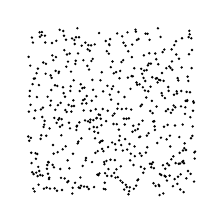
\begin{tikzpicture} 
			\begin{axis}[hide axis,enlargelimits=false,width=3.7cm,height=3.7cm] 
				\addplot[only marks,mark size=0.2pt,mark color={black},samples=500] {rnd^1.0}; 
			\end{axis} 
		\end{tikzpicture}
		\caption{2D CUBE}
		\label{fig:DScube}
	\end{subfigure}%
	\begin{subfigure}{0.50\columnwidth}
		\centering
		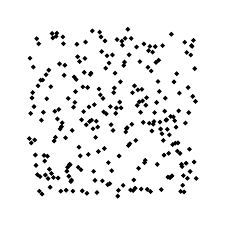
\begin{tikzpicture} 
			\begin{axis}[hide axis,enlargelimits=false,width=3.7cm,height=3.7cm] 
%			\begin{axis}[hide axis,enlargelimits=false,width=4cm,height=4cm] 
				\addplot[only marks,mark size=0.6pt,mark color={black},samples=250] {rnd^1.0}; 
			\end{axis} 
		\end{tikzpicture}
		\caption{2D CLUSTER}
		\label{fig:DScluster}
	\end{subfigure}
	\begin{subfigure}{\columnwidth}
		\centering
		%\includegraphics[width=0.58\textwidth,scale=4]{img/OSM-Alps.png}
		\includegraphics[scale=0.4]{OSM-Alps.png}
		%\epsfig{file=img/OSM-Alps.PNG, scale=0.58}
		\caption{OSM Alps}
		\label{fig:DSosmAlps}
	\end{subfigure}
	\caption{The CUBE, CLUSTER and OSM Alps datasets}
	\label{fig:datasets}
\end{figure}


%\subsection{Rectangle Data}
%The rectangle datasets are constructed in a similar way as the point datasets. 
%For the OSM Alps dataset, we created rectangles as bounding boxes for all line segments in the dataset.
%For the synthetic datasets, each data point becomes a rectangle with randomly generated edge length. Edge lengths vary between 0.0 and $10^{-5}$.
%For CUBE datasets, this results in little to no overlap. CLUSTER data is much denser and therefore likely to overlap. We decided to keep the edge length constant with increasing dimensionality, this means that the probability of overlapping decreases with increasing dimensionality $d$.
%All rectangles are axis-aligned rectangles defined by a 'lower left' and an 'upper right' corner point.


%\todo{Give details to shape and overlap of rectangles}
%
%We also generated an overlap dataset. The idea is to keep the number of pairwise overlaps $o$ as a relative fraction $r$ of the number of elements $N$ with $r=o/N$. For example, assuming a constant $r=0.5$, a dataset with $N=10^6$ rectangles will have about $o=500,000$ pairwise overlaps.
%
%To achieve constant $r$ for datasets with varying size and dimensionality, we vary the average side length $l_{avg} = 1/2*l_{max}$ of the rectangles as follows.
%
%\begin{equation}
		%r = 0.373 k N (l_{avg})^k 2^k \\
		%\Rightarrow \\
		%%\frac{r}{0.373 k N 2^k} = l_{avg}^k \\
		%%\Rightarrow \\
		%(\frac{r}{0.373 k N 2^k})^{1/k} = l_{avg} \\
%\end{equation}
%
%The equation has been developed empirically based on 120 experiments with $100 \leq N \leq 10^6$, $1 \leq k \leq 10$ and $10^{-8} \leq l_{max} \leq 0.8$ for a rectangle cloud between $[0..1]$ in all dimensions. This results ranged between $10^{-6} \leq r \leq 10^3$ ($0 \leq o \leq 2*10^8$). For all our experiments we chose $r=0.5$.

%\subsection{Conventions}
%
%For all diagrams, OSM Alps is abbreviated to OSM, CUBE to CU and CLUSTER to CL. The postfix `-P' indicates point data and `-R' indicates rectangle data. The size of the dataset is denoted by $N$ and the dimensionality by $d$. For all data, we use 64bit floating point values and we ensured that all data points have unique coordinates.



%\section{Outlook}
%\label{sec:outlook}
%
%\subsection{Optimisations}
%
%Numerous optimisations were \emph{not} done, for example:
%
%\begin{itemize}
	%\item Rebalancing for KD-Trees. However a preliminary test indicated that the effect on performance would have been negligible.
	%\item Variation of page sizes of R*Trees and X-Trees. These are known to have strong impact on performance. However we choose very small page sizes as these seemed to result in best performance across all scenarios. Note that these page sizes would have been unrealistically small for a persistent index, resulting in a page size of less than 256 byte (for smaller dimensions).
	%\item The PH-tree performs generally better when used with a data preprocessor~\cite{phtreeRevisitedM}. This usually increases performance by 10\%-30\%, in rare cases by several orders of magnitude, see the 15D CLUSTER 0.5 dataset in~\cite{ZZN2014phtree}.
%\end{itemize}
%
%\begin{itemize}
	%\item Bitstreaming: This is mostly a memory optimisations. Earlier tests with 64bit alignment showed pretty much the same performance (reduced memory (v11) access is outweighted by reduced computation (v10)).
	%\item Object pooling: This certainly makes a difference for the PH-Tree. However, since the PH-Tree has to create key instance for every extraction (queries, etc) and for every element that is inserted (array resizing), the PH-Tree would be unfairly bad. Memory pooling is likely to have much less impact for other index structures.
%\end{itemize}



%\subsection{More Tests}
%
%\begin{itemize}
	%\item Vary overlap of rectangles
	%\item Vary query shapes
%\end{itemize}


%\bibliographystyle{plain}
%\bibliography{sigproc}  % sigproc.bib is the name of the Bibliography in this case


\section{Results}
Results are shown on in the following order:

\begin{itemize}
	\item Insertion: Figures~\ref{fig:loadPerEntry} --~\ref{fig:loadPerEntryDimCL-R}
	\item Memory usage: Figures~\ref{fig:memoryPerEntry} --~\ref{fig:memoryPerEntryDimCL-R}
	\item Window queries: Figures~\ref{fig:wQueryPerEntryP} --~\ref{fig:wqPerEntryDimCL-R}
	\item Exact match queries (point queries): Figures~\ref{fig:pQueryPerEntryP} --~\ref{fig:pQueryDimCL-R}
	\item $k$NN queries: Figures~\ref{fig:1NNQueryPerEntryP} --~\ref{fig:10NNQueryPerEntryDimCL-R}
	\item Update: Figures~\ref{fig:updPerEntryP} --~\ref{fig:updPerEntryDimCL-R}
	\item Remove: Figures~\ref{fig:remPerEntryP} --~\ref{fig:remPerEntryDimCL-R}
\end{itemize}

%\listoffigures
%\newpage

%\subsection{Load}

\begin{figure*}[thb]
	\pgfplotsset{
		every tick label/.append style={font=\scriptsize},
		every axis/.append style={xmode=log, ymode=log, ymin={1e4}, ymax={1e7}, 
				height=7cm, width=6.4cm, grid=major, xlabel={dataset size $N$}, font=\scriptsize, }
	}
%\begin{subfigure}[t]{0.24\textwidth}
	%\begin{tikzpicture} 
	%\pgfplotsset{every axis legend/.append style={ at={(0.05,0.95)}, anchor=south west}}
		%\begin{axis}[ 
			%ylabel={insertions per second},
		%legend columns=3,
		%legend style={draw=none},
		%] 
	%\addplot+[PH] table [selectcoords={0}{7},x=N,y expr=1e9/\thisrow{load/n}, col sep=tab] {sizeP/PHC-P-TIGER(1.0,0.0,null).txt};
	%\addlegendentry{PH} 
	%\addplot+[RSS] table [selectcoords={0}{7},x=N,y expr=1e9/\thisrow{load/n}, col sep=tab] {sizeP/RSS-P-TIGER(1.0,0.0,null).txt};
	%\addlegendentry{RSS} 
	%\addplot+[RSZ] table [selectcoords={0}{7},x=N,y expr=1e9/\thisrow{load/n}, col sep=tab] {sizeP/RSZ-P-TIGER(1.0,0.0,null).txt};
	%\addlegendentry{RSZ} 
	%\addplot+[PHM] table [selectcoords={0}{7},x=N,y expr=1e9/\thisrow{load/n}, col sep=tab] {sizeP/PHC_IPP-P-TIGER(1.0,0.0,null).txt};
	%\addlegendentry{PHM} 
	%\addplot+[STRZ] table [selectcoords={0}{7},x=N,y expr=1e9/\thisrow{load/n}, col sep=tab] {sizeP/STRZ-P-TIGER(1.0,0.0,null).txt};
	%\addlegendentry{STR} 
	%\addplot+[XTS] table [selectcoords={0}{7},x=N,y expr=1e9/\thisrow{load/n}, col sep=tab] {sizeP/XTS-P-TIGER(1.0,0.0,null).txt};
	%\addlegendentry{XTS} 
%%	\addplot+[XTR] table [selectcoords={0}{7},x=N,y expr=1e9/\thisrow{load/n}, col sep=tab] {sizeP/XTR-P-OSM(1.0,0.0,null).txt};
%%	\addlegendentry{XTR} 
	%\addplot+[CBF] table [selectcoords={0}{7},x=N,y expr=1e9/\thisrow{load/n}, col sep=tab] {sizeP/CBF-P-TIGER(1.0,0.0,null).txt};
	%\addlegendentry{CBF} 
	%\addplot+[CBZ] table [selectcoords={0}{7},x=N,y expr=1e9/\thisrow{load/n}, col sep=tab] {sizeP/CBZ-P-TIGER(1.0,0.0,null).txt};
	%\addlegendentry{CBZ} 
	%\addplot+[KDL] table [selectcoords={0}{7},x=N,y expr=1e9/\thisrow{load/n}, col sep=tab] {sizeP/KD_LEVY-P-TIGER(1.0,0.0,null).txt};
	%\addlegendentry{KDL} 
	%\addplot+[KDS] table [selectcoords={0}{7},x=N,y expr=1e9/\thisrow{load/n}, col sep=tab] {sizeP/KD_SAVA-P-TIGER(1.0,0.0,null).txt};
	%\addlegendentry{KDS} 
	%\addplot+[QTZ] table [selectcoords={0}{7},x=N,y expr=1e9/\thisrow{load/n}, col sep=tab] {sizeP/QTZ-P-TIGER(1.0,0.0,null).txt};
	%\addlegendentry{QTZ} 
	%\legend{} %disable legend
		%\end{axis} 
	%\end{tikzpicture}
	%\centering
	%\caption{TIGER-P}
	%\label{fig:loadPerEntryTIG-P}
%%\end{figure}
%\end{subfigure}
\begin{subfigure}[t]{0.33\textwidth}
	\begin{tikzpicture} 
	\pgfplotsset{every axis legend/.append style={ at={(0.02,0.02)}, anchor=south west}}
		\begin{axis}[ 
			ylabel={insertions per second},
			legend columns=3,
			legend style={draw=none},
		] 
	\addplot+[PH] table [selectcoords={0}{7},x=N,y expr=1e9/\thisrow{load/n}, col sep=tab] {sizeP/PHC-P-OSM(1.0,0.0,null).txt};
	\addlegendentry{PH} 
	\addplot+[RSS] table [selectcoords={0}{7},x=N,y expr=1e9/\thisrow{load/n}, col sep=tab] {sizeP/RSS-P-OSM(1.0,0.0,null).txt};
	\addlegendentry{RSS} 
	\addplot+[RSZ] table [selectcoords={0}{7},x=N,y expr=1e9/\thisrow{load/n}, col sep=tab] {sizeP/RSZ-P-OSM(1.0,0.0,null).txt};
	\addlegendentry{RSZ} 
	\addplot+[PHM] table [selectcoords={0}{7},x=N,y expr=1e9/\thisrow{load/n}, col sep=tab] {sizeP/PHC_IPP-P-OSM(1.0,0.0,null).txt};
	\addlegendentry{PHM} 
	\addplot+[STRZ] table [selectcoords={0}{7},x=N,y expr=1e9/\thisrow{load/n}, col sep=tab] {sizeP/STRZ-P-OSM(1.0,0.0,null).txt};
	\addlegendentry{STR} 
	\addplot+[XTS] table [selectcoords={0}{7},x=N,y expr=1e9/\thisrow{load/n}, col sep=tab] {sizeP/XTS-P-OSM(1.0,0.0,null).txt};
	\addlegendentry{XTS} 
%	\addplot+[XTR] table [selectcoords={0}{7},x=N,y expr=1e9/\thisrow{load/n}, col sep=tab] {sizeP/XTR-P-OSM(1.0,0.0,null).txt};
%	\addlegendentry{XTR} 
	\addplot+[CBF] table [selectcoords={0}{7},x=N,y expr=1e9/\thisrow{load/n}, col sep=tab] {sizeP/CBF-P-OSM(1.0,0.0,null).txt};
	\addlegendentry{CBF} 
	\addplot+[CBZ] table [selectcoords={0}{7},x=N,y expr=1e9/\thisrow{load/n}, col sep=tab] {sizeP/CBZ-P-OSM(1.0,0.0,null).txt};
	\addlegendentry{CBZ} 
	\addplot+[KDL] table [selectcoords={0}{7},x=N,y expr=1e9/\thisrow{load/n}, col sep=tab] {sizeP/KD_LEVY-P-OSM(1.0,0.0,null).txt};
	\addlegendentry{KDL} 
	\addplot+[KDS] table [selectcoords={0}{7},x=N,y expr=1e9/\thisrow{load/n}, col sep=tab] {sizeP/KD_SAVA-P-OSM(1.0,0.0,null).txt};
	\addlegendentry{KDS} 
	\addplot+[QTZ] table [selectcoords={0}{7},x=N,y expr=1e9/\thisrow{load/n}, col sep=tab] {sizeP/QTZ-P-OSM(1.0,0.0,null).txt};
	\addlegendentry{QTZ} 
		\end{axis} 
	\end{tikzpicture}
	\centering
	\caption{Alps OSM-P}
	\label{fig:loadPerEntryOSM-P}
%\end{figure}
\end{subfigure}
\begin{subfigure}[t]{0.33\textwidth}
%\begin{figure}[thb]
	\begin{tikzpicture} 
	\pgfplotsset{every axis legend/.append style={ at={(0.05,0.95)}, anchor=north west}}
		\begin{axis}[ 
		legend style={draw=none},
		] 
	\addplot+[PH] table [selectcoords={0}{7},x=N,y expr=1e9/\thisrow{load/n}, col sep=tab] {sizeP/PHC-P-CUBE(1.0,0.0,null).txt};
	\addlegendentry{PH} 
	\addplot+[RSS] table [selectcoords={0}{7},x=N,y expr=1e9/\thisrow{load/n}, col sep=tab] {sizeP/RSS-P-CUBE(1.0,0.0,null).txt};
	\addlegendentry{RSS} 
	\addplot+[RSZ] table [selectcoords={0}{7},x=N,y expr=1e9/\thisrow{load/n}, col sep=tab] {sizeP/RSZ-P-CUBE(1.0,0.0,null).txt};
	\addlegendentry{RSZ} 
	\addplot+[PHM] table [selectcoords={0}{7},x=N,y expr=1e9/\thisrow{load/n}, col sep=tab] {sizeP/PHC_IPP-P-CUBE(1.0,0.0,null).txt};
	\addlegendentry{PHM} 
	\addplot+[STRZ] table [selectcoords={0}{7},x=N,y expr=1e9/\thisrow{load/n}, col sep=tab] {sizeP/STRZ-P-CUBE(1.0,0.0,null).txt};
	\addlegendentry{STR} 
	\addplot+[XTS] table [selectcoords={0}{7},x=N,y expr=1e9/\thisrow{load/n}, col sep=tab] {sizeP/XTS-P-CUBE(1.0,0.0,null).txt};
	\addlegendentry{XTS} 
	\addplot+[CBF] table [selectcoords={0}{7},x=N,y expr=1e9/\thisrow{load/n}, col sep=tab] {sizeP/CBF-P-CUBE(1.0,0.0,null).txt};
	\addlegendentry{CBF} 
	\addplot+[CBZ] table [selectcoords={0}{7},x=N,y expr=1e9/\thisrow{load/n}, col sep=tab] {sizeP/CBZ-P-CUBE(1.0,0.0,null).txt};
	\addlegendentry{CBZ} 
	\addplot+[KDL] table [selectcoords={0}{7},x=N,y expr=1e9/\thisrow{load/n}, col sep=tab] {sizeP/KD_LEVY-P-CUBE(1.0,0.0,null).txt};
	\addlegendentry{KDL} 
	\addplot+[KDS] table [selectcoords={0}{7},x=N,y expr=1e9/\thisrow{load/n}, col sep=tab] {sizeP/KD_SAVA-P-CUBE(1.0,0.0,null).txt};
	\addlegendentry{KDS} 
	\addplot+[QTZ] table [selectcoords={0}{7},x=N,y expr=1e9/\thisrow{load/n}, col sep=tab] {sizeP/QTZ-P-CUBE(1.0,0.0,null).txt};
	\addlegendentry{QTZ} 
	\legend{} %disable legend
		\end{axis} 
	\end{tikzpicture}
	\centering
	\caption{CUBE-P}
	\label{fig:loadPerEntryCU-P}
%\end{figure}
\end{subfigure}
\begin{subfigure}[t]{0.33\textwidth}
%\begin{figure}[thb]
	\begin{tikzpicture} 
	\pgfplotsset{every axis legend/.append style={ at={(0.05,0.95)}, anchor=north west}}
		\begin{axis}[ 
			legend style={draw=none},
		] 
	\addplot+[PH] table [selectcoords={0}{7},x=N,y expr=1e9/\thisrow{load/n}, col sep=tab] {sizeP/PHC-P-CLUSTER(5.0,0.0,null).txt};
	\addlegendentry{PH} 
	\addplot+[RSS] table [selectcoords={0}{7},x=N,y expr=1e9/\thisrow{load/n}, col sep=tab] {sizeP/RSS-P-CLUSTER(5.0,0.0,null).txt};
	\addlegendentry{RSS} 
	\addplot+[RSZ] table [selectcoords={0}{7},x=N,y expr=1e9/\thisrow{load/n}, col sep=tab] {sizeP/RSZ-P-CLUSTER(5.0,0.0,null).txt};
	\addlegendentry{RSZ} 
	\addplot+[PHM] table [selectcoords={0}{7},x=N,y expr=1e9/\thisrow{load/n}, col sep=tab] {sizeP/PHC_IPP-P-CLUSTER(5.0,0.0,null).txt};
	\addlegendentry{PHM} 
	\addplot+[STRZ] table [selectcoords={0}{7},x=N,y expr=1e9/\thisrow{load/n}, col sep=tab] {sizeP/STRZ-P-CLUSTER(5.0,0.0,null).txt};
	\addlegendentry{STR} 
	\addplot+[XTS] table [selectcoords={0}{7},x=N,y expr=1e9/\thisrow{load/n}, col sep=tab] {sizeP/XTS-P-CLUSTER(5.0,0.0,null).txt};
	\addlegendentry{XTS} 
	\addplot+[CBF] table [selectcoords={0}{7},x=N,y expr=1e9/\thisrow{load/n}, col sep=tab] {sizeP/CBF-P-CLUSTER(5.0,0.0,null).txt};
	\addlegendentry{CBF} 
	\addplot+[CBZ] table [selectcoords={0}{7},x=N,y expr=1e9/\thisrow{load/n}, col sep=tab] {sizeP/CBZ-P-CLUSTER(5.0,0.0,null).txt};
	\addlegendentry{CBZ} 
	\addplot+[KDL] table [selectcoords={0}{7},x=N,y expr=1e9/\thisrow{load/n}, col sep=tab] {sizeP/KD_LEVY-P-CLUSTER(5.0,0.0,null).txt};
	\addlegendentry{KDL} 
	\addplot+[KDS] table [selectcoords={0}{7},x=N,y expr=1e9/\thisrow{load/n}, col sep=tab] {sizeP/KD_SAVA-P-CLUSTER(5.0,0.0,null).txt};
	\addlegendentry{KDS} 
	\addplot+[QTZ] table [selectcoords={0}{7},x=N,y expr=1e9/\thisrow{load/n}, col sep=tab] {sizeP/QTZ-P-CLUSTER(5.0,0.0,null).txt};
	\addlegendentry{QTZ} 
	\legend{} %disable legend
		\end{axis} 
	\end{tikzpicture}
	\centering
	\caption{CLUSTER-P}
	\label{fig:loadPerEntryCL-P}
%\end{figure}
\end{subfigure}
	\caption{Point insertion rates for the OSM ($d=2$), CUBE ($d=3$) and CLUSTER ($d=3$) datasets}
	\label{fig:loadPerEntry}
\end{figure*}

\begin{figure*}[thb]
	\pgfplotsset{
		every tick label/.append style={font=\scriptsize},
		every axis/.append style={xmode=log, ymode=log, ymin={1e4}, ymax={1e7}, 
				height=7cm, width=6.4cm, grid=major, xlabel={dataset size $N$}, font=\scriptsize, }
	}
\begin{subfigure}[t]{0.33\textwidth}
	\begin{tikzpicture} 
	\pgfplotsset{every axis legend/.append style={ at={(0.05,0.05)}, anchor=south west}}
		\begin{axis}[ 
			ylabel={insertions per second},
			legend columns=3,
			legend style={draw=none},
		] 
	\addplot+[PH] table [selectcoords={0}{6},x=N,y expr=1e9/\thisrow{load/n}, col sep=tab] {sizeR/PHC-R-OSM(1.0,0.0,null).txt};
	\addlegendentry{PH} 
	\addplot+[RSS] table [selectcoords={0}{6},x=N,y expr=1e9/\thisrow{load/n}, col sep=tab] {sizeR/RSS-R-OSM(1.0,0.0,null).txt};
	\addlegendentry{RSS} 
	\addplot+[RSZ] table [selectcoords={0}{6},x=N,y expr=1e9/\thisrow{load/n}, col sep=tab] {sizeR/RSZ-R-OSM(1.0,0.0,null).txt};
	\addlegendentry{RSZ} 
	\addplot+[PHM] table [selectcoords={0}{6},x=N,y expr=1e9/\thisrow{load/n}, col sep=tab] {sizeR/PHC_IPP-R-OSM(1.0,0.0,null).txt};
	\addlegendentry{PHM} 
	\addplot+[STRZ] table [selectcoords={0}{6},x=N,y expr=1e9/\thisrow{load/n}, col sep=tab] {sizeR/STRZ-R-OSM(1.0,0.0,null).txt};
	\addlegendentry{STR} 
%	\addplot+[XTS] table [selectcoords={0}{6},x=N,y expr=1e9/\thisrow{load/n}, col sep=tab] {sizeR/XTS-R-OSM(1.0,0.0,null).txt};
%	\addlegendentry{XTS} 
	\addplot+[QTZ] table [selectcoords={0}{6},x=N,y expr=1e9/\thisrow{load/n}, col sep=tab] {sizeR/QTZ-R-OSM(1.0,0.0,null).txt};
	\addlegendentry{QTZ} 
		\end{axis} 
	\end{tikzpicture}
	\centering
	\caption{OSM-R}
	\label{fig:loadPerEntryOSM-R}
%\end{figure}
\end{subfigure}
\begin{subfigure}[t]{0.33\textwidth}
%\begin{figure}[thb]
	\begin{tikzpicture} 
	\pgfplotsset{every axis legend/.append style={ at={(0.05,0.95)}, anchor=north west}}
		\begin{axis}[ 
		legend style={draw=none},
		] 
	\addplot+[PH] table [selectcoords={0}{6},x=N,y expr=1e9/\thisrow{load/n}, col sep=tab] {sizeR/PHC-R-CUBE(1.0,0.0,null).txt};
	\addlegendentry{PH} 
	\addplot+[RSS] table [selectcoords={0}{6},x=N,y expr=1e9/\thisrow{load/n}, col sep=tab] {sizeR/RSS-R-CUBE(1.0,0.0,null).txt};
	\addlegendentry{RSS} 
	\addplot+[RSZ] table [selectcoords={0}{6},x=N,y expr=1e9/\thisrow{load/n}, col sep=tab] {sizeR/RSZ-R-CUBE(1.0,0.0,null).txt};
	\addlegendentry{RSZ} 
	\addplot+[PHM] table [selectcoords={0}{6},x=N,y expr=1e9/\thisrow{load/n}, col sep=tab] {sizeR/PHC_IPP-R-CUBE(1.0,0.0,null).txt};
	\addlegendentry{PHM} 
	\addplot+[STRZ] table [selectcoords={0}{6},x=N,y expr=1e9/\thisrow{load/n}, col sep=tab] {sizeR/STRZ-R-CUBE(1.0,0.0,null).txt};
	\addlegendentry{STR} 
%	\addplot+[XTS] table [selectcoords={0}{6},x=N,y expr=1e9/\thisrow{load/n}, col sep=tab] {sizeR/XTS-R-CUBE(1.0,0.0,null).txt};
%	\addlegendentry{XTS} 
	\addplot+[QTZ] table [selectcoords={0}{6},x=N,y expr=1e9/\thisrow{load/n}, col sep=tab] {sizeR/QTZ-R-CUBE(1.0,0.0,null).txt};
	\addlegendentry{QTZ} 
	\legend{} %disable legend
		\end{axis} 
	\end{tikzpicture}
	\centering
	\caption{CUBE-R}
	\label{fig:loadPerEntryCU-R}
%\end{figure}
\end{subfigure}
\begin{subfigure}[t]{0.33\textwidth}
%\begin{figure}[thb]
	\begin{tikzpicture} 
	\pgfplotsset{every axis legend/.append style={ at={(0.05,0.95)}, anchor=north west}}
		\begin{axis}[ 
		legend style={draw=none},
		] 
	\addplot+[PH] table [selectcoords={0}{6},x=N,y expr=1e9/\thisrow{load/n}, col sep=tab] {sizeR/PHC-R-CLUSTER(5.0,0.0,null).txt};
	\addlegendentry{PH} 
	\addplot+[RSS] table [selectcoords={0}{6},x=N,y expr=1e9/\thisrow{load/n}, col sep=tab] {sizeR/RSS-R-CLUSTER(5.0,0.0,null).txt};
	\addlegendentry{RSS} 
	\addplot+[RSZ] table [selectcoords={0}{6},x=N,y expr=1e9/\thisrow{load/n}, col sep=tab] {sizeR/RSZ-R-CLUSTER(5.0,0.0,null).txt};
	\addlegendentry{RSZ} 
	\addplot+[PHM] table [selectcoords={0}{6},x=N,y expr=1e9/\thisrow{load/n}, col sep=tab] {sizeR/PHC_IPP-R-CLUSTER(5.0,0.0,null).txt};
	\addlegendentry{PHM} 
	\addplot+[STRZ] table [selectcoords={0}{6},x=N,y expr=1e9/\thisrow{load/n}, col sep=tab] {sizeR/STRZ-R-CLUSTER(5.0,0.0,null).txt};
	\addlegendentry{STR} 
%	\addplot+[XTS] table [selectcoords={0}{6},x=N,y expr=1e9/\thisrow{load/n}, col sep=tab] {sizeR/XTS-R-CLUSTER(5.0,0.0,null).txt};
%	\addlegendentry{XTS} 
	\addplot+[QTZ] table [selectcoords={0}{6},x=N,y expr=1e9/\thisrow{load/n}, col sep=tab] {sizeR/QTZ-R-CLUSTER(5.0,0.0,null).txt};
	\addlegendentry{QTZ} 
	\legend{} %disable legend
		\end{axis} 
	\end{tikzpicture}
	\centering
	\caption{CLUSTER-R}
	\label{fig:loadPerEntryCL-R}
%\end{figure}
\end{subfigure}
	\caption{Rectangle insertion rates for the OSM ($d=2$), CUBE ($d=3$) and CLUSTER ($d=3$) datasets}
	\label{fig:loadPerEntry-R}
\end{figure*}




%%%%%%%%%%%%%%%
% LOAD CU DIM P
%%%%%%%%%%%%%%%
\begin{figure}[thb]
\begin{tikzpicture}
	\pgfplotsset{every axis legend/.append style={ at={(0.98,0.98)}, anchor=north east}}
\begin{axis}[ 
		%height=9cm, width=9cm, 
		grid=major, 
		xlabel=dimensions,ylabel={insertions per second},
		legend columns=4,
		legend style={draw=none},
		%title={k=2, 64bit, TIGER/Line},
		ymode=log, ymin={1e3}, ymax={5e7},
		%width=6.4cm,ymin={0.08},
		font=\scriptsize,
		%log ticks with fixed point
		] 
	\addplot[CBF] table [selectcoords={0}{9},x=dim,y expr=1e9/\thisrow{load/n}, col sep=tab] {dimsP/CBF-P-CUBE(1.0,0.0,null).txt};
	\addlegendentry{CBF} 
	\addplot[CBZ] table [selectcoords={0}{9},x=dim,y expr=1e9/\thisrow{load/n}, col sep=tab] {dimsP/CBZ-P-CUBE(1.0,0.0,null).txt};
	\addlegendentry{CBZ} 
	\addplot[KDL] table [selectcoords={0}{13},x=dim,y expr=1e9/\thisrow{load/n}, col sep=tab] {dimsP/KD_LEVY-P-CUBE(1.0,0.0,null).txt};
	\addlegendentry{KDL} 
	\addplot[KDS] table [selectcoords={0}{13},x=dim,y expr=1e9/\thisrow{load/n}, col sep=tab] {dimsP/KD_SAVA-P-CUBE(1.0,0.0,null).txt};
	\addlegendentry{KDS} 
	\addplot[PH] table [selectcoords={0}{13},x=dim,y expr=1e9/\thisrow{load/n}, col sep=tab] {dimsP/PHC-P-CUBE(1.0,0.0,null).txt};
	\addlegendentry{PH} 
	\addplot[PHM] table [selectcoords={0}{13},x=dim,y expr=1e9/\thisrow{load/n}, col sep=tab] {dimsP/PHC_IPP-P-CUBE(1.0,0.0,null).txt};
	\addlegendentry{PHM} 
	\addplot[QTZ] table [selectcoords={0}{8},x=dim,y expr=1e9/\thisrow{load/n}, col sep=tab] {dimsP/QTZ-P-CUBE(1.0,0.0,null).txt};
	\addlegendentry{QTZ} 
	\addplot[RSS] table [selectcoords={0}{13},x=dim,y expr=1e9/\thisrow{load/n}, col sep=tab] {dimsP/RSS-P-CUBE(1.0,0.0,null).txt};
	\addlegendentry{RSS} 
	\addplot[RSZ] table [selectcoords={0}{13},x=dim,y expr=1e9/\thisrow{load/n}, col sep=tab] {dimsP/RSZ-P-CUBE(1.0,0.0,null).txt};
	\addlegendentry{RSZ} 
	\addplot[STRZ] table [selectcoords={0}{13},x=dim,y expr=1e9/\thisrow{load/n}, col sep=tab] {dimsP/STRZ-P-CUBE(1.0,0.0,null).txt};
	\addlegendentry{STRZ} 
	\addplot[XTS] table [selectcoords={0}{13},x=dim,y expr=1e9/\thisrow{load/n}, col sep=tab] {dimsP/XTS-P-CUBE(1.0,0.0,null).txt};
	\addlegendentry{XTS} 
\end{axis}
\end{tikzpicture}
	\centering
	\caption{DIM: Insertion rates for CU-P with $N=10^6$}
	\label{fig:loadPerEntryDimCU-P}
\end{figure}

%%%%%%%%%%%%%%%
% LOAD CU DIM R
%%%%%%%%%%%%%%%
\begin{figure}[thb]
\begin{tikzpicture}
	\pgfplotsset{every axis legend/.append style={ at={(0.02,0.02)}, anchor=south west}}
\begin{axis}[ 
		%height=9cm, width=9cm, 
		grid=major, 
		xlabel=dimensions,ylabel={insertions per second},
		legend columns=2,
		legend style={draw=none},
		%title={k=2, 64bit, TIGER/Line},
		ymode=log, ymin={1e3}, ymax={1e7},
		%width=6.4cm,ymin={0.08},
		font=\scriptsize,
		%log ticks with fixed point
		] 
	\addplot+[PH] table [selectcoords={0}{11},x=dim,y expr=1e9/\thisrow{load/n}, col sep=tab] {dimsR/PHC-R-CUBE(1.0,0.0,null).txt};
	\addlegendentry{PH} 
	\addplot+[PHM] table [selectcoords={0}{11},x=dim,y expr=1e9/\thisrow{load/n}, col sep=tab] {dimsR/PHC_IPP-R-CUBE(1.0,0.0,null).txt};
	\addlegendentry{PHM} 
	\addplot+[RSS] table [selectcoords={0}{11},x=dim,y expr=1e9/\thisrow{load/n}, col sep=tab] {dimsR/RSS-R-CUBE(1.0,0.0,null).txt};
	\addlegendentry{RSS} 
	\addplot+[RSZ] table [selectcoords={0}{11},x=dim,y expr=1e9/\thisrow{load/n}, col sep=tab] {dimsR/RSZ-R-CUBE(1.0,0.0,null).txt};
	\addlegendentry{RSZ} 
	\addplot+[STRZ] table [selectcoords={0}{11},x=dim,y expr=1e9/\thisrow{load/n}, col sep=tab] {dimsR/STRZ-R-CUBE(1.0,0.0,null).txt};
	\addlegendentry{STRZ} 
	\addplot+[QTZ] table [selectcoords={0}{11},x=dim,y expr=1e9/\thisrow{load/n}, col sep=tab] {dimsR/QTZ-R-CUBE(1.0,0.0,null).txt};
	\addlegendentry{QTZ} 
\end{axis}
\end{tikzpicture}
	\centering
	\caption{DIM: Insertion rates for CU-R with $N=10^6$}
	\label{fig:loadPerEntryDimCU-R}
\end{figure}

%%%%%%%%%%%%%%%
% LOAD CL DIM P
%%%%%%%%%%%%%%%
\begin{figure}[thb]
\begin{tikzpicture}
	\pgfplotsset{every axis legend/.append style={ at={(0.98,0.98)}, anchor=north east}}
\begin{axis}[ 
		%height=9cm, width=9cm, 
		grid=major, 
		xlabel=dimensions,ylabel={insertions per second},
		legend columns=4,
		legend style={draw=none},
		%title={k=2, 64bit, TIGER/Line},
		ymode=log, ymin={1e3}, ymax={7e7},
		%width=6.4cm,ymin={0.08},
		font=\scriptsize,
		%log ticks with fixed point
		] 
	\addplot[CBF] table [selectcoords={0}{9},x=dim,y expr=1e9/\thisrow{load/n}, col sep=tab] {dimsP/CBF-P-CLUSTER(5.0,0.0,null).txt};
	\addlegendentry{CBF} 
	\addplot[CBZ] table [selectcoords={0}{9},x=dim,y expr=1e9/\thisrow{load/n}, col sep=tab] {dimsP/CBZ-P-CLUSTER(5.0,0.0,null).txt};
	\addlegendentry{CBZ} 
	\addplot[KDL] table [selectcoords={0}{13},x=dim,y expr=1e9/\thisrow{load/n}, col sep=tab] {dimsP/KD_LEVY-P-CLUSTER(5.0,0.0,null).txt};
	\addlegendentry{KDL} 
	\addplot[KDS] table [selectcoords={0}{13},x=dim,y expr=1e9/\thisrow{load/n}, col sep=tab] {dimsP/KD_SAVA-P-CLUSTER(5.0,0.0,null).txt};
	\addlegendentry{KDS} 
	\addplot[PH] table [selectcoords={0}{13},x=dim,y expr=1e9/\thisrow{load/n}, col sep=tab] {dimsP/PHC-P-CLUSTER(5.0,0.0,null).txt};
	\addlegendentry{PH} 
	\addplot[PHM] table [selectcoords={0}{15},x=dim,y expr=1e9/\thisrow{load/n}, col sep=tab] {dimsP/PHC_IPP-P-CLUSTER(5.0,0.0,null).txt};
	\addlegendentry{PHM} 
	\addplot[QTZ] table [selectcoords={0}{8},x=dim,y expr=1e9/\thisrow{load/n}, col sep=tab] {dimsP/QTZ-P-CLUSTER(5.0,0.0,null).txt};
	\addlegendentry{QTZ} 
	\addplot[RSS] table [selectcoords={0}{13},x=dim,y expr=1e9/\thisrow{load/n}, col sep=tab] {dimsP/RSS-P-CLUSTER(5.0,0.0,null).txt};
	\addlegendentry{RSS} 
	\addplot[RSZ] table [selectcoords={0}{13},x=dim,y expr=1e9/\thisrow{load/n}, col sep=tab] {dimsP/RSZ-P-CLUSTER(5.0,0.0,null).txt};
	\addlegendentry{RSZ} 
	\addplot[STRZ] table [selectcoords={0}{13},x=dim,y expr=1e9/\thisrow{load/n}, col sep=tab] {dimsP/STRZ-P-CLUSTER(5.0,0.0,null).txt};
	\addlegendentry{STRZ} 
	\addplot[XTS] table [selectcoords={0}{13},x=dim,y expr=1e9/\thisrow{load/n}, col sep=tab] {dimsP/XTS-P-CLUSTER(5.0,0.0,null).txt};
	\addlegendentry{XTS} 
\end{axis}
\end{tikzpicture}
	\centering
	\caption{DIM: Insertion rates for CL-P with $N=10^6$}
	\label{fig:loadPerEntryDimCL-P}
\end{figure}

%%%%%%%%%%%%%%%
% LOAD CU DIM R
%%%%%%%%%%%%%%%
\begin{figure}[thb]
\begin{tikzpicture}
	\pgfplotsset{every axis legend/.append style={ at={(0.02,0.02)}, anchor=south west}}
\begin{axis}[ 
		%height=9cm, width=9cm, 
		grid=major, 
		xlabel=dimensions,ylabel={insertions per second},
		legend columns=2,
		legend style={draw=none},
		%title={k=2, 64bit, TIGER/Line},
		ymode=log, ymin={1e3},
		%width=6.4cm,ymin={0.08},
		font=\scriptsize,
		%log ticks with fixed point
		] 
	\addplot+[PH] table [selectcoords={0}{11},x=dim,y expr=1e9/\thisrow{load/n}, col sep=tab] {dimsR/PHC-R-CLUSTER(5.0,0.0,null).txt};
	\addlegendentry{PH} 
	\addplot+[PHM] table [selectcoords={0}{11},x=dim,y expr=1e9/\thisrow{load/n}, col sep=tab] {dimsR/PHC_IPP-R-CLUSTER(5.0,0.0,null).txt};
	\addlegendentry{PHM} 
	\addplot+[RSS] table [selectcoords={0}{11},x=dim,y expr=1e9/\thisrow{load/n}, col sep=tab] {dimsR/RSS-R-CLUSTER(5.0,0.0,null).txt};
	\addlegendentry{RSS} 
	\addplot+[RSZ] table [selectcoords={0}{11},x=dim,y expr=1e9/\thisrow{load/n}, col sep=tab] {dimsR/RSZ-R-CLUSTER(5.0,0.0,null).txt};
	\addlegendentry{RSZ} 
	\addplot+[STRZ] table [selectcoords={0}{11},x=dim,y expr=1e9/\thisrow{load/n}, col sep=tab] {dimsR/STRZ-R-CLUSTER(5.0,0.0,null).txt};
	\addlegendentry{STRZ} 
	\addplot+[QTZ] table [selectcoords={0}{11},x=dim,y expr=1e9/\thisrow{load/n}, col sep=tab] {dimsR/QTZ-R-CLUSTER(5.0,0.0,null).txt};
	\addlegendentry{QTZ} 
\end{axis}
\end{tikzpicture}
	\centering
	\caption{DIM: Insertion rates for CL-R with $N=10^6$}
	\label{fig:loadPerEntryDimCL-R}
\end{figure}

\clearpage
\newpage

%\subsection{Memory Usage}
%\label{sec:memory}

%\begin{figure}[thb]
\begin{figure*}[thb]
\begin{subfigure}[t]{0.33\textwidth}
	\begin{tikzpicture} 
	\pgfplotsset{every axis legend/.append style={ at={(0.05,0.98)}, anchor=north west}}
		\begin{axis}[ 
		height=7cm, width=6.4cm, 
		grid=major, 
		xlabel=$10^6$ entries, ylabel={ns per entry},
		%title={k=2, 64bit, TIGER/Line},
		legend columns=3,
		legend style={draw=none},
		font=\scriptsize,
		%ymode=log, 
		ymin={0}, ymax={200},
		xmode=log, 
		] 
	\addplot+[PH] table [selectcoords={0}{7},x expr=\thisrow{N}/1000000,y=memory/n, col sep=tab] {sizeP/PHC-P-OSM(1.0,0.0,null).txt};
	\addlegendentry{PH} 
	\addplot+[RSS] table [selectcoords={0}{7},x expr=\thisrow{N}/1000000,y=memory/n, col sep=tab] {sizeP/RSS-P-OSM(1.0,0.0,null).txt};
	\addlegendentry{RSS} 
	\addplot+[RSZ] table [selectcoords={0}{7},x expr=\thisrow{N}/1000000,y=memory/n, col sep=tab] {sizeP/RSZ-P-OSM(1.0,0.0,null).txt};
	\addlegendentry{RSZ} 
	\addplot+[PHM] table [selectcoords={0}{7},x expr=\thisrow{N}/1000000,y=memory/n, col sep=tab] {sizeP/PHC_IPP-P-OSM(1.0,0.0,null).txt};
	\addlegendentry{PHM} 
	\addplot+[STRZ] table [selectcoords={0}{7},x expr=\thisrow{N}/1000000,y=memory/n, col sep=tab] {sizeP/STRZ-P-OSM(1.0,0.0,null).txt};
	\addlegendentry{STR} 
	\addplot+[XTS] table [selectcoords={0}{7},x expr=\thisrow{N}/1000000,y=memory/n, col sep=tab] {sizeP/XTS-P-OSM(1.0,0.0,null).txt};
	\addlegendentry{XTS} 
%	\addplot+[XTR] table [selectcoords={0}{7},x expr=\thisrow{N}/1000000,y=memory/n, col sep=tab] {sizeP/XTR-P-OSM(1.0,0.0,null).txt};
%	\addlegendentry{XTR} 
	\addplot+[CBF] table [selectcoords={0}{7},x expr=\thisrow{N}/1000000,y=memory/n, col sep=tab] {sizeP/CBF-P-OSM(1.0,0.0,null).txt};
	\addlegendentry{CBF} 
	\addplot+[CBZ] table [selectcoords={0}{7},x expr=\thisrow{N}/1000000,y=memory/n, col sep=tab] {sizeP/CBZ-P-OSM(1.0,0.0,null).txt};
	\addlegendentry{CBZ} 
	\addplot+[KDL] table [selectcoords={0}{7},x expr=\thisrow{N}/1000000,y=memory/n, col sep=tab] {sizeP/KD_LEVY-P-OSM(1.0,0.0,null).txt};
	\addlegendentry{KDL} 
	\addplot+[KDS] table [selectcoords={0}{7},x expr=\thisrow{N}/1000000,y=memory/n, col sep=tab] {sizeP/KD_SAVA-P-OSM(1.0,0.0,null).txt};
	\addlegendentry{KDS} 
	\addplot+[QTZ] table [selectcoords={0}{7},x expr=\thisrow{N}/1000000,y=memory/n, col sep=tab] {sizeP/QTZ-P-OSM(1.0,0.0,null).txt};
	\addlegendentry{QTZ} 
		\end{axis} 
	\end{tikzpicture}
	\centering
	\caption{Alps OSM-P}
	\label{fig:memoryPerEntryOSM-P}
%\end{figure}
\end{subfigure}
\begin{subfigure}[t]{0.33\textwidth}
%\begin{figure}[thb]
	\begin{tikzpicture} 
	\pgfplotsset{every axis legend/.append style={ at={(0.05,0.95)}, anchor=north west}}
		\begin{axis}[ 
		height=7cm, width=6.4cm, 
		grid=major, 
		xlabel=$10^6$ entries, %ylabel={ns per entry},
		%title={k=2, 64bit, TIGER/Line},
		legend style={draw=none},
		font=\scriptsize,
		%ymode=log, 
		ymin={0}, ymax={200},
		xmode=log, 
		] 
	\addplot+[PH] table [selectcoords={0}{7},x expr=\thisrow{N}/1000000,y=memory/n, col sep=tab] {sizeP/PHC-P-CUBE(1.0,0.0,null).txt};
	\addlegendentry{PH} 
	\addplot+[RSS] table [selectcoords={0}{7},x expr=\thisrow{N}/1000000,y=memory/n, col sep=tab] {sizeP/RSS-P-CUBE(1.0,0.0,null).txt};
	\addlegendentry{RSS} 
	\addplot+[RSZ] table [selectcoords={0}{7},x expr=\thisrow{N}/1000000,y=memory/n, col sep=tab] {sizeP/RSZ-P-CUBE(1.0,0.0,null).txt};
	\addlegendentry{RSZ} 
	\addplot+[PHM] table [selectcoords={0}{7},x expr=\thisrow{N}/1000000,y=memory/n, col sep=tab] {sizeP/PHC_IPP-P-CUBE(1.0,0.0,null).txt};
	\addlegendentry{PHM} 
	\addplot+[STRZ] table [selectcoords={0}{7},x expr=\thisrow{N}/1000000,y=memory/n, col sep=tab] {sizeP/STRZ-P-CUBE(1.0,0.0,null).txt};
	\addlegendentry{STR} 
	\addplot+[XTS] table [selectcoords={0}{7},x expr=\thisrow{N}/1000000,y=memory/n, col sep=tab] {sizeP/XTS-P-CUBE(1.0,0.0,null).txt};
	\addlegendentry{XTS} 
	\addplot+[CBF] table [selectcoords={0}{7},x expr=\thisrow{N}/1000000,y=memory/n, col sep=tab] {sizeP/CBF-P-CUBE(1.0,0.0,null).txt};
	\addlegendentry{CBF} 
	\addplot+[CBZ] table [selectcoords={0}{7},x expr=\thisrow{N}/1000000,y=memory/n, col sep=tab] {sizeP/CBZ-P-CUBE(1.0,0.0,null).txt};
	\addlegendentry{CBZ} 
	\addplot+[KDL] table [selectcoords={0}{7},x expr=\thisrow{N}/1000000,y=memory/n, col sep=tab] {sizeP/KD_LEVY-P-CUBE(1.0,0.0,null).txt};
	\addlegendentry{KDL} 
	\addplot+[KDS] table [selectcoords={0}{7},x expr=\thisrow{N}/1000000,y=memory/n, col sep=tab] {sizeP/KD_SAVA-P-CUBE(1.0,0.0,null).txt};
	\addlegendentry{KDS} 
	\addplot+[QTZ] table [selectcoords={0}{7},x expr=\thisrow{N}/1000000,y=memory/n, col sep=tab] {sizeP/QTZ-P-CUBE(1.0,0.0,null).txt};
	\addlegendentry{QTZ} 
	\legend{} %disable legend
		\end{axis} 
	\end{tikzpicture}
	\centering
	\caption{CUBE-P}
	\label{fig:memoryPerEntryCU-P}
%\end{figure}
\end{subfigure}
\begin{subfigure}[t]{0.33\textwidth}
%\begin{figure}[thb]
	\begin{tikzpicture} 
	\pgfplotsset{every axis legend/.append style={ at={(0.05,0.95)}, anchor=north west}}
		\begin{axis}[ 
		height=7cm, width=6.4cm, 
		grid=major, 
		xlabel=$10^6$ entries, %ylabel={ns per entry},
		%title={k=2, 64bit, TIGER/Line},
		legend style={draw=none},
		font=\scriptsize,
		%ymode=log, 
		ymin={0}, ymax={200},
		xmode=log, 
		] 
	\addplot+[PH] table [selectcoords={0}{7},x expr=\thisrow{N}/1000000,y=memory/n, col sep=tab] {sizeP/PHC-P-CLUSTER(5.0,0.0,null).txt};
	\addlegendentry{PH} 
	\addplot+[RSS] table [selectcoords={0}{7},x expr=\thisrow{N}/1000000,y=memory/n, col sep=tab] {sizeP/RSS-P-CLUSTER(5.0,0.0,null).txt};
	\addlegendentry{RSS} 
	\addplot+[RSZ] table [selectcoords={0}{7},x expr=\thisrow{N}/1000000,y=memory/n, col sep=tab] {sizeP/RSZ-P-CLUSTER(5.0,0.0,null).txt};
	\addlegendentry{RSZ} 
	\addplot+[PHM] table [selectcoords={0}{7},x expr=\thisrow{N}/1000000,y=memory/n, col sep=tab] {sizeP/PHC_IPP-P-CLUSTER(5.0,0.0,null).txt};
	\addlegendentry{PHM} 
	\addplot+[STRZ] table [selectcoords={0}{7},x expr=\thisrow{N}/1000000,y=memory/n, col sep=tab] {sizeP/STRZ-P-CLUSTER(5.0,0.0,null).txt};
	\addlegendentry{STR} 
	\addplot+[XTS] table [selectcoords={0}{7},x expr=\thisrow{N}/1000000,y=memory/n, col sep=tab] {sizeP/XTS-P-CLUSTER(5.0,0.0,null).txt};
	\addlegendentry{XTS} 
	\addplot+[CBF] table [selectcoords={0}{7},x expr=\thisrow{N}/1000000,y=memory/n, col sep=tab] {sizeP/CBF-P-CLUSTER(5.0,0.0,null).txt};
	\addlegendentry{CBF} 
	\addplot+[CBZ] table [selectcoords={0}{7},x expr=\thisrow{N}/1000000,y=memory/n, col sep=tab] {sizeP/CBZ-P-CLUSTER(5.0,0.0,null).txt};
	\addlegendentry{CBZ} 
	\addplot+[KDL] table [selectcoords={0}{7},x expr=\thisrow{N}/1000000,y=memory/n, col sep=tab] {sizeP/KD_LEVY-P-CLUSTER(5.0,0.0,null).txt};
	\addlegendentry{KDL} 
	\addplot+[KDS] table [selectcoords={0}{7},x expr=\thisrow{N}/1000000,y=memory/n, col sep=tab] {sizeP/KD_SAVA-P-CLUSTER(5.0,0.0,null).txt};
	\addlegendentry{KDS} 
	\addplot+[QTZ] table [selectcoords={0}{7},x expr=\thisrow{N}/1000000,y=memory/n, col sep=tab] {sizeP/QTZ-P-CLUSTER(5.0,0.0,null).txt};
	\addlegendentry{QTZ} 
	\legend{} %disable legend
		\end{axis} 
	\end{tikzpicture}
	\centering
	\caption{CLUSTER-P}
	\label{fig:memoryPerEntryCL-P}
%\end{figure}
\end{subfigure}
	\caption{Memory usage per point entry for the OSM Alps, CUBE and CLUSTER datasets}
	\label{fig:memoryPerEntry}
\end{figure*}


\begin{figure*}[thb]
\begin{subfigure}[t]{0.33\textwidth}
	\begin{tikzpicture} 
	\pgfplotsset{every axis legend/.append style={ at={(0.05,0.95)}, anchor=north west}}
		\begin{axis}[ 
		height=7cm, width=6.4cm, 
		grid=major, 
		xlabel=$10^6$ entries, ylabel={ns per entry},
		%title={k=2, 64bit, TIGER/Line},
		legend columns=3,
		legend style={draw=none},
		font=\scriptsize,
		%ymode=log, 
		ymin={0}, ymax={200},
		xmode=log, 
		] 
	\addplot+[PH] table [selectcoords={0}{7},x expr=\thisrow{N}/1000000,y=memory/n, col sep=tab] {sizeR/PHC-R-OSM(1.0,0.0,null).txt};
	\addlegendentry{PH} 
	\addplot+[RSS] table [selectcoords={0}{7},x expr=\thisrow{N}/1000000,y=memory/n, col sep=tab] {sizeR/RSS-R-OSM(1.0,0.0,null).txt};
	\addlegendentry{RSS} 
	\addplot+[RSZ] table [selectcoords={0}{7},x expr=\thisrow{N}/1000000,y=memory/n, col sep=tab] {sizeR/RSZ-R-OSM(1.0,0.0,null).txt};
	\addlegendentry{RSZ} 
	\addplot+[PHM] table [selectcoords={0}{7},x expr=\thisrow{N}/1000000,y=memory/n, col sep=tab] {sizeR/PHC_IPP-R-OSM(1.0,0.0,null).txt};
	\addlegendentry{PHM} 
	\addplot+[STRZ] table [selectcoords={0}{7},x expr=\thisrow{N}/1000000,y=memory/n, col sep=tab] {sizeR/STRZ-R-OSM(1.0,0.0,null).txt};
	\addlegendentry{STR} 
%	\addplot+[XTS] table [selectcoords={0}{7},x expr=\thisrow{N}/1000000,y=memory/n, col sep=tab] {sizeR/XTS-R-OSM(1.0,0.0,null).txt};
%	\addlegendentry{XTS} 
	\addplot+[QTZ] table [selectcoords={0}{7},x expr=\thisrow{N}/1000000,y=memory/n, col sep=tab] {sizeR/QTZ-R-OSM(1.0,0.0,null).txt};
	\addlegendentry{QTZ} 
		\end{axis} 
	\end{tikzpicture}
	\centering
	\caption{Alps OSM-R}
	\label{fig:memoryPerEntryOSM-R}
%\end{figure}
\end{subfigure}
\begin{subfigure}[t]{0.33\textwidth}
%\begin{figure}[thb]
	\begin{tikzpicture} 
	\pgfplotsset{every axis legend/.append style={ at={(0.05,0.95)}, anchor=north west}}
		\begin{axis}[ 
		height=7cm, width=6.4cm, 
		grid=major, 
		xlabel=$10^6$ entries, %ylabel={$\mu$s per entry},
		%title={k=2, 64bit, TIGER/Line},
		legend style={draw=none},
		font=\scriptsize,
		%ymode=log, 
		ymin={0}, ymax={200},
		xmode=log, 
		] 
	\addplot+[PH] table [selectcoords={0}{7},x expr=\thisrow{N}/1000000,y=memory/n, col sep=tab] {sizeR/PHC-R-CUBE(1.0,0.0,null).txt};
	\addlegendentry{PH} 
	\addplot+[RSS] table [selectcoords={0}{7},x expr=\thisrow{N}/1000000,y=memory/n, col sep=tab] {sizeR/RSS-R-CUBE(1.0,0.0,null).txt};
	\addlegendentry{RSS} 
	\addplot+[RSZ] table [selectcoords={0}{7},x expr=\thisrow{N}/1000000,y=memory/n, col sep=tab] {sizeR/RSZ-R-CUBE(1.0,0.0,null).txt};
	\addlegendentry{RSZ} 
	\addplot+[PHM] table [selectcoords={0}{7},x expr=\thisrow{N}/1000000,y=memory/n, col sep=tab] {sizeR/PHC_IPP-R-CUBE(1.0,0.0,null).txt};
	\addlegendentry{PHM} 
	\addplot+[STRZ] table [selectcoords={0}{7},x expr=\thisrow{N}/1000000,y=memory/n, col sep=tab] {sizeR/STRZ-R-CUBE(1.0,0.0,null).txt};
	\addlegendentry{STR} 
%	\addplot+[XTS] table [selectcoords={0}{7},x expr=\thisrow{N}/1000000,y=memory/n, col sep=tab] {sizeR/XTS-R-CUBE(1.0,0.0,null).txt};
%	\addlegendentry{XTS} 
	\addplot+[QTZ] table [selectcoords={0}{7},x expr=\thisrow{N}/1000000,y=memory/n, col sep=tab] {sizeR/QTZ-R-CUBE(1.0,0.0,null).txt};
	\addlegendentry{QTZ} 
	\legend{} %disable legend
		\end{axis} 
	\end{tikzpicture}
	\centering
	\caption{CUBE-R}
	\label{fig:memoryPerEntryCU-R}
%\end{figure}
\end{subfigure}
\begin{subfigure}[t]{0.33\textwidth}
%\begin{figure}[thb]
	\begin{tikzpicture} 
	\pgfplotsset{every axis legend/.append style={ at={(0.05,0.95)}, anchor=north west}}
		\begin{axis}[ 
		height=7cm, width=6.4cm, 
		grid=major, 
		xlabel=$10^6$ entries, %ylabel={$\mu$s per entry},
		%title={k=2, 64bit, TIGER/Line},
		legend style={draw=none},
		font=\scriptsize,
		%ymode=log, 
		ymin={0}, ymax={200},
		xmode=log, 
		] 
	\addplot+[PH] table [selectcoords={0}{7},x expr=\thisrow{N}/1000000,y=memory/n, col sep=tab] {sizeR/PHC-R-CLUSTER(5.0,0.0,null).txt};
	\addlegendentry{PH} 
	\addplot+[RSS] table [selectcoords={0}{7},x expr=\thisrow{N}/1000000,y=memory/n, col sep=tab] {sizeR/RSS-R-CLUSTER(5.0,0.0,null).txt};
	\addlegendentry{RSS} 
	\addplot+[RSZ] table [selectcoords={0}{7},x expr=\thisrow{N}/1000000,y=memory/n, col sep=tab] {sizeR/RSZ-R-CLUSTER(5.0,0.0,null).txt};
	\addlegendentry{RSZ} 
	\addplot+[PHM] table [selectcoords={0}{7},x expr=\thisrow{N}/1000000,y=memory/n, col sep=tab] {sizeR/PHC_IPP-R-CLUSTER(5.0,0.0,null).txt};
	\addlegendentry{PHM} 
	\addplot+[STRZ] table [selectcoords={0}{7},x expr=\thisrow{N}/1000000,y=memory/n, col sep=tab] {sizeR/STRZ-R-CLUSTER(5.0,0.0,null).txt};
	\addlegendentry{STR} 
%	\addplot+[XTS] table [selectcoords={0}{7},x expr=\thisrow{N}/1000000,y=memory/n, col sep=tab] {sizeR/XTS-R-CLUSTER(5.0,0.0,null).txt};
%	\addlegendentry{XTS} 
	\addplot+[QTZ] table [selectcoords={0}{7},x expr=\thisrow{N}/1000000,y=memory/n, col sep=tab] {sizeR/QTZ-R-CLUSTER(5.0,0.0,null).txt};
	\addlegendentry{QTZ} 
	\legend{} %disable legend
		\end{axis} 
	\end{tikzpicture}
	\centering
	\caption{CLUSTER-R}
	\label{fig:memoryPerEntryCL-R}
%\end{figure}
\end{subfigure}
	\caption{Memory usage per rectangle entry for the OSM Alps, CUBE and CLUSTER datasets}
	\label{fig:memoryPerEntry-R}
\end{figure*}


\input{DiagramsMemory-Dims}
\clearpage
\newpage

\input{DiagramsWindowQuery-Size}
%%%%%%%%%%%%%%%
% Window queries
%%%%%%%%%%%%%%%
%\subsection{Window Query}



%%%%%%%%%%%
% W QUERY small/big
%%%%%%%%%%%
% BIG TRICK: for X we can use the query result column!!
% -> We could divide this by 1000(?) to get average result size!
%%%%%%%%%%%
%\begin{figure}%[thb]
%\begin{tikzpicture}
	%\pgfplotsset{every axis legend/.append style={ at={(0.95,0.95)}, anchor=north east}}
%\begin{axis}[ 
		%height=7cm, width=6.4cm, 
		%grid=major, 
		%xlabel=Average query result size,ylabel={ns per returned entry},
		%legend columns=2,
		%legend style={draw=none},
		%%title={k=2, 64bit, TIGER/Line},
		%ymode=log,
		%%width=6.4cm,ymin={0.08},
		%%xmax=30000000,xmin=0,
		%%scaled x ticks=base 10:6,
		%font=\scriptsize,
		%%log ticks with fixed point
		%ymode=log, ymin={50}, ymax={10e4},
		%xmode=log, 
		%] 
	%\addplot+[PH] table [selectcoords={0}{5},x expr=\thisrow{q2-n}/1000,y=q2/n, col sep=tab] {sizePWQS/PHC-P-CUBE(1.0,0.0,null).txt};
	%\addlegendentry{PH} 
	%\addplot+[RSS] table [selectcoords={0}{5},x expr=\thisrow{q2-n}/1000,y=q2/n, col sep=tab] {sizePWQS/RSS-P-CUBE(1.0,0.0,null).txt};
	%\addlegendentry{RSS} 
	%\addplot+[RSZ] table [selectcoords={0}{5},x expr=\thisrow{q2-n}/1000,y=q2/n, col sep=tab] {sizePWQS/RSZ-P-CUBE(1.0,0.0,null).txt};
	%\addlegendentry{RSZ} 
	%\addplot+[PHM] table [selectcoords={0}{5},x expr=\thisrow{q2-n}/1000,y=q2/n, col sep=tab] {sizePWQS/PHC_IPP-P-CUBE(1.0,0.0,null).txt};
	%\addlegendentry{PHM} 
%%	\addplot+[CBF] table [selectcoords={0}{5},x expr=\thisrow{q2-n}/1000,y=q2/n, col sep=tab] {sizePWQS/CBF-P-CUBE(1.0,0.0,null).txt};
%%	\addlegendentry{CBF} 
%%	\addplot+[CBZ] table [selectcoords={0}{5},x expr=\thisrow{q2-n}/1000,y=q2/n, col sep=tab] {sizePWQS/CBZ-P-CUBE(1.0,0.0,null).txt};
%%	\addlegendentry{CBZ} 
	%\addplot+[KDL] table [selectcoords={0}{5},x expr=\thisrow{q2-n}/1000,y=q2/n, col sep=tab] {sizePWQS/KD_LEVY-P-CUBE(1.0,0.0,null).txt};
	%\addlegendentry{KDL} 
	%\addplot+[KDS] table [selectcoords={0}{5},x expr=\thisrow{q2-n}/1000,y=q2/n, col sep=tab] {sizePWQS/KD_SAVA-P-CUBE(1.0,0.0,null).txt};
	%\addlegendentry{KDS} 
	%\addplot+[QKDZ] table [selectcoords={0}{5},x expr=\thisrow{q2-n}/1000,y=q2/n, col sep=tab] {sizePWQS/QKDZ-P-CUBE(1.0,0.0,null).txt};
	%\addlegendentry{QZ} 
	%\addplot+[STRZ] table [selectcoords={0}{5},x expr=\thisrow{q2-n}/1000,y=q2/n, col sep=tab] {sizePWQS/STRZ-P-CUBE(1.0,0.0,null).txt};
	%\addlegendentry{STR} 
	%\addplot+[XTS] table [selectcoords={0}{5},x expr=\thisrow{q2-n}/1000,y=q2/n, col sep=tab] {sizePWQS/XTS-P-CUBE(1.0,0.0,null).txt};
	%\addlegendentry{XTS} 
%%  \addplot+[XTR] table [selectcoords={0}{5},x expr=\thisrow{q2-n}/1000,y=q2/n, col sep=tab] {sizePWQS/XTR-P-CUBE(1.0,0.0,null).txt};
%%	\addlegendentry{XTR} 
%\end{axis}
%\end{tikzpicture}
	%\centering
	%\caption{Varying query result size with CU-P}
	%\label{fig:wQueryVarSizeOSM-P}
%\end{figure}

\begin{figure*}%[thb]
	\pgfplotsset{
		every tick label/.append style={font=\scriptsize},
		every axis/.append style={xmode=log, ymode=log, ymin={1e2}, ymax={1e7}, 
				height=7cm, width=6.4cm, grid=major, xlabel={dataset size $N$}, font=\scriptsize, }
	}
\begin{subfigure}[t]{0.33\textwidth}
\begin{tikzpicture}
	\pgfplotsset{every axis legend/.append style={ at={(0.98,0.98)}, anchor=north east, legend columns=2}}
		\begin{axis}[ 
			ylabel={queries per second},
			legend columns=2,
			legend style={draw=none},
		] 
	\addplot+[PH] table [selectcoords={0}{4},x expr=\thisrow{q2-n}/10000,y expr=1e9/(\thisrow{q2/n}*\thisrow{q2-n})*10000, col sep=tab] {sizePWQS/PHC-P-OSM(1.0,0.0,null).txt};
	\addlegendentry{PH} 
	\addplot+[RSS] table [selectcoords={0}{4},x expr=\thisrow{q2-n}/10000,y expr=1e9/(\thisrow{q2/n}*\thisrow{q2-n})*10000, col sep=tab] {sizePWQS/RSS-P-OSM(1.0,0.0,null).txt};
	\addlegendentry{RSS} 
	\addplot+[RSZ] table [selectcoords={0}{4},x expr=\thisrow{q2-n}/10000,y expr=1e9/(\thisrow{q2/n}*\thisrow{q2-n})*10000, col sep=tab] {sizePWQS/RSZ-P-OSM(1.0,0.0,null).txt};
	\addlegendentry{RSZ} 
	\addplot+[PHM] table [selectcoords={0}{4},x expr=\thisrow{q2-n}/10000,y expr=1e9/(\thisrow{q2/n}*\thisrow{q2-n})*10000, col sep=tab] {sizePWQS/PHC_IPP-P-OSM(1.0,0.0,null).txt};
	\addlegendentry{PHM} 
%	\addplot+[CBF] table [selectcoords={0}{4},x expr=\thisrow{q2-n}/10000,y expr=1e9/(\thisrow{q2/n}*\thisrow{q2-n})*10000, col sep=tab] {sizePWQS/CBF-P-OSM(1.0,0.0,null).txt};
%	\addlegendentry{CBF} 
  \addplot+[CBZ] table [selectcoords={0}{4},x expr=\thisrow{q2-n}/10000,y expr=1e9/(\thisrow{q2/n}*\thisrow{q2-n})*10000, col sep=tab] {sizePWQS/CBZ-P-OSM(1.0,0.0,null).txt};
	\addlegendentry{CBZ} 
	\addplot+[KDL] table [selectcoords={0}{4},x expr=\thisrow{q2-n}/10000,y expr=1e9/(\thisrow{q2/n}*\thisrow{q2-n})*10000, col sep=tab] {sizePWQS/KD_LEVY-P-OSM(1.0,0.0,null).txt};
	\addlegendentry{KDL} 
	\addplot+[KDS] table [selectcoords={0}{4},x expr=\thisrow{q2-n}/10000,y expr=1e9/(\thisrow{q2/n}*\thisrow{q2-n})*10000, col sep=tab] {sizePWQS/KD_SAVA-P-OSM(1.0,0.0,null).txt};
	\addlegendentry{KDS} 
	\addplot+[QKDZ] table [selectcoords={0}{4},x expr=\thisrow{q2-n}/10000,y expr=1e9/(\thisrow{q2/n}*\thisrow{q2-n})*10000, col sep=tab] {sizePWQS/QKDZ-P-OSM(1.0,0.0,null).txt};
	\addlegendentry{QTZ} 
	\addplot+[STRZ] table [selectcoords={0}{4},x expr=\thisrow{q2-n}/10000,y expr=1e9/(\thisrow{q2/n}*\thisrow{q2-n})*10000, col sep=tab] {sizePWQS/STRZ-P-OSM(1.0,0.0,null).txt};
	\addlegendentry{STRZ} 
	\addplot+[XTS] table [selectcoords={0}{4},x expr=\thisrow{q2-n}/10000,y expr=1e9/(\thisrow{q2/n}*\thisrow{q2-n})*10000, col sep=tab] {sizePWQS/XTS-P-OSM(1.0,0.0,null).txt};
	\addlegendentry{XTS} 
	\legend{} %disable legend
\end{axis}
\end{tikzpicture}
	\centering
	\caption{2D OSM-P}
	\label{fig:wQueryVarSizeOSM-P}
\end{subfigure}
%
%
\begin{subfigure}[t]{0.33\textwidth}
\begin{tikzpicture}
	\begin{axis}[ 
			legend columns=2,
			legend style={draw=none},
		] 
	\addplot+[PH] table [selectcoords={0}{4},x expr=\thisrow{q2-n}/10000,y expr=1e9/(\thisrow{q2/n}*\thisrow{q2-n})*10000, col sep=tab] {sizePWQS/PHC-P-CUBE(1.0,0.0,null).txt};
	\addlegendentry{PH} 
	\addplot+[RSS] table [selectcoords={0}{4},x expr=\thisrow{q2-n}/10000,y expr=1e9/(\thisrow{q2/n}*\thisrow{q2-n})*10000, col sep=tab] {sizePWQS/RSS-P-CUBE(1.0,0.0,null).txt};
	\addlegendentry{RSS} 
	\addplot+[RSZ] table [selectcoords={0}{4},x expr=\thisrow{q2-n}/10000,y expr=1e9/(\thisrow{q2/n}*\thisrow{q2-n})*10000, col sep=tab] {sizePWQS/RSZ-P-CUBE(1.0,0.0,null).txt};
	\addlegendentry{RSZ} 
	\addplot+[PHM] table [selectcoords={0}{4},x expr=\thisrow{q2-n}/10000,y expr=1e9/(\thisrow{q2/n}*\thisrow{q2-n})*10000, col sep=tab] {sizePWQS/PHC_IPP-P-CUBE(1.0,0.0,null).txt};
	\addlegendentry{PHM} 
%	\addplot+[CBF] table [selectcoords={0}{4},x expr=\thisrow{q2-n}/10000,y expr=1e9/(\thisrow{q2/n}*\thisrow{q2-n})*10000, col sep=tab] {sizePWQS/CBF-P-CUBE(1.0,0.0,null).txt};
%	\addlegendentry{CBF} 
	\addplot+[CBZ] table [selectcoords={0}{4},x expr=\thisrow{q2-n}/10000,y expr=1e9/(\thisrow{q2/n}*\thisrow{q2-n})*10000, col sep=tab] {sizePWQS/CBZ-P-CUBE(1.0,0.0,null).txt};
	\addlegendentry{CBZ} 
	\addplot+[KDL] table [selectcoords={0}{4},x expr=\thisrow{q2-n}/10000,y expr=1e9/(\thisrow{q2/n}*\thisrow{q2-n})*10000, col sep=tab] {sizePWQS/KD_LEVY-P-CUBE(1.0,0.0,null).txt};
	\addlegendentry{KDL} 
	\addplot+[KDS] table [selectcoords={0}{4},x expr=\thisrow{q2-n}/10000,y expr=1e9/(\thisrow{q2/n}*\thisrow{q2-n})*10000, col sep=tab] {sizePWQS/KD_SAVA-P-CUBE(1.0,0.0,null).txt};
	\addlegendentry{KDS} 
	\addplot+[QKDZ] table [selectcoords={0}{4},x expr=\thisrow{q2-n}/10000,y expr=1e9/(\thisrow{q2/n}*\thisrow{q2-n})*10000, col sep=tab] {sizePWQS/QKDZ-P-CUBE(1.0,0.0,null).txt};
	\addlegendentry{QTZ} 
	\addplot+[STRZ] table [selectcoords={0}{4},x expr=\thisrow{q2-n}/10000,y expr=1e9/(\thisrow{q2/n}*\thisrow{q2-n})*10000, col sep=tab] {sizePWQS/STRZ-P-CUBE(1.0,0.0,null).txt};
	\addlegendentry{STRZ} 
	\addplot+[XTS] table [selectcoords={0}{4},x expr=\thisrow{q2-n}/10000,y expr=1e9/(\thisrow{q2/n}*\thisrow{q2-n})*10000, col sep=tab] {sizePWQS/XTS-P-CUBE(1.0,0.0,null).txt};
	\addlegendentry{XTS} 
\end{axis}
\end{tikzpicture}
	\centering
	\caption{3D CUBE-P}
	\label{fig:wQueryVarSizeCUBE-P}
\end{subfigure}
%
%
\begin{subfigure}[t]{0.33\textwidth}
\begin{tikzpicture}
\begin{axis}[ 
		legend style={draw=none},
		] 
	\addplot+[PH] table [selectcoords={0}{4},x expr=\thisrow{q2-n}/10000,y expr=1e9/(\thisrow{q2/n}*\thisrow{q2-n})*10000, col sep=tab] {sizePWQS/PHC-P-CLUSTER(5.0,0.0,null).txt};
	\addlegendentry{PH} 
	\addplot+[RSS] table [selectcoords={0}{4},x expr=\thisrow{q2-n}/10000,y expr=1e9/(\thisrow{q2/n}*\thisrow{q2-n})*10000, col sep=tab] {sizePWQS/RSS-P-CLUSTER(5.0,0.0,null).txt};
	\addlegendentry{RSS} 
	\addplot+[RSZ] table [selectcoords={0}{4},x expr=\thisrow{q2-n}/10000,y expr=1e9/(\thisrow{q2/n}*\thisrow{q2-n})*10000, col sep=tab] {sizePWQS/RSZ-P-CLUSTER(5.0,0.0,null).txt};
	\addlegendentry{RSZ} 
	\addplot+[PHM] table [selectcoords={0}{4},x expr=\thisrow{q2-n}/10000,y expr=1e9/(\thisrow{q2/n}*\thisrow{q2-n})*10000, col sep=tab] {sizePWQS/PHC_IPP-P-CLUSTER(5.0,0.0,null).txt};
	\addlegendentry{PHM} 
%	\addplot+[CBF] table [selectcoords={0}{4},x expr=\thisrow{q2-n}/10000,y expr=1e9/(\thisrow{q2/n}*\thisrow{q2-n})*10000, col sep=tab] {sizePWQS/CBF-P-CLUSTER(5.0,0.0,null).txt};
%	\addlegendentry{CBF} 
	\addplot+[CBZ] table [selectcoords={0}{4},x expr=\thisrow{q2-n}/10000,y expr=1e9/(\thisrow{q2/n}*\thisrow{q2-n})*10000, col sep=tab] {sizePWQS/CBZ-P-CLUSTER(5.0,0.0,null).txt};
	\addlegendentry{CBZ} 
	\addplot+[KDL] table [selectcoords={0}{4},x expr=\thisrow{q2-n}/10000,y expr=1e9/(\thisrow{q2/n}*\thisrow{q2-n})*10000, col sep=tab] {sizePWQS/KD_LEVY-P-CLUSTER(5.0,0.0,null).txt};
	\addlegendentry{KDL} 
	\addplot+[KDS] table [selectcoords={0}{4},x expr=\thisrow{q2-n}/10000,y expr=1e9/(\thisrow{q2/n}*\thisrow{q2-n})*10000, col sep=tab] {sizePWQS/KD_SAVA-P-CLUSTER(5.0,0.0,null).txt};
	\addlegendentry{KDS} 
	\addplot+[QKDZ] table [selectcoords={0}{4},x expr=\thisrow{q2-n}/10000,y expr=1e9/(\thisrow{q2/n}*\thisrow{q2-n})*10000, col sep=tab] {sizePWQS/QKDZ-P-CLUSTER(5.0,0.0,null).txt};
	\addlegendentry{QTZ} 
	\addplot+[STRZ] table [selectcoords={0}{4},x expr=\thisrow{q2-n}/10000,y expr=1e9/(\thisrow{q2/n}*\thisrow{q2-n})*10000, col sep=tab] {sizePWQS/STRZ-P-CLUSTER(5.0,0.0,null).txt};
	\addlegendentry{STRZ} 
	\addplot+[XTS] table [selectcoords={0}{4},x expr=\thisrow{q2-n}/10000,y expr=1e9/(\thisrow{q2/n}*\thisrow{q2-n})*10000, col sep=tab] {sizePWQS/XTS-P-CLUSTER(5.0,0.0,null).txt};
	\addlegendentry{XTS} 
	\legend{} %disable legend
\end{axis}
\end{tikzpicture}
	\centering
	\caption{3D CLUSTER-P}
	\label{fig:wQueryVarSizeCL-P}
\end{subfigure}
	\caption{Varying query result size with the OSM Alps, CUBE and CLUSTER datasets}
	\label{fig:wQueryVarSizePerEntryP}
\end{figure*}


%%%%%%%%%%%
% W QUERY small/big
%%%%%%%%%%%
% BIG TRICK: for X we can use the query result column!!
% -> We could divide this by 1000(?) to get average result size!
%%%%%%%%%%%
%\begin{figure}%[thb]
%\begin{tikzpicture}
	%\pgfplotsset{every axis legend/.append style={ at={(0.95,0.95)}, anchor=north east}}
%\begin{axis}[ 
		%height=7cm, width=6.4cm, 
		%grid=major, 
		%xlabel=Average query result size,ylabel={ns per returned entry},
		%legend columns=2,
		%legend style={draw=none},
		%%title={k=2, 64bit, TIGER/Line},
		%ymode=log,
		%%width=6.4cm,ymin={0.08},
		%%xmax=30000000,xmin=0,
		%%scaled x ticks=base 10:6,
		%font=\scriptsize,
		%%log ticks with fixed point
		%ymode=log, ymin={50}, ymax={10e4},
		%xmode=log, 
		%] 
	%\addplot+[PH] table [selectcoords={0}{5},x expr=\thisrow{q2-n}/10000,y expr=1e9/(\thisrow{q2/n}*\thisrow{q2-n})*10000, col sep=tab] {sizeRWQS/PHC-R-CUBE(1.0E-5,0.0,null).txt};
	%\addlegendentry{PH} 
	%\addplot+[RSS] table [selectcoords={0}{5},x expr=\thisrow{q2-n}/10000,y expr=1e9/(\thisrow{q2/n}*\thisrow{q2-n})*10000, col sep=tab] {sizeRWQS/RSS-R-CUBE(1.0E-5,0.0,null).txt};
	%\addlegendentry{RSS} 
	%\addplot+[RSZ] table [selectcoords={0}{5},x expr=\thisrow{q2-n}/10000,y expr=1e9/(\thisrow{q2/n}*\thisrow{q2-n})*10000, col sep=tab] {sizeRWQS/RSZ-R-CUBE(1.0E-5,0.0,null).txt};
	%\addlegendentry{RSZ} 
	%\addplot+[PHM] table [selectcoords={0}{5},x expr=\thisrow{q2-n}/10000,y expr=1e9/(\thisrow{q2/n}*\thisrow{q2-n})*10000, col sep=tab] {sizeRWQS/PHC_IPP-R-CUBE(1.0E-5,0.0,null).txt};
	%\addlegendentry{PHM} 
%%	\addplot+[CBF] table [selectcoords={0}{5},x expr=\thisrow{q2-n}/10000,y expr=1e9/(\thisrow{q2/n}*\thisrow{q2-n})*10000, col sep=tab] {sizeRWQS/CBF-R-CUBE(1.0E-5,0.0,null).txt};
%%	\addlegendentry{CBF} 
%%	\addplot+[CBZ] table [selectcoords={0}{5},x expr=\thisrow{q2-n}/10000,y expr=1e9/(\thisrow{q2/n}*\thisrow{q2-n})*10000, col sep=tab] {sizeRWQS/CBZ-R-CUBE(1.0E-5,0.0,null).txt};
%%	\addlegendentry{CBZ} 
%%	\addplot+[KDL] table [selectcoords={0}{5},x expr=\thisrow{q2-n}/10000,y expr=1e9/(\thisrow{q2/n}*\thisrow{q2-n})*10000, col sep=tab] {sizeRWQS/KD_LEVY-R-CUBE(1.0E-5,0.0,null).txt};
%%	\addlegendentry{KDL} 
%%	\addplot+[KDS] table [selectcoords={0}{5},x expr=\thisrow{q2-n}/10000,y expr=1e9/(\thisrow{q2/n}*\thisrow{q2-n})*10000, col sep=tab] {sizeRWQS/KD_SAVA-R-CUBE(1.0E-5,0.0,null).txt};
%%	\addlegendentry{KDS} 
	%\addplot+[QKDZ] table [selectcoords={0}{5},x expr=\thisrow{q2-n}/10000,y expr=1e9/(\thisrow{q2/n}*\thisrow{q2-n})*10000, col sep=tab] {sizeRWQS/QKDZ-R-CUBE(1.0E-5,0.0,null).txt};
	%\addlegendentry{QZ} 
	%\addplot+[STRZ] table [selectcoords={0}{5},x expr=\thisrow{q2-n}/10000,y expr=1e9/(\thisrow{q2/n}*\thisrow{q2-n})*10000, col sep=tab] {sizeRWQS/STRZ-R-CUBE(1.0E-5,0.0,null).txt};
	%\addlegendentry{STR} 
%%	\addplot+[XTS] table [selectcoords={0}{5},x expr=\thisrow{q2-n}/10000,y expr=1e9/(\thisrow{q2/n}*\thisrow{q2-n})*10000, col sep=tab] {sizeRWQS/XTS-R-CUBE(1.0E-5,0.0,null).txt};
%%	\addlegendentry{XTS} 
%\end{axis}
%\end{tikzpicture}
	%\centering
	%\caption{Varying query result size with CU-R}
	%\label{fig:wQueryVarSizeOSM-R}
%\end{figure}


\begin{figure*}[thb]
	\pgfplotsset{
		every tick label/.append style={font=\scriptsize},
		every axis/.append style={xmode=log, ymode=log, ymin={1e2}, ymax={1e6}, 
				height=7cm, width=6.4cm, grid=major, xlabel={dataset size $N$}, font=\scriptsize, }
	}
\begin{subfigure}[t]{0.33\textwidth}
	\begin{tikzpicture} 
	\pgfplotsset{every axis legend/.append style={ at={(0.05,0.05)}, anchor=south west}}
		\begin{axis}[ 
			ylabel={queries per second},
			legend columns=2,
			legend style={draw=none},
		] 
	\addplot+[PH] table [selectcoords={0}{4},x expr=\thisrow{q2-n}/10000,y expr=1e9/(\thisrow{q2/n}*\thisrow{q2-n})*10000, col sep=tab] {sizeRWQS/PHC-R-OSM(1.0,0.0,null).txt};
	\addlegendentry{PH} 
	\addplot+[RSS] table [selectcoords={0}{4},x expr=\thisrow{q2-n}/10000,y expr=1e9/(\thisrow{q2/n}*\thisrow{q2-n})*10000, col sep=tab] {sizeRWQS/RSS-R-OSM(1.0,0.0,null).txt};
	\addlegendentry{RSS} 
	\addplot+[RSZ] table [selectcoords={0}{4},x expr=\thisrow{q2-n}/10000,y expr=1e9/(\thisrow{q2/n}*\thisrow{q2-n})*10000, col sep=tab] {sizeRWQS/RSZ-R-OSM(1.0,0.0,null).txt};
	\addlegendentry{RSZ} 
	\addplot+[PHM] table [selectcoords={0}{4},x expr=\thisrow{q2-n}/10000,y expr=1e9/(\thisrow{q2/n}*\thisrow{q2-n})*10000, col sep=tab] {sizeRWQS/PHC_IPP-R-OSM(1.0,0.0,null).txt};
	\addlegendentry{PHM} 
	\addplot+[STRZ] table [selectcoords={0}{4},x expr=\thisrow{q2-n}/10000,y expr=1e9/(\thisrow{q2/n}*\thisrow{q2-n})*10000, col sep=tab] {sizeRWQS/STRZ-R-OSM(1.0,0.0,null).txt};
	\addlegendentry{STRZ} 
%	\addplot+[XTS] table [selectcoords={0}{4},x expr=\thisrow{q2-n}/10000,y expr=1e9/(\thisrow{q2/n}*\thisrow{q2-n})*10000, col sep=tab] {sizeRWQS/XTS-R-OSM(1.0,0.0,null).txt};
%	\addlegendentry{XTS} 
	\addplot+[QKDZ] table [selectcoords={0}{4},x expr=\thisrow{q2-n}/10000,y expr=1e9/(\thisrow{q2/n}*\thisrow{q2-n})*10000, col sep=tab] {sizeRWQS/QKDZ-R-OSM(1.0,0.0,null).txt};
	\addlegendentry{QTZ} 
		\end{axis} 
	\end{tikzpicture}
	\centering
	\caption{Alps OSM-R}
	\label{fig:wQueryVarSizeOSM-R}
%\end{figure}
\end{subfigure}
\begin{subfigure}[t]{0.33\textwidth}
%\begin{figure}[thb]
	\begin{tikzpicture} 
	\pgfplotsset{every axis legend/.append style={ at={(0.05,0.95)}, anchor=north west}}
		\begin{axis}[ 
		legend style={draw=none},
		] 
	\addplot+[PH] table [selectcoords={0}{4},x expr=\thisrow{q2-n}/10000,y expr=1e9/(\thisrow{q2/n}*\thisrow{q2-n})*10000, col sep=tab] {sizeRWQS/PHC-R-CUBE(1.0,0.0,null).txt};
	\addlegendentry{PH} 
	\addplot+[RSS] table [selectcoords={0}{4},x expr=\thisrow{q2-n}/10000,y expr=1e9/(\thisrow{q2/n}*\thisrow{q2-n})*10000, col sep=tab] {sizeRWQS/RSS-R-CUBE(1.0,0.0,null).txt};
	\addlegendentry{RSS} 
	\addplot+[RSZ] table [selectcoords={0}{4},x expr=\thisrow{q2-n}/10000,y expr=1e9/(\thisrow{q2/n}*\thisrow{q2-n})*10000, col sep=tab] {sizeRWQS/RSZ-R-CUBE(1.0,0.0,null).txt};
	\addlegendentry{RSZ} 
	\addplot+[PHM] table [selectcoords={0}{4},x expr=\thisrow{q2-n}/10000,y expr=1e9/(\thisrow{q2/n}*\thisrow{q2-n})*10000, col sep=tab] {sizeRWQS/PHC_IPP-R-CUBE(1.0,0.0,null).txt};
	\addlegendentry{PHM} 
	\addplot+[STRZ] table [selectcoords={0}{4},x expr=\thisrow{q2-n}/10000,y expr=1e9/(\thisrow{q2/n}*\thisrow{q2-n})*10000, col sep=tab] {sizeRWQS/STRZ-R-CUBE(1.0,0.0,null).txt};
	\addlegendentry{STRZ} 
%	\addplot+[XTS] table [selectcoords={0}{4},x expr=\thisrow{q2-n}/10000,y expr=1e9/(\thisrow{q2/n}*\thisrow{q2-n})*10000, col sep=tab] {sizeRWQS/XTS-R-CUBE(1.0,0.0,null).txt};
%	\addlegendentry{XTS} 
	\addplot+[QKDZ] table [selectcoords={0}{4},x expr=\thisrow{q2-n}/10000,y expr=1e9/(\thisrow{q2/n}*\thisrow{q2-n})*10000, col sep=tab] {sizeRWQS/QKDZ-R-CUBE(1.0,0.0,null).txt};
	\addlegendentry{QTZ} 
	\legend{} %disable legend
		\end{axis} 
	\end{tikzpicture}
	\centering
	\caption{CUBE-R}
	\label{fig:wQueryVarSizeCU-R}
%\end{figure}
\end{subfigure}
\begin{subfigure}[t]{0.33\textwidth}
%\begin{figure}[thb]
	\begin{tikzpicture} 
	\pgfplotsset{every axis legend/.append style={ at={(0.05,0.95)}, anchor=north west}}
		\begin{axis}[ 
		legend style={draw=none},
		] 
	\addplot+[PH] table [selectcoords={0}{4},x expr=\thisrow{q2-n}/10000,y expr=1e9/(\thisrow{q2/n}*\thisrow{q2-n})*10000, col sep=tab] {sizeRWQS/PHC-R-CLUSTER(5.0,0.0,null).txt};
	\addlegendentry{PH} 
	\addplot+[RSS] table [selectcoords={0}{4},x expr=\thisrow{q2-n}/10000,y expr=1e9/(\thisrow{q2/n}*\thisrow{q2-n})*10000, col sep=tab] {sizeRWQS/RSS-R-CLUSTER(5.0,0.0,null).txt};
	\addlegendentry{RSS} 
	\addplot+[RSZ] table [selectcoords={0}{4},x expr=\thisrow{q2-n}/10000,y expr=1e9/(\thisrow{q2/n}*\thisrow{q2-n})*10000, col sep=tab] {sizeRWQS/RSZ-R-CLUSTER(5.0,0.0,null).txt};
	\addlegendentry{RSZ} 
	\addplot+[PHM] table [selectcoords={0}{4},x expr=\thisrow{q2-n}/10000,y expr=1e9/(\thisrow{q2/n}*\thisrow{q2-n})*10000, col sep=tab] {sizeRWQS/PHC_IPP-R-CLUSTER(5.0,0.0,null).txt};
	\addlegendentry{PHM} 
	\addplot+[STRZ] table [selectcoords={0}{4},x expr=\thisrow{q2-n}/10000,y expr=1e9/(\thisrow{q2/n}*\thisrow{q2-n})*10000, col sep=tab] {sizeRWQS/STRZ-R-CLUSTER(5.0,0.0,null).txt};
	\addlegendentry{STRZ} 
%	\addplot+[XTS] table [selectcoords={0}{4},x expr=\thisrow{q2-n}/10000,y expr=1e9/(\thisrow{q2/n}*\thisrow{q2-n})*10000, col sep=tab] {sizeRWQS/XTS-R-CLUSTER(3.5,0.0,null).txt};
%	\addlegendentry{XTS} 
	\addplot+[QKDZ] table [selectcoords={0}{4},x expr=\thisrow{q2-n}/10000,y expr=1e9/(\thisrow{q2/n}*\thisrow{q2-n})*10000, col sep=tab] {sizeRWQS/QKDZ-R-CLUSTER(5.0,0.0,null).txt};
	\addlegendentry{QTZ} 
	\legend{} %disable legend
		\end{axis} 
	\end{tikzpicture}
	\centering
	\caption{CLUSTER-R}
	\label{fig:wQueryVarSizeCL-R}
\end{subfigure}
	\caption{Varying query result size with the OSM Alps, CUBE and CLUSTER datasets}
	\label{fig:wQueryVarSizePerEntryR}
\end{figure*}

\input{DiagramsWindowQuery-Dims}
\clearpage
\newpage

%\subsection{Exact Match Query / Point Query}


%%%%%%%%%%%%
% P-QUERY CU-P
%%%%%%%%%%%%
\begin{figure*}[thb]
	\pgfplotsset{
		every tick label/.append style={font=\scriptsize},
		every axis/.append style={xmode=log, ymode=log, ymin={1e4}, ymax={1e7}, 
				height=7cm, width=6.4cm, grid=major, xlabel={dataset size $N$}, font=\scriptsize, }
	}
\begin{subfigure}[t]{0.33\textwidth}
\begin{tikzpicture}
	\pgfplotsset{every axis legend/.append style={ at={(0.05,0.02)}, anchor=south west}}
\begin{axis}[ 
			ylabel={queries per second},
		legend columns=3,
		legend style={draw=none},
		] 
	\addplot+[PH] table [selectcoords={0}{5},x=N,y expr=1e9/\thisrow{pq2/n}, col sep=tab] {sizeP/PHC-P-OSM(1.0,0.0,null).txt};
	\addlegendentry{PHP} 
	\addplot+[RSS] table [selectcoords={0}{5},x=N,y expr=1e9/\thisrow{pq2/n}, col sep=tab] {sizeP/RSS-P-OSM(1.0,0.0,null).txt};
	\addlegendentry{RSS} 
	\addplot+[RSZ] table [selectcoords={0}{5},x=N,y expr=1e9/\thisrow{pq2/n}, col sep=tab] {sizeP/RSZ-P-OSM(1.0,0.0,null).txt};
	\addlegendentry{RSZ} 
	\addplot+[PHM] table [selectcoords={0}{5},x=N,y expr=1e9/\thisrow{pq2/n}, col sep=tab] {sizeP/PHC_IPP-P-OSM(1.0,0.0,null).txt};
	\addlegendentry{PHM} 
	\addplot+[CBF] table [selectcoords={0}{5},x=N,y expr=1e9/\thisrow{pq2/n}, col sep=tab] {sizeP/CBF-P-OSM(1.0,0.0,null).txt};
	\addlegendentry{CBF} 
	\addplot+[CBZ] table [selectcoords={0}{5},x=N,y expr=1e9/\thisrow{pq2/n}, col sep=tab] {sizeP/CBZ-P-OSM(1.0,0.0,null).txt};
	\addlegendentry{CBZ} 
	\addplot+[KDL] table [selectcoords={0}{5},x=N,y expr=1e9/\thisrow{pq2/n}, col sep=tab] {sizeP/KD_LEVY-P-OSM(1.0,0.0,null).txt};
	\addlegendentry{KDL} 
	\addplot+[KDS] table [selectcoords={0}{5},x=N,y expr=1e9/\thisrow{pq2/n}, col sep=tab] {sizeP/KD_SAVA-P-OSM(1.0,0.0,null).txt};
	\addlegendentry{KDS} 
	\addplot+[QKDZ] table [selectcoords={0}{5},x=N,y expr=1e9/\thisrow{pq2/n}, col sep=tab] {sizeP/QKDZ-P-OSM(1.0,0.0,null).txt};
	\addlegendentry{QTZ} 
	\addplot+[STRZ] table [selectcoords={0}{5},x=N,y expr=1e9/\thisrow{pq2/n}, col sep=tab] {sizeP/STRZ-P-OSM(1.0,0.0,null).txt};
	\addlegendentry{STRZ} 
	\addplot+[XTS] table [selectcoords={0}{5},x=N,y expr=1e9/\thisrow{pq2/n}, col sep=tab] {sizeP/XTS-P-OSM(1.0,0.0,null).txt};
	\addlegendentry{XTS} 
\end{axis}
\end{tikzpicture}
	\centering
	\caption{2D OSM-P}
	\label{fig:pQueryOSM-P}
\end{subfigure}
%
%
\begin{subfigure}[t]{0.33\textwidth}
\begin{tikzpicture}
\begin{axis}[ 
		legend style={draw=none},
		] 
	\addplot+[PH] table [selectcoords={0}{5},x=N,y expr=1e9/\thisrow{pq2/n}, col sep=tab] {sizeP/PHC-P-CUBE(1.0,0.0,null).txt};
	\addlegendentry{PH} 
	\addplot+[RSS] table [selectcoords={0}{5},x=N,y expr=1e9/\thisrow{pq2/n}, col sep=tab] {sizeP/RSS-P-CUBE(1.0,0.0,null).txt};
	\addlegendentry{RSS} 
	\addplot+[RSZ] table [selectcoords={0}{5},x=N,y expr=1e9/\thisrow{pq2/n}, col sep=tab] {sizeP/RSZ-P-CUBE(1.0,0.0,null).txt};
	\addlegendentry{RSZ} 
	\addplot+[PHM] table [selectcoords={0}{5},x=N,y expr=1e9/\thisrow{pq2/n}, col sep=tab] {sizeP/PHC_IPP-P-CUBE(1.0,0.0,null).txt};
	\addlegendentry{PHM} 
	\addplot+[CBF] table [selectcoords={0}{5},x=N,y expr=1e9/\thisrow{pq2/n}, col sep=tab] {sizeP/CBF-P-CUBE(1.0,0.0,null).txt};
	\addlegendentry{CBF} 
	\addplot+[CBZ] table [selectcoords={0}{5},x=N,y expr=1e9/\thisrow{pq2/n}, col sep=tab] {sizeP/CBZ-P-CUBE(1.0,0.0,null).txt};
	\addlegendentry{CBZ} 
	\addplot+[KDL] table [selectcoords={0}{5},x=N,y expr=1e9/\thisrow{pq2/n}, col sep=tab] {sizeP/KD_LEVY-P-CUBE(1.0,0.0,null).txt};
	\addlegendentry{KDL} 
	\addplot+[KDS] table [selectcoords={0}{5},x=N,y expr=1e9/\thisrow{pq2/n}, col sep=tab] {sizeP/KD_SAVA-P-CUBE(1.0,0.0,null).txt};
	\addlegendentry{KDS} 
	\addplot+[QKDZ] table [selectcoords={0}{5},x=N,y expr=1e9/\thisrow{pq2/n}, col sep=tab] {sizeP/QKDZ-P-CUBE(1.0,0.0,null).txt};
	\addlegendentry{QTZ} 
	\addplot+[STRZ] table [selectcoords={0}{5},x=N,y expr=1e9/\thisrow{pq2/n}, col sep=tab] {sizeP/STRZ-P-CUBE(1.0,0.0,null).txt};
	\addlegendentry{STRZ} 
	\addplot+[XTS] table [selectcoords={0}{5},x=N,y expr=1e9/\thisrow{pq2/n}, col sep=tab] {sizeP/XTS-P-CUBE(1.0,0.0,null).txt};
	\addlegendentry{XTS} 
	\legend{} %disable legend
\end{axis}
\end{tikzpicture}
	\centering
	\caption{3D CUBE-P}
	\label{fig:pQueryCUBE-P}
\end{subfigure}
%
%
\begin{subfigure}[t]{0.33\textwidth}
\begin{tikzpicture}
\begin{axis}[ 
		legend style={draw=none},
	] 
	\addplot+[PH] table [selectcoords={0}{5},x=N,y expr=1e9/\thisrow{pq2/n}, col sep=tab] {sizeP/PHC-P-CLUSTER(5.0,0.0,null).txt};
	\addlegendentry{PH} 
	\addplot+[RSS] table [selectcoords={0}{5},x=N,y expr=1e9/\thisrow{pq2/n}, col sep=tab] {sizeP/RSS-P-CLUSTER(5.0,0.0,null).txt};
	\addlegendentry{RSS} 
	\addplot+[RSZ] table [selectcoords={0}{5},x=N,y expr=1e9/\thisrow{pq2/n}, col sep=tab] {sizeP/RSZ-P-CLUSTER(5.0,0.0,null).txt};
	\addlegendentry{RSZ} 
	\addplot+[PHM] table [selectcoords={0}{5},x=N,y expr=1e9/\thisrow{pq2/n}, col sep=tab] {sizeP/PHC_IPP-P-CLUSTER(5.0,0.0,null).txt};
	\addlegendentry{PHM} 
	\addplot+[CBF] table [selectcoords={0}{5},x=N,y expr=1e9/\thisrow{pq2/n}, col sep=tab] {sizeP/CBF-P-CLUSTER(5.0,0.0,null).txt};
	\addlegendentry{CBF} 
	\addplot+[CBZ] table [selectcoords={0}{5},x=N,y expr=1e9/\thisrow{pq2/n}, col sep=tab] {sizeP/CBZ-P-CLUSTER(5.0,0.0,null).txt};
	\addlegendentry{CBZ} 
	\addplot+[KDL] table [selectcoords={0}{5},x=N,y expr=1e9/\thisrow{pq2/n}, col sep=tab] {sizeP/KD_LEVY-P-CLUSTER(5.0,0.0,null).txt};
	\addlegendentry{KDL} 
	\addplot+[KDS] table [selectcoords={0}{5},x=N,y expr=1e9/\thisrow{pq2/n}, col sep=tab] {sizeP/KD_SAVA-P-CLUSTER(5.0,0.0,null).txt};
	\addlegendentry{KDS} 
	\addplot+[QKDZ] table [selectcoords={0}{5},x=N,y expr=1e9/\thisrow{pq2/n}, col sep=tab] {sizeP/QKDZ-P-CLUSTER(5.0,0.0,null).txt};
	\addlegendentry{QTZ} 
	\addplot+[STRZ] table [selectcoords={0}{5},x=N,y expr=1e9/\thisrow{pq2/n}, col sep=tab] {sizeP/STRZ-P-CLUSTER(5.0,0.0,null).txt};
	\addlegendentry{STRZ} 
	\addplot+[XTS] table [selectcoords={0}{5},x=N,y expr=1e9/\thisrow{pq2/n}, col sep=tab] {sizeP/XTS-P-CLUSTER(5.0,0.0,null).txt};
	\addlegendentry{XTS} 
	\legend{} %disable legend
\end{axis}
\end{tikzpicture}
	\centering
	\caption{3D CLUSTER-P}
	\label{fig:pQueryCL-P}
\end{subfigure}
	\caption{Exact match query rates for the OSM, CUBE and CLUSTER datasets}
	\label{fig:pQueryPerEntryP}
\end{figure*}




%%%%%%%%%%%%
% P-QUERY CU-R
%%%%%%%%%%%%
\begin{figure*}[thb]
	\pgfplotsset{
		every tick label/.append style={font=\scriptsize},
		every axis/.append style={xmode=log, ymode=log, ymin={1e4}, ymax={1e7}, 
				height=7cm, width=6.4cm, grid=major, xlabel={dataset size $N$}, font=\scriptsize, }
	}
\begin{subfigure}[t]{0.33\textwidth}
\begin{tikzpicture}
	\pgfplotsset{every axis legend/.append style={ at={(0.05,0.02)}, anchor=south west}}
\begin{axis}[ 
			ylabel={queries per second},
		legend columns=3,
		legend style={draw=none},
		] 
	\addplot+[PH] table [selectcoords={0}{5},x=N,y expr=1e9/\thisrow{pq2/n}, col sep=tab] {sizeR/PHC-R-OSM(1.0,0.0,null).txt};
	\addlegendentry{PHP} 
	\addplot+[RSS] table [selectcoords={0}{5},x=N,y expr=1e9/\thisrow{pq2/n}, col sep=tab] {sizeR/RSS-R-OSM(1.0,0.0,null).txt};
	\addlegendentry{RSS} 
	\addplot+[RSZ] table [selectcoords={0}{5},x=N,y expr=1e9/\thisrow{pq2/n}, col sep=tab] {sizeR/RSZ-R-OSM(1.0,0.0,null).txt};
	\addlegendentry{RSZ} 
	\addplot+[PHM] table [selectcoords={0}{5},x=N,y expr=1e9/\thisrow{pq2/n}, col sep=tab] {sizeR/PHC_IPP-R-OSM(1.0,0.0,null).txt};
	\addlegendentry{PHM} 
	\addplot+[QKDZ] table [selectcoords={0}{5},x=N,y expr=1e9/\thisrow{pq2/n}, col sep=tab] {sizeR/QKDZ-R-OSM(1.0,0.0,null).txt};
	\addlegendentry{QZ} 
	\addplot+[STRZ] table [selectcoords={0}{5},x=N,y expr=1e9/\thisrow{pq2/n}, col sep=tab] {sizeR/STRZ-R-OSM(1.0,0.0,null).txt};
	\addlegendentry{STR} 
\end{axis}
\end{tikzpicture}
	\centering
	\caption{2D OSM-R}
	\label{fig:pQueryOSM-R}
\end{subfigure}
%
%
\begin{subfigure}[t]{0.33\textwidth}
\begin{tikzpicture}
\begin{axis}[ 
		] 
	\addplot+[PH] table [selectcoords={0}{5},x=N,y expr=1e9/\thisrow{pq2/n}, col sep=tab] {sizeR/PHC-R-CUBE(1.0,0.0,null).txt};
	\addlegendentry{PH} 
	\addplot+[RSS] table [selectcoords={0}{5},x=N,y expr=1e9/\thisrow{pq2/n}, col sep=tab] {sizeR/RSS-R-CUBE(1.0,0.0,null).txt};
	\addlegendentry{RSS} 
	\addplot+[RSZ] table [selectcoords={0}{5},x=N,y expr=1e9/\thisrow{pq2/n}, col sep=tab] {sizeR/RSZ-R-CUBE(1.0,0.0,null).txt};
	\addlegendentry{RSZ} 
	\addplot+[PHM] table [selectcoords={0}{5},x=N,y expr=1e9/\thisrow{pq2/n}, col sep=tab] {sizeR/PHC_IPP-R-CUBE(1.0,0.0,null).txt};
	\addlegendentry{PHM} 
	\addplot+[QKDZ] table [selectcoords={0}{5},x=N,y expr=1e9/\thisrow{pq2/n}, col sep=tab] {sizeR/QKDZ-R-CUBE(1.0,0.0,null).txt};
	\addlegendentry{QTZ} 
	\addplot+[STRZ] table [selectcoords={0}{5},x=N,y expr=1e9/\thisrow{pq2/n}, col sep=tab] {sizeR/STRZ-R-CUBE(1.0,0.0,null).txt};
	\addlegendentry{STRZ} 
	\legend{} %disable legend
\end{axis}
\end{tikzpicture}
	\centering
	\caption{3D CUBE-R}
	\label{fig:pQueryCUBE-R}
\end{subfigure}
%
%
\begin{subfigure}[t]{0.33\textwidth}
\begin{tikzpicture}
\begin{axis}[ 
		legend style={draw=none},
	] 
	\addplot+[PH] table [selectcoords={0}{5},x=N,y expr=1e9/\thisrow{pq2/n}, col sep=tab] {sizeR/PHC-R-CLUSTER(5.0,0.0,null).txt};
	\addlegendentry{PH} 
	\addplot+[RSS] table [selectcoords={0}{5},x=N,y expr=1e9/\thisrow{pq2/n}, col sep=tab] {sizeR/RSS-R-CLUSTER(5.0,0.0,null).txt};
	\addlegendentry{RSS} 
	\addplot+[RSZ] table [selectcoords={0}{5},x=N,y expr=1e9/\thisrow{pq2/n}, col sep=tab] {sizeR/RSZ-R-CLUSTER(5.0,0.0,null).txt};
	\addlegendentry{RSZ} 
	\addplot+[PHM] table [selectcoords={0}{5},x=N,y expr=1e9/\thisrow{pq2/n}, col sep=tab] {sizeR/PHC_IPP-R-CLUSTER(5.0,0.0,null).txt};
	\addlegendentry{PHM} 
	\addplot+[QKDZ] table [selectcoords={0}{5},x=N,y expr=1e9/\thisrow{pq2/n}, col sep=tab] {sizeR/QKDZ-R-CLUSTER(5.0,0.0,null).txt};
	\addlegendentry{QTZ} 
	\addplot+[STRZ] table [selectcoords={0}{5},x=N,y expr=1e9/\thisrow{pq2/n}, col sep=tab] {sizeR/STRZ-R-CLUSTER(5.0,0.0,null).txt};
	\addlegendentry{STRZ} 
	\legend{} %disable legend
\end{axis}
\end{tikzpicture}
	\centering
	\caption{3D CLUSTER-R}
	\label{fig:pQueryCL-R}
\end{subfigure}
	\caption{Exact match query rates for the OSM, CUBE and CLUSTER datasets}
	\label{fig:pQueryPerEntryR}
\end{figure*}






%%%%%%%%%%%%%%%
% PQ CU DIM P
%%%%%%%%%%%%%%%
\begin{figure}[thb]
\begin{tikzpicture}
	\pgfplotsset{every axis legend/.append style={ at={(0.98,0.2)}, anchor=south east}}
\begin{axis}[ 
		%height=9cm, width=9cm, 
		grid=major, 
		xlabel=dimensions,ylabel={queries per second},
		legend columns=2,
		legend style={draw=none},
		ymode=log,ymin={1e3},ymax={1e7},
		font=\scriptsize,
		] 
	\addplot[CBF] table [selectcoords={0}{13},x=dim,y expr=1e9/\thisrow{pq2/n}, col sep=tab] {dimsP/CBF-P-CUBE(1.0,0.0,null).txt};
	\addlegendentry{CBF} 
	\addplot[CBZ] table [selectcoords={0}{13},x=dim,y expr=1e9/\thisrow{pq2/n}, col sep=tab] {dimsP/CBZ-P-CUBE(1.0,0.0,null).txt};
	\addlegendentry{CBZ} 
	\addplot[KDL] table [selectcoords={0}{13},x=dim,y expr=1e9/\thisrow{pq2/n}, col sep=tab] {dimsP/KD_LEVY-P-CUBE(1.0,0.0,null).txt};
	\addlegendentry{KDL} 
	\addplot[KDS] table [selectcoords={0}{13},x=dim,y expr=1e9/\thisrow{pq2/n}, col sep=tab] {dimsP/KD_SAVA-P-CUBE(1.0,0.0,null).txt};
	\addlegendentry{KDS} 
	\addplot[PH] table [selectcoords={0}{13},x=dim,y expr=1e9/\thisrow{pq2/n}, col sep=tab] {dimsP/PHC-P-CUBE(1.0,0.0,null).txt};
	\addlegendentry{PH} 
	\addplot[PHM] table [selectcoords={0}{13},x=dim,y expr=1e9/\thisrow{pq2/n}, col sep=tab] {dimsP/PHC_IPP-P-CUBE(1.0,0.0,null).txt};
	\addlegendentry{PHM} 
	\addplot[QTZ] table [selectcoords={0}{13},x=dim,y expr=1e9/\thisrow{pq2/n}, col sep=tab] {dimsP/QTZ-P-CUBE(1.0,0.0,null).txt};
	\addlegendentry{QTZ} 
	\addplot[RSS] table [selectcoords={0}{13},x=dim,y expr=1e9/\thisrow{pq2/n}, col sep=tab] {dimsP/RSS-P-CUBE(1.0,0.0,null).txt};
	\addlegendentry{RSS} 
	\addplot[RSZ] table [selectcoords={0}{13},x=dim,y expr=1e9/\thisrow{pq2/n}, col sep=tab] {dimsP/RSZ-P-CUBE(1.0,0.0,null).txt};
	\addlegendentry{RSZ} 
	\addplot[STRZ] table [selectcoords={0}{13},x=dim,y expr=1e9/\thisrow{pq2/n}, col sep=tab] {dimsP/STRZ-P-CUBE(1.0,0.0,null).txt};
	\addlegendentry{STRZ} 
	\addplot[XTS] table [selectcoords={0}{13},x=dim,y expr=1e9/\thisrow{pq2/n}, col sep=tab] {dimsP/XTS-P-CUBE(1.0,0.0,null).txt};
	\addlegendentry{XTS} 
\end{axis}
\end{tikzpicture}
	\centering
	\caption{DIM: Exact match query rates for CU-P with $N=10^6$}
	\label{fig:pQueryDimCU-P}
\end{figure}

%%%%%%%%%%%%%%%
% PQ CU DIM R
%%%%%%%%%%%%%%%
\begin{figure}[thb]
\begin{tikzpicture}
	\pgfplotsset{every axis legend/.append style={ at={(0.98,0.2)}, anchor=south east}}
\begin{axis}[ 
		%height=9cm, width=9cm, 
		grid=major, 
		xlabel=dimensions,ylabel={queries per second},
		legend columns=1,
		legend style={draw=none},
		ymode=log,ymin={1e3},ymax={1e7},
		font=\scriptsize,
		] 
	\addplot+[PH] table [selectcoords={0}{11},x=dim,y expr=1e9/\thisrow{pq2/n}, col sep=tab] {dimsR/PHC-R-CUBE(1.0,0.0,null).txt};
	\addlegendentry{PH} 
	\addplot+[PHM] table [selectcoords={0}{11},x=dim,y expr=1e9/\thisrow{pq2/n}, col sep=tab] {dimsR/PHC_IPP-R-CUBE(1.0,0.0,null).txt};
	\addlegendentry{PHM} 
	\addplot+[RSS] table [selectcoords={0}{11},x=dim,y expr=1e9/\thisrow{pq2/n}, col sep=tab] {dimsR/RSS-R-CUBE(1.0,0.0,null).txt};
	\addlegendentry{RSS} 
	\addplot+[RSZ] table [selectcoords={0}{11},x=dim,y expr=1e9/\thisrow{pq2/n}, col sep=tab] {dimsR/RSZ-R-CUBE(1.0,0.0,null).txt};
	\addlegendentry{RSZ} 
	\addplot+[STRZ] table [selectcoords={0}{11},x=dim,y expr=1e9/\thisrow{pq2/n}, col sep=tab] {dimsR/STRZ-R-CUBE(1.0,0.0,null).txt};
	\addlegendentry{STRZ} 
	\addplot+[QTZ] table [selectcoords={0}{11},x=dim,y expr=1e9/\thisrow{pq2/n}, col sep=tab] {dimsR/QTZ-R-CUBE(1.0,0.0,null).txt};
	\addlegendentry{QTZ} 
\end{axis}
\end{tikzpicture}
	\centering
	\caption{DIM: Exact match query rates for CU-R with $N=10^6$}
	\label{fig:pQUeryDimCU-R}
\end{figure}

%%%%%%%%%%%%%%%
% PQ CL DIM P
%%%%%%%%%%%%%%%
\begin{figure}[thb]
\begin{tikzpicture}
	\pgfplotsset{every axis legend/.append style={ at={(0.98,0.98)}, anchor=north east}}
\begin{axis}[ 
		%height=9cm, width=9cm, 
		grid=major, 
		xlabel=dimensions,ylabel={queries per second},
		legend columns=2,
		legend style={draw=none},
		ymode=log,ymin={1e5},ymax={1e7},
		font=\scriptsize,
		] 
	\addplot[CBF] table [selectcoords={0}{13},x=dim,y expr=1e9/\thisrow{pq2/n}, col sep=tab] {dimsP/CBF-P-CLUSTER(5.0,0.0,null).txt};
	\addlegendentry{CBF} 
	\addplot[CBZ] table [selectcoords={0}{13},x=dim,y expr=1e9/\thisrow{pq2/n}, col sep=tab] {dimsP/CBZ-P-CLUSTER(5.0,0.0,null).txt};
	\addlegendentry{CBZ} 
	\addplot[KDL] table [selectcoords={0}{13},x=dim,y expr=1e9/\thisrow{pq2/n}, col sep=tab] {dimsP/KD_LEVY-P-CLUSTER(5.0,0.0,null).txt};
	\addlegendentry{KDL} 
	\addplot[KDS] table [selectcoords={0}{13},x=dim,y expr=1e9/\thisrow{pq2/n}, col sep=tab] {dimsP/KD_SAVA-P-CLUSTER(5.0,0.0,null).txt};
	\addlegendentry{KDS} 
	\addplot[PH] table [selectcoords={0}{13},x=dim,y expr=1e9/\thisrow{pq2/n}, col sep=tab] {dimsP/PHC-P-CLUSTER(5.0,0.0,null).txt};
	\addlegendentry{PH} 
	\addplot[PHM] table [selectcoords={0}{13},x=dim,y expr=1e9/\thisrow{pq2/n}, col sep=tab] {dimsP/PHC_IPP-P-CLUSTER(5.0,0.0,null).txt};
	\addlegendentry{PHM} 
	\addplot[QTZ] table [selectcoords={0}{13},x=dim,y expr=1e9/\thisrow{pq2/n}, col sep=tab] {dimsP/QTZ-P-CLUSTER(5.0,0.0,null).txt};
	\addlegendentry{QTZ} 
	\addplot[RSS] table [selectcoords={0}{13},x=dim,y expr=1e9/\thisrow{pq2/n}, col sep=tab] {dimsP/RSS-P-CLUSTER(5.0,0.0,null).txt};
	\addlegendentry{RSS} 
	\addplot[RSZ] table [selectcoords={0}{13},x=dim,y expr=1e9/\thisrow{pq2/n}, col sep=tab] {dimsP/RSZ-P-CLUSTER(5.0,0.0,null).txt};
	\addlegendentry{RSZ} 
	\addplot[STRZ] table [selectcoords={0}{13},x=dim,y expr=1e9/\thisrow{pq2/n}, col sep=tab] {dimsP/STRZ-P-CLUSTER(5.0,0.0,null).txt};
	\addlegendentry{STRZ} 
	\addplot[XTS] table [selectcoords={0}{13},x=dim,y expr=1e9/\thisrow{pq2/n}, col sep=tab] {dimsP/XTS-P-CLUSTER(5.0,0.0,null).txt};
	\addlegendentry{XTS} 
\end{axis}
\end{tikzpicture}
	\centering
	\caption{DIM: Exact match query rates for CL-P with $N=10^6$}
	\label{fig:pQueryDimCL-P}
\end{figure}

%%%%%%%%%%%%%%%
% PQ CL DIM R
%%%%%%%%%%%%%%%
\begin{figure}[thb]
\begin{tikzpicture}
	\pgfplotsset{every axis legend/.append style={ at={(0.98,0.98)}, anchor=north east}}
\begin{axis}[ 
		%height=9cm, width=9cm, 
		grid=major, 
		xlabel=dimensions,ylabel={queries per second},
		legend columns=2,
		legend style={draw=none},
		ymode=log,ymin={1e5},ymax={1e7},
		font=\scriptsize,
		] 
	\addplot+[PH] table [selectcoords={0}{11},x=dim,y expr=1e9/\thisrow{pq2/n}, col sep=tab] {dimsR/PHC-R-CLUSTER(5.0,0.0,null).txt};
	\addlegendentry{PH} 
	\addplot+[PHM] table [selectcoords={0}{11},x=dim,y expr=1e9/\thisrow{pq2/n}, col sep=tab] {dimsR/PHC_IPP-R-CLUSTER(5.0,0.0,null).txt};
	\addlegendentry{PHM} 
	\addplot+[RSS] table [selectcoords={0}{11},x=dim,y expr=1e9/\thisrow{pq2/n}, col sep=tab] {dimsR/RSS-R-CLUSTER(5.0,0.0,null).txt};
	\addlegendentry{RSS} 
	\addplot+[RSZ] table [selectcoords={0}{11},x=dim,y expr=1e9/\thisrow{pq2/n}, col sep=tab] {dimsR/RSZ-R-CLUSTER(5.0,0.0,null).txt};
	\addlegendentry{RSZ} 
	\addplot+[STRZ] table [selectcoords={0}{11},x=dim,y expr=1e9/\thisrow{pq2/n}, col sep=tab] {dimsR/STRZ-R-CLUSTER(5.0,0.0,null).txt};
	\addlegendentry{STRZ} 
	\addplot+[QTZ] table [selectcoords={0}{11},x=dim,y expr=1e9/\thisrow{pq2/n}, col sep=tab] {dimsR/QTZ-R-CLUSTER(5.0,0.0,null).txt};
	\addlegendentry{QTZ} 
\end{axis}
\end{tikzpicture}
	\centering
	\caption{DIM: Exact match query rates for CL-R with $N=10^6$}
	\label{fig:pQueryDimCL-R}
\end{figure}

\clearpage
\newpage

%\subsection{k Nearest Neighbour Query}


%%%%%%%%%%%%
% 1NN CU
%%%%%%%%%%%%
\begin{figure*}[thb]
	\pgfplotsset{
		every tick label/.append style={font=\scriptsize},
		every axis/.append style={xmode=log, ymode=log, ymin={1e2}, ymax={1e6}, 
				height=7cm, width=6.4cm, grid=major, xlabel={dataset size $N$}, font=\scriptsize, }
	}
\begin{subfigure}[t]{0.33\textwidth}
\begin{tikzpicture}
\begin{axis}[ 
			ylabel={queries per second},
			legend columns=3,
			legend style={draw=none},
		] 
	\addplot+[PH] table [selectcoords={0}{6},x=N,y expr=1e9/\thisrow{1-NN2}, col sep=tab] {sizeP/PHC-P-OSM(1.0,0.0,null).txt};
	\addlegendentry{PH} 
	\addplot+[RSS] table [selectcoords={0}{6},x=N,y expr=1e9/\thisrow{1-NN2}, col sep=tab] {sizeP/RSS-P-OSM(1.0,0.0,null).txt};
	\addlegendentry{RSS} 
	\addplot+[RSZ] table [selectcoords={0}{6},x=N,y expr=1e9/\thisrow{1-NN2}, col sep=tab] {sizeP/RSZ-P-OSM(1.0,0.0,null).txt};
	\addlegendentry{RSZ} 
	\addplot+[PHM] table [selectcoords={0}{6},x=N,y expr=1e9/\thisrow{1-NN2}, col sep=tab] {sizeP/PHC_IPP-P-OSM(1.0,0.0,null).txt};
	\addlegendentry{PHM} 
%	\addplot+[CBF] table [selectcoords={0}{6},x=N,y expr=1e9/\thisrow{1-NN2}, col sep=tab] {sizeP/CBF-P-OSM(1.0,0.0,null).txt};
%	\addlegendentry{CBF} 
%	\addplot+[CBZ] table [selectcoords={0}{6},x=N,y expr=1e9/\thisrow{1-NN2}, col sep=tab] {sizeP/CBZ-P-OSM(1.0,0.0,null).txt};
%	\addlegendentry{CBZ} 
	\addplot+[KDL] table [selectcoords={0}{6},x=N,y expr=1e9/\thisrow{1-NN2}, col sep=tab] {sizeP/KD_LEVY-P-OSM(1.0,0.0,null).txt};
	\addlegendentry{KDL} 
	\addplot+[KDS] table [selectcoords={0}{6},x=N,y expr=1e9/\thisrow{1-NN2}, col sep=tab] {sizeP/KD_SAVA-P-OSM(1.0,0.0,null).txt};
	\addlegendentry{KDS} 
	\addplot+[QTZ] table [selectcoords={0}{6},x=N,y expr=1e9/\thisrow{1-NN2}, col sep=tab] {sizeP/QTZ-P-OSM(1.0,0.0,null).txt};
	\addlegendentry{QZ} 
	\addplot+[STRZ] table [selectcoords={0}{6},x=N,y expr=1e9/\thisrow{1-NN2}, col sep=tab] {sizeP/STRZ-P-OSM(1.0,0.0,null).txt};
	\addlegendentry{STR} 
	\addplot+[XTS] table [selectcoords={0}{6},x=N,y expr=1e9/\thisrow{1-NN2}, col sep=tab] {sizeP/XTS-P-OSM(1.0,0.0,null).txt};
	\addlegendentry{XTS} 
	\legend{} %disable legend
\end{axis}
\end{tikzpicture}
	\centering
	\caption{2D OSM-P}
	\label{fig:1NNQueryOSM-P}
\end{subfigure}
%
%
\begin{subfigure}[t]{0.33\textwidth}
\begin{tikzpicture}
	\pgfplotsset{every axis legend/.append style={ at={(0.05,0.02)}, anchor=south west}}
\begin{axis}[ 
		legend columns=3,
		legend style={draw=none},
		] 
	\addplot+[PH] table [selectcoords={0}{6},x=N,y expr=1e9/\thisrow{1-NN2}, col sep=tab] {sizeP/PHC-P-CUBE(1.0,0.0,null).txt};
	\addlegendentry{PH} 
	\addplot+[RSS] table [selectcoords={0}{6},x=N,y expr=1e9/\thisrow{1-NN2}, col sep=tab] {sizeP/RSS-P-CUBE(1.0,0.0,null).txt};
	\addlegendentry{RSS} 
	\addplot+[RSZ] table [selectcoords={0}{6},x=N,y expr=1e9/\thisrow{1-NN2}, col sep=tab] {sizeP/RSZ-P-CUBE(1.0,0.0,null).txt};
	\addlegendentry{RSZ} 
	\addplot+[PHM] table [selectcoords={0}{6},x=N,y expr=1e9/\thisrow{1-NN2}, col sep=tab] {sizeP/PHC_IPP-P-CUBE(1.0,0.0,null).txt};
	\addlegendentry{PHM} 
%	\addplot+[CBF] table [selectcoords={0}{6},x=N,y expr=1e9/\thisrow{1-NN2}, col sep=tab] {sizeP/CBF-P-CUBE(1.0,0.0,null).txt};
%	\addlegendentry{CBF} 
%	\addplot+[CBZ] table [selectcoords={0}{6},x=N,y expr=1e9/\thisrow{1-NN2}, col sep=tab] {sizeP/CBZ-P-CUBE(1.0,0.0,null).txt};
%	\addlegendentry{CBZ} 
	\addplot+[KDL] table [selectcoords={0}{6},x=N,y expr=1e9/\thisrow{1-NN2}, col sep=tab] {sizeP/KD_LEVY-P-CUBE(1.0,0.0,null).txt};
	\addlegendentry{KDL} 
	\addplot+[KDS] table [selectcoords={0}{6},x=N,y expr=1e9/\thisrow{1-NN2}, col sep=tab] {sizeP/KD_SAVA-P-CUBE(1.0,0.0,null).txt};
	\addlegendentry{KDS} 
	\addplot+[QTZ] table [selectcoords={0}{6},x=N,y expr=1e9/\thisrow{1-NN2}, col sep=tab] {sizeP/QTZ-P-CUBE(1.0,0.0,null).txt};
	\addlegendentry{QZ} 
	\addplot+[STRZ] table [selectcoords={0}{6},x=N,y expr=1e9/\thisrow{1-NN2}, col sep=tab] {sizeP/STRZ-P-CUBE(1.0,0.0,null).txt};
	\addlegendentry{STR} 
	\addplot+[XTS] table [selectcoords={0}{6},x=N,y expr=1e9/\thisrow{1-NN2}, col sep=tab] {sizeP/XTS-P-CUBE(1.0,0.0,null).txt};
	\addlegendentry{XTS} 
%	\legend{} %disable legend
\end{axis}
\end{tikzpicture}
	\centering
	\caption{3D CUBE-P}
	\label{fig:1NNQueryCUBE-P}
\end{subfigure}
%
%
\begin{subfigure}[t]{0.33\textwidth}
\begin{tikzpicture}
\begin{axis}[ 
		legend style={draw=none},
		] 
	\addplot+[PH] table [selectcoords={0}{6},x=N,y expr=1e9/\thisrow{1-NN2}, col sep=tab] {sizeP/PHC-P-CLUSTER(5.0,0.0,null).txt};
	\addlegendentry{PH-P} 
	\addplot+[RSS] table [selectcoords={0}{6},x=N,y expr=1e9/\thisrow{1-NN2}, col sep=tab] {sizeP/RSS-P-CLUSTER(5.0,0.0,null).txt};
	\addlegendentry{RSS-P} 
	\addplot+[RSZ] table [selectcoords={0}{6},x=N,y expr=1e9/\thisrow{1-NN2}, col sep=tab] {sizeP/RSZ-P-CLUSTER(5.0,0.0,null).txt};
	\addlegendentry{RSZ-P} 
	\addplot+[PHM] table [selectcoords={0}{6},x=N,y expr=1e9/\thisrow{1-NN2}, col sep=tab] {sizeP/PHC_IPP-P-CLUSTER(5.0,0.0,null).txt};
	\addlegendentry{PHM-P} 
%	\addplot+[CBF] table [selectcoords={0}{6},x=N,y expr=1e9/\thisrow{1-NN2}, col sep=tab] {sizeP/CBF-P-CLUSTER(5.0,0.0,null).txt};
%	\addlegendentry{CBF-P} 
%	\addplot+[CBZ] table [selectcoords={0}{6},x=N,y expr=1e9/\thisrow{1-NN2}, col sep=tab] {sizeP/CBZ-P-CLUSTER(5.0,0.0,null).txt};
%	\addlegendentry{CBZ-P} 
	\addplot+[KDL] table [selectcoords={0}{6},x=N,y expr=1e9/\thisrow{1-NN2}, col sep=tab] {sizeP/KD_LEVY-P-CLUSTER(5.0,0.0,null).txt};
	\addlegendentry{KDL-P} 
	\addplot+[KDS] table [selectcoords={0}{6},x=N,y expr=1e9/\thisrow{1-NN2}, col sep=tab] {sizeP/KD_SAVA-P-CLUSTER(5.0,0.0,null).txt};
	\addlegendentry{KDS-P} 
	\addplot+[QTZ] table [selectcoords={0}{6},x=N,y expr=1e9/\thisrow{1-NN2}, col sep=tab] {sizeP/QTZ-P-CLUSTER(5.0,0.0,null).txt};
	\addlegendentry{QZ-P} 
	\addplot+[STRZ] table [selectcoords={0}{6},x=N,y expr=1e9/\thisrow{1-NN2}, col sep=tab] {sizeP/STRZ-P-CLUSTER(5.0,0.0,null).txt};
	\addlegendentry{STR-P} 
	\addplot+[XTS] table [selectcoords={0}{6},x=N,y expr=1e9/\thisrow{1-NN2}, col sep=tab] {sizeP/XTS-P-CLUSTER(5.0,0.0,null).txt};
	\addlegendentry{XTS-P} 
	\legend{} %disable legend
\end{axis}
\end{tikzpicture}
	\centering
	\caption{3D CLUSTER-P}
	\label{fig:1NNQueryCL-P}
\end{subfigure}
	\caption{1NN query rates for the OSM ($d=2$), CUBE ($d=3$) and CLUSTER ($d=3$) datasets}
	\label{fig:1NNQueryPerEntryP}
\end{figure*}



%%%%%%%%%%%%
% 10NN CU
%%%%%%%%%%%%
\begin{figure*}[thb]
	\pgfplotsset{
		every tick label/.append style={font=\scriptsize},
		every axis/.append style={xmode=log, ymode=log, ymin={1e2}, ymax={1e6}, 
				height=7cm, width=6.4cm, grid=major, xlabel={dataset size $N$}, font=\scriptsize, }
	}
\begin{subfigure}[t]{0.33\textwidth}
\begin{tikzpicture}
\begin{axis}[ 
			ylabel={queries per second},
		legend columns=3,
		legend style={draw=none},
		] 
	\addplot+[PH] table [selectcoords={0}{6},x=N,y expr=1e9/\thisrow{10-NN2}, col sep=tab] {sizeP/PHC-P-OSM(1.0,0.0,null).txt};
	\addlegendentry{PH} 
	\addplot+[RSS] table [selectcoords={0}{6},x=N,y expr=1e9/\thisrow{10-NN2}, col sep=tab] {sizeP/RSS-P-OSM(1.0,0.0,null).txt};
	\addlegendentry{RSS} 
	\addplot+[RSZ] table [selectcoords={0}{6},x=N,y expr=1e9/\thisrow{10-NN2}, col sep=tab] {sizeP/RSZ-P-OSM(1.0,0.0,null).txt};
	\addlegendentry{RSZ} 
	\addplot+[PHM] table [selectcoords={0}{6},x=N,y expr=1e9/\thisrow{10-NN2}, col sep=tab] {sizeP/PHC_IPP-P-OSM(1.0,0.0,null).txt};
	\addlegendentry{PHM} 
%	\addplot+[CBF] table [selectcoords={0}{6},x=N,y expr=1e9/\thisrow{10-NN2}, col sep=tab] {sizeP/CBF-P-OSM(1.0,0.0,null).txt};
%	\addlegendentry{CBF} 
%	\addplot+[CBZ] table [selectcoords={0}{6},x=N,y expr=1e9/\thisrow{10-NN2}, col sep=tab] {sizeP/CBZ-P-OSM(1.0,0.0,null).txt};
%	\addlegendentry{CBZ} 
	\addplot+[KDL] table [selectcoords={0}{6},x=N,y expr=1e9/\thisrow{10-NN2}, col sep=tab] {sizeP/KD_LEVY-P-OSM(1.0,0.0,null).txt};
	\addlegendentry{KDL} 
	\addplot+[KDS] table [selectcoords={0}{6},x=N,y expr=1e9/\thisrow{10-NN2}, col sep=tab] {sizeP/KD_SAVA-P-OSM(1.0,0.0,null).txt};
	\addlegendentry{KDS} 
	\addplot+[QTZ] table [selectcoords={0}{6},x=N,y expr=1e9/\thisrow{10-NN2}, col sep=tab] {sizeP/QTZ-P-OSM(1.0,0.0,null).txt};
	\addlegendentry{QZ} 
	\addplot+[STRZ] table [selectcoords={0}{6},x=N,y expr=1e9/\thisrow{10-NN2}, col sep=tab] {sizeP/STRZ-P-OSM(1.0,0.0,null).txt};
	\addlegendentry{STR} 
	\addplot+[XTS] table [selectcoords={0}{6},x=N,y expr=1e9/\thisrow{10-NN2}, col sep=tab] {sizeP/XTS-P-OSM(1.0,0.0,null).txt};
	\addlegendentry{XTS} 
	\legend{} %disable legend
\end{axis}
\end{tikzpicture}
	\centering
	\caption{2D OSM-P}
	\label{fig:10NNQueryOSM-P}
\end{subfigure}
%
%
\begin{subfigure}[t]{0.33\textwidth}
\begin{tikzpicture}
	\pgfplotsset{every axis legend/.append style={ at={(0.05,0.02)}, anchor=south west}}
\begin{axis}[ 
		legend columns=3,
		legend style={draw=none},
		] 
	\addplot+[PH] table [selectcoords={0}{6},x=N,y expr=1e9/\thisrow{10-NN2}, col sep=tab] {sizeP/PHC-P-CUBE(1.0,0.0,null).txt};
	\addlegendentry{PH} 
	\addplot+[RSS] table [selectcoords={0}{6},x=N,y expr=1e9/\thisrow{10-NN2}, col sep=tab] {sizeP/RSS-P-CUBE(1.0,0.0,null).txt};
	\addlegendentry{RSS} 
	\addplot+[RSZ] table [selectcoords={0}{6},x=N,y expr=1e9/\thisrow{10-NN2}, col sep=tab] {sizeP/RSZ-P-CUBE(1.0,0.0,null).txt};
	\addlegendentry{RSZ} 
	\addplot+[PHM] table [selectcoords={0}{6},x=N,y expr=1e9/\thisrow{10-NN2}, col sep=tab] {sizeP/PHC_IPP-P-CUBE(1.0,0.0,null).txt};
	\addlegendentry{PHM} 
%	\addplot+[CBF] table [selectcoords={0}{6},x=N,y expr=1e9/\thisrow{10-NN2}, col sep=tab] {sizeP/CBF-P-CUBE(1.0,0.0,null).txt};
%	\addlegendentry{CBF} 
%	\addplot+[CBZ] table [selectcoords={0}{6},x=N,y expr=1e9/\thisrow{10-NN2}, col sep=tab] {sizeP/CBZ-P-CUBE(1.0,0.0,null).txt};
%	\addlegendentry{CBZ} 
	\addplot+[KDL] table [selectcoords={0}{6},x=N,y expr=1e9/\thisrow{10-NN2}, col sep=tab] {sizeP/KD_LEVY-P-CUBE(1.0,0.0,null).txt};
	\addlegendentry{KDL} 
	\addplot+[KDS] table [selectcoords={0}{6},x=N,y expr=1e9/\thisrow{10-NN2}, col sep=tab] {sizeP/KD_SAVA-P-CUBE(1.0,0.0,null).txt};
	\addlegendentry{KDS} 
	\addplot+[QTZ] table [selectcoords={0}{6},x=N,y expr=1e9/\thisrow{10-NN2}, col sep=tab] {sizeP/QTZ-P-CUBE(1.0,0.0,null).txt};
	\addlegendentry{QZP} 
	\addplot+[STRZ] table [selectcoords={0}{6},x=N,y expr=1e9/\thisrow{10-NN2}, col sep=tab] {sizeP/STRZ-P-CUBE(1.0,0.0,null).txt};
	\addlegendentry{STR} 
	\addplot+[XTS] table [selectcoords={0}{6},x=N,y expr=1e9/\thisrow{10-NN2}, col sep=tab] {sizeP/XTS-P-CUBE(1.0,0.0,null).txt};
	\addlegendentry{XTS} 
%	\legend{} %disable legend
\end{axis}
\end{tikzpicture}
	\centering
	\caption{3D CUBE-P}
	\label{fig:10NNQueryCUBE-P}
\end{subfigure}
%
%
\begin{subfigure}[t]{0.33\textwidth}
\begin{tikzpicture}
\begin{axis}[ 
		legend style={draw=none},
		] 
	\addplot+[PH] table [selectcoords={0}{6},x=N,y expr=1e9/\thisrow{10-NN2}, col sep=tab] {sizeP/PHC-P-CLUSTER(5.0,0.0,null).txt};
	\addlegendentry{PH-P} 
	\addplot+[RSS] table [selectcoords={0}{6},x=N,y expr=1e9/\thisrow{10-NN2}, col sep=tab] {sizeP/RSS-P-CLUSTER(5.0,0.0,null).txt};
	\addlegendentry{RSS-P} 
	\addplot+[RSZ] table [selectcoords={0}{6},x=N,y expr=1e9/\thisrow{10-NN2}, col sep=tab] {sizeP/RSZ-P-CLUSTER(5.0,0.0,null).txt};
	\addlegendentry{RSZ-P} 
	\addplot+[PHM] table [selectcoords={0}{6},x=N,y expr=1e9/\thisrow{10-NN2}, col sep=tab] {sizeP/PHC_IPP-P-CLUSTER(5.0,0.0,null).txt};
	\addlegendentry{PHM-P} 
%	\addplot+[CBF] table [selectcoords={0}{6},x=N,y expr=1e9/\thisrow{10-NN2}, col sep=tab] {sizeP/CBF-P-CLUSTER(5.0,0.0,null).txt};
%	\addlegendentry{CBF-P} 
%	\addplot+[CBZ] table [selectcoords={0}{6},x=N,y expr=1e9/\thisrow{10-NN2}, col sep=tab] {sizeP/CBZ-P-CLUSTER(5.0,0.0,null).txt};
%	\addlegendentry{CBZ-P} 
	\addplot+[KDL] table [selectcoords={0}{6},x=N,y expr=1e9/\thisrow{10-NN2}, col sep=tab] {sizeP/KD_LEVY-P-CLUSTER(5.0,0.0,null).txt};
	\addlegendentry{KDL-P} 
	\addplot+[KDS] table [selectcoords={0}{6},x=N,y expr=1e9/\thisrow{10-NN2}, col sep=tab] {sizeP/KD_SAVA-P-CLUSTER(5.0,0.0,null).txt};
	\addlegendentry{KDS-P} 
	\addplot+[QTZ] table [selectcoords={0}{6},x=N,y expr=1e9/\thisrow{10-NN2}, col sep=tab] {sizeP/QTZ-P-CLUSTER(5.0,0.0,null).txt};
	\addlegendentry{QZ-P} 
	\addplot+[STRZ] table [selectcoords={0}{6},x=N,y expr=1e9/\thisrow{10-NN2}, col sep=tab] {sizeP/STRZ-P-CLUSTER(5.0,0.0,null).txt};
	\addlegendentry{STR-P} 
	\addplot+[XTS] table [selectcoords={0}{6},x=N,y expr=1e9/\thisrow{10-NN2}, col sep=tab] {sizeP/XTS-P-CLUSTER(5.0,0.0,null).txt};
	\addlegendentry{XTS-P} 
	\legend{} %disable legend
\end{axis}
\end{tikzpicture}
	\centering
	\caption{3D CLUSTER-P}
	\label{fig:10NNQueryCL-P}
\end{subfigure}
	\caption{10NN query rates for the OSM ($d=2$), CUBE ($d=3$) and CLUSTER ($d=3$) datasets}
	\label{fig:10NNQueryPerEntryP}
\end{figure*}




\begin{figure*}[thb]
	\pgfplotsset{
		every tick label/.append style={font=\scriptsize},
		every axis/.append style={xmode=log, ymode=log, ymin={1e1}, ymax={1e6}, 
				height=7cm, width=6.4cm, grid=major, xlabel={dataset size $N$}, font=\scriptsize, }
	}
\begin{subfigure}[t]{0.33\textwidth}
	\begin{tikzpicture} 
	\pgfplotsset{every axis legend/.append style={ at={(0.05,0.05)}, anchor=south west}}
		\begin{axis}[ 
			ylabel={queries per second},
			legend columns=3,
			legend style={draw=none},
		] 
	\addplot+[PH] table [selectcoords={0}{6},x=N,y expr=1e9/\thisrow{1-NN2}, col sep=tab] {sizeR/PHC-R-OSM(1.0,0.0,null).txt};
	\addlegendentry{PH} 
	\addplot+[RSS] table [selectcoords={0}{6},x=N,y expr=1e9/\thisrow{1-NN2}, col sep=tab] {sizeR/RSS-R-OSM(1.0,0.0,null).txt};
	\addlegendentry{RSS} 
	\addplot+[RSZ] table [selectcoords={0}{6},x=N,y expr=1e9/\thisrow{1-NN2}, col sep=tab] {sizeR/RSZ-R-OSM(1.0,0.0,null).txt};
	\addlegendentry{RSZ} 
	\addplot+[PHM] table [selectcoords={0}{6},x=N,y expr=1e9/\thisrow{1-NN2}, col sep=tab] {sizeR/PHC_IPP-R-OSM(1.0,0.0,null).txt};
	\addlegendentry{PHM} 
	\addplot+[STRZ] table [selectcoords={0}{6},x=N,y expr=1e9/\thisrow{1-NN2}, col sep=tab] {sizeR/STRZ-R-OSM(1.0,0.0,null).txt};
	\addlegendentry{STR} 
%	\addplot+[XTS] table [selectcoords={0}{6},x=N,y expr=1e9/\thisrow{1-NN2}, col sep=tab] {sizeR/XTS-R-OSM(1.0,0.0,null).txt};
%	\addlegendentry{XTS} 
	\addplot+[QTZ] table [selectcoords={0}{6},x=N,y expr=1e9/\thisrow{1-NN2}, col sep=tab] {sizeR/QTZ-R-OSM(1.0,0.0,null).txt};
	\addlegendentry{QZ} 
		\end{axis} 
	\end{tikzpicture}
	\centering
	\caption{OSM-R}
	\label{fig:1NNQueryOSM-R}
%\end{figure}
\end{subfigure}
\begin{subfigure}[t]{0.33\textwidth}
%\begin{figure}[thb]
	\begin{tikzpicture} 
	\pgfplotsset{every axis legend/.append style={ at={(0.05,0.95)}, anchor=north west}}
		\begin{axis}[ 
		legend style={draw=none},
		] 
	\addplot+[PH] table [selectcoords={0}{6},x=N,y expr=1e9/\thisrow{1-NN2}, col sep=tab] {sizeR/PHC-R-CUBE(1.0,0.0,null).txt};
	\addlegendentry{PH} 
	\addplot+[RSS] table [selectcoords={0}{6},x=N,y expr=1e9/\thisrow{1-NN2}, col sep=tab] {sizeR/RSS-R-CUBE(1.0,0.0,null).txt};
	\addlegendentry{RSS} 
	\addplot+[RSZ] table [selectcoords={0}{6},x=N,y expr=1e9/\thisrow{1-NN2}, col sep=tab] {sizeR/RSZ-R-CUBE(1.0,0.0,null).txt};
	\addlegendentry{RSZ} 
	\addplot+[PHM] table [selectcoords={0}{6},x=N,y expr=1e9/\thisrow{1-NN2}, col sep=tab] {sizeR/PHC_IPP-R-CUBE(1.0,0.0,null).txt};
	\addlegendentry{PHM} 
	\addplot+[STRZ] table [selectcoords={0}{6},x=N,y expr=1e9/\thisrow{1-NN2}, col sep=tab] {sizeR/STRZ-R-CUBE(1.0,0.0,null).txt};
	\addlegendentry{STR} 
%	\addplot+[XTS] table [selectcoords={0}{6},x=N,y expr=1e9/\thisrow{1-NN2}, col sep=tab] {sizeR/XTS-R-CUBE(1.0,0.0,null).txt};
%	\addlegendentry{XTS} 
	\addplot+[QTZ] table [selectcoords={0}{6},x=N,y expr=1e9/\thisrow{1-NN2}, col sep=tab] {sizeR/QTZ-R-CUBE(1.0,0.0,null).txt};
	\addlegendentry{QZ} 
	\legend{} %disable legend
		\end{axis} 
	\end{tikzpicture}
	\centering
	\caption{CUBE-R}
	\label{fig:1NNQueryCU-R}
%\end{figure}
\end{subfigure}
\begin{subfigure}[t]{0.33\textwidth}
%\begin{figure}[thb]
	\begin{tikzpicture} 
	\pgfplotsset{every axis legend/.append style={ at={(0.05,0.95)}, anchor=north west}}
		\begin{axis}[ 
		legend style={draw=none},
		] 
	\addplot+[PH] table [selectcoords={0}{6},x=N,y expr=1e9/\thisrow{1-NN2}, col sep=tab] {sizeR/PHC-R-CLUSTER(5.0,0.0,null).txt};
	\addlegendentry{PH} 
	\addplot+[RSS] table [selectcoords={0}{6},x=N,y expr=1e9/\thisrow{1-NN2}, col sep=tab] {sizeR/RSS-R-CLUSTER(5.0,0.0,null).txt};
	\addlegendentry{RSS} 
	\addplot+[RSZ] table [selectcoords={0}{6},x=N,y expr=1e9/\thisrow{1-NN2}, col sep=tab] {sizeR/RSZ-R-CLUSTER(5.0,0.0,null).txt};
	\addlegendentry{RSZ} 
	\addplot+[PHM] table [selectcoords={0}{6},x=N,y expr=1e9/\thisrow{1-NN2}, col sep=tab] {sizeR/PHC_IPP-R-CLUSTER(5.0,0.0,null).txt};
	\addlegendentry{PHM} 
	\addplot+[STRZ] table [selectcoords={0}{6},x=N,y expr=1e9/\thisrow{1-NN2}, col sep=tab] {sizeR/STRZ-R-CLUSTER(5.0,0.0,null).txt};
	\addlegendentry{STR} 
%	\addplot+[XTS] table [selectcoords={0}{6},x=N,y expr=1e9/\thisrow{1-NN2}, col sep=tab] {sizeR/XTS-R-CLUSTER(5.0,0.0,null).txt};
%	\addlegendentry{XTS} 
	\addplot+[QTZ] table [selectcoords={0}{6},x=N,y expr=1e9/\thisrow{1-NN2}, col sep=tab] {sizeR/QTZ-R-CLUSTER(5.0,0.0,null).txt};
	\addlegendentry{QZ} 
	\legend{} %disable legend
		\end{axis} 
	\end{tikzpicture}
	\centering
	\caption{CLUSTER-R}
	\label{fig:1NNQueryCL-R}
%\end{figure}
\end{subfigure}
	\caption{1NN query rates for the OSM ($d=2$), CUBE ($d=3$) and CLUSTER ($d=3$) datasets}
	\label{fig:1NNQueryPerEntry-R}
\end{figure*}


\begin{figure*}[thb]
	\pgfplotsset{
		every tick label/.append style={font=\scriptsize},
		every axis/.append style={xmode=log, ymode=log, ymin={1e1}, ymax={1e6}, 
				height=7cm, width=6.4cm, grid=major, xlabel={dataset size $N$}, font=\scriptsize, }
	}
\begin{subfigure}[t]{0.33\textwidth}
	\begin{tikzpicture} 
	\pgfplotsset{every axis legend/.append style={ at={(0.02,0.02)}, anchor=south west}}
		\begin{axis}[ 
			ylabel={queries per second},
			legend columns=3,
			legend style={draw=none},
		] 
	\addplot+[PH] table [selectcoords={0}{6},x=N,y expr=1e9/\thisrow{10-NN2}, col sep=tab] {sizeR/PHC-R-OSM(1.0,0.0,null).txt};
	\addlegendentry{PH} 
	\addplot+[RSS] table [selectcoords={0}{6},x=N,y expr=1e9/\thisrow{10-NN2}, col sep=tab] {sizeR/RSS-R-OSM(1.0,0.0,null).txt};
	\addlegendentry{RSS} 
	\addplot+[RSZ] table [selectcoords={0}{6},x=N,y expr=1e9/\thisrow{10-NN2}, col sep=tab] {sizeR/RSZ-R-OSM(1.0,0.0,null).txt};
	\addlegendentry{RSZ} 
	\addplot+[PHM] table [selectcoords={0}{6},x=N,y expr=1e9/\thisrow{10-NN2}, col sep=tab] {sizeR/PHC_IPP-R-OSM(1.0,0.0,null).txt};
	\addlegendentry{PHM} 
	\addplot+[STRZ] table [selectcoords={0}{6},x=N,y expr=1e9/\thisrow{10-NN2}, col sep=tab] {sizeR/STRZ-R-OSM(1.0,0.0,null).txt};
	\addlegendentry{STR} 
%	\addplot+[XTS] table [selectcoords={0}{6},x=N,y expr=1e9/\thisrow{10-NN2}, col sep=tab] {sizeR/XTS-R-OSM(1.0,0.0,null).txt};
%	\addlegendentry{XTS} 
	\addplot+[QTZ] table [selectcoords={0}{6},x=N,y expr=1e9/\thisrow{10-NN2}, col sep=tab] {sizeR/QTZ-R-OSM(1.0,0.0,null).txt};
	\addlegendentry{QZ} 
		\end{axis} 
	\end{tikzpicture}
	\centering
	\caption{OSM-R}
	\label{fig:10NNQueryOSM-R}
%\end{figure}
\end{subfigure}
\begin{subfigure}[t]{0.33\textwidth}
%\begin{figure}[thb]
	\begin{tikzpicture} 
	\pgfplotsset{every axis legend/.append style={ at={(0.05,0.95)}, anchor=north west}}
		\begin{axis}[ 
		legend style={draw=none},
		] 
	\addplot+[PH] table [selectcoords={0}{6},x=N,y expr=1e9/\thisrow{10-NN2}, col sep=tab] {sizeR/PHC-R-CUBE(1.0,0.0,null).txt};
	\addlegendentry{PH} 
	\addplot+[RSS] table [selectcoords={0}{6},x=N,y expr=1e9/\thisrow{10-NN2}, col sep=tab] {sizeR/RSS-R-CUBE(1.0,0.0,null).txt};
	\addlegendentry{RSS} 
	\addplot+[RSZ] table [selectcoords={0}{6},x=N,y expr=1e9/\thisrow{10-NN2}, col sep=tab] {sizeR/RSZ-R-CUBE(1.0,0.0,null).txt};
	\addlegendentry{RSZ} 
	\addplot+[PHM] table [selectcoords={0}{6},x=N,y expr=1e9/\thisrow{10-NN2}, col sep=tab] {sizeR/PHC_IPP-R-CUBE(1.0,0.0,null).txt};
	\addlegendentry{PHM} 
	\addplot+[STRZ] table [selectcoords={0}{6},x=N,y expr=1e9/\thisrow{10-NN2}, col sep=tab] {sizeR/STRZ-R-CUBE(1.0,0.0,null).txt};
	\addlegendentry{STR} 
%	\addplot+[XTS] table [selectcoords={0}{6},x=N,y expr=1e9/\thisrow{10-NN2}, col sep=tab] {sizeR/XTS-R-CUBE(1.0,0.0,null).txt};
%	\addlegendentry{XTS} 
	\addplot+[QTZ] table [selectcoords={0}{6},x=N,y expr=1e9/\thisrow{10-NN2}, col sep=tab] {sizeR/QTZ-R-CUBE(1.0,0.0,null).txt};
	\addlegendentry{QZ} 
	\legend{} %disable legend
		\end{axis} 
	\end{tikzpicture}
	\centering
	\caption{CUBE-R}
	\label{fig:10NNQueryCU-R}
%\end{figure}
\end{subfigure}
\begin{subfigure}[t]{0.33\textwidth}
%\begin{figure}[thb]
	\begin{tikzpicture} 
	\pgfplotsset{every axis legend/.append style={ at={(0.05,0.95)}, anchor=north west}}
		\begin{axis}[ 
		legend style={draw=none},
		] 
	\addplot+[PH] table [selectcoords={0}{6},x=N,y expr=1e9/\thisrow{10-NN2}, col sep=tab] {sizeR/PHC-R-CLUSTER(5.0,0.0,null).txt};
	\addlegendentry{PH} 
	\addplot+[RSS] table [selectcoords={0}{6},x=N,y expr=1e9/\thisrow{10-NN2}, col sep=tab] {sizeR/RSS-R-CLUSTER(5.0,0.0,null).txt};
	\addlegendentry{RSS} 
	\addplot+[RSZ] table [selectcoords={0}{6},x=N,y expr=1e9/\thisrow{10-NN2}, col sep=tab] {sizeR/RSZ-R-CLUSTER(5.0,0.0,null).txt};
	\addlegendentry{RSZ} 
	\addplot+[PHM] table [selectcoords={0}{6},x=N,y expr=1e9/\thisrow{10-NN2}, col sep=tab] {sizeR/PHC_IPP-R-CLUSTER(5.0,0.0,null).txt};
	\addlegendentry{PHM} 
	\addplot+[STRZ] table [selectcoords={0}{6},x=N,y expr=1e9/\thisrow{10-NN2}, col sep=tab] {sizeR/STRZ-R-CLUSTER(5.0,0.0,null).txt};
	\addlegendentry{STR} 
%	\addplot+[XTS] table [selectcoords={0}{6},x=N,y expr=1e9/\thisrow{10-NN2}, col sep=tab] {sizeR/XTS-R-CLUSTER(5.0,0.0,null).txt};
%	\addlegendentry{XTS} 
	\addplot+[QTZ] table [selectcoords={0}{6},x=N,y expr=1e9/\thisrow{10-NN2}, col sep=tab] {sizeR/QTZ-R-CLUSTER(5.0,0.0,null).txt};
	\addlegendentry{QZ} 
	\legend{} %disable legend
		\end{axis} 
	\end{tikzpicture}
	\centering
	\caption{CLUSTER-R}
	\label{fig:10NNQueryCL-R}
%\end{figure}
\end{subfigure}
	\caption{10NN query rates for the OSM ($d=2$), CUBE ($d=3$) and CLUSTER ($d=3$) datasets}
	\label{fig:10NNQueryPerEntry-R}
\end{figure*}




%%%%%%%%%%%%%%%
% 1NN CU DIM P
%%%%%%%%%%%%%%%
\begin{figure}[thb]
\begin{tikzpicture}
	\pgfplotsset{every axis legend/.append style={ at={(0.95,0.95)}, anchor=north east}}
\begin{axis}[ 
			legend columns=2,
		%height=9cm, width=9cm, 
		grid=major, 
		xlabel=dimensions,ylabel={queries per second},
		legend style={draw=none},
		%title={k=2, 64bit, TIGER/Line},
		ymode=log,
		%width=6.4cm,ymin={0.08},
		font=\scriptsize,
		%log ticks with fixed point
		] 
%	\addplot[CBF] table [selectcoords={0}{9},x=dim,y expr=1e9/\thisrow{1-NN2}, col sep=tab] {dimsP/CBF-P-CUBE(1.0,0.0,null).txt};
%	\addlegendentry{CBF} 
%	\addplot[CBZ] table [selectcoords={0}{9},x=dim,y expr=1e9/\thisrow{1-NN2}, col sep=tab] {dimsP/CBZ-P-CUBE(1.0,0.0,null).txt};
%	\addlegendentry{CBZ} 
	\addplot[KDL] table [selectcoords={0}{13},x=dim,y expr=1e9/\thisrow{1-NN2}, col sep=tab] {dimsP/KD_LEVY-P-CUBE(1.0,0.0,null).txt};
	\addlegendentry{KDL} 
	\addplot[KDS] table [selectcoords={0}{13},x=dim,y expr=1e9/\thisrow{1-NN2}, col sep=tab] {dimsP/KD_SAVA-P-CUBE(1.0,0.0,null).txt};
	\addlegendentry{KDS} 
	\addplot[PH] table [selectcoords={0}{13},x=dim,y expr=1e9/\thisrow{1-NN2}, col sep=tab] {dimsP/PHC-P-CUBE(1.0,0.0,null).txt};
	\addlegendentry{PH} 
	\addplot[PHM] table [selectcoords={0}{13},x=dim,y expr=1e9/\thisrow{1-NN2}, col sep=tab] {dimsP/PHC_IPP-P-CUBE(1.0,0.0,null).txt};
	\addlegendentry{PHM} 
	\addplot[QTZ] table [selectcoords={0}{13},x=dim,y expr=1e9/\thisrow{1-NN2}, col sep=tab] {dimsP/QTZ-P-CUBE(1.0,0.0,null).txt};
	\addlegendentry{QTZ} 
	\addplot[RSS] table [selectcoords={0}{13},x=dim,y expr=1e9/\thisrow{1-NN2}, col sep=tab] {dimsP/RSS-P-CUBE(1.0,0.0,null).txt};
	\addlegendentry{RSS} 
	\addplot[RSZ] table [selectcoords={0}{13},x=dim,y expr=1e9/\thisrow{1-NN2}, col sep=tab] {dimsP/RSZ-P-CUBE(1.0,0.0,null).txt};
	\addlegendentry{RSZ} 
	\addplot[STRZ] table [selectcoords={0}{13},x=dim,y expr=1e9/\thisrow{1-NN2}, col sep=tab] {dimsP/STRZ-P-CUBE(1.0,0.0,null).txt};
	\addlegendentry{STRZ} 
	\addplot[XTS] table [selectcoords={0}{13},x=dim,y expr=1e9/\thisrow{1-NN2}, col sep=tab] {dimsP/XTS-P-CUBE(1.0,0.0,null).txt};
	\addlegendentry{XTS} 
\end{axis}
\end{tikzpicture}
	\centering
	\caption{DIM: 1-NN query rates for CU-P with $N=10^6$}
	\label{fig:1NNQueryPerEntryDimCU-P}
\end{figure}

%%%%%%%%%%%%%%%
% 10NN CU DIM P
%%%%%%%%%%%%%%%
\begin{figure}[thb]
\begin{tikzpicture}
	\pgfplotsset{every axis legend/.append style={ at={(0.95,0.95)}, anchor=north east}}
\begin{axis}[ 
			legend columns=2,
		grid=major, 
		xlabel=dimensions,ylabel={queries per second},
		legend style={draw=none},
		%title={k=2, 64bit, TIGER/Line},
		ymode=log,
		%width=6.4cm,ymin={0.08},
		font=\scriptsize,
		%log ticks with fixed point
		] 
%	\addplot[CBF] table [selectcoords={0}{9},x=dim,y expr=1e9/\thisrow{10-NN2}, col sep=tab] {dimsP/CBF-P-CUBE(1.0,0.0,null).txt};
%	\addlegendentry{CBF} 
%	\addplot[CBZ] table [selectcoords={0}{9},x=dim,y expr=1e9/\thisrow{10-NN2}, col sep=tab] {dimsP/CBZ-P-CUBE(1.0,0.0,null).txt};
%	\addlegendentry{CBZ} 
	\addplot[KDL] table [selectcoords={0}{13},x=dim,y expr=1e9/\thisrow{10-NN2}, col sep=tab] {dimsP/KD_LEVY-P-CUBE(1.0,0.0,null).txt};
	\addlegendentry{KDL} 
	\addplot[KDS] table [selectcoords={0}{13},x=dim,y expr=1e9/\thisrow{10-NN2}, col sep=tab] {dimsP/KD_SAVA-P-CUBE(1.0,0.0,null).txt};
	\addlegendentry{KDS} 
	\addplot[PH] table [selectcoords={0}{13},x=dim,y expr=1e9/\thisrow{10-NN2}, col sep=tab] {dimsP/PHC-P-CUBE(1.0,0.0,null).txt};
	\addlegendentry{PH} 
	\addplot[PHM] table [selectcoords={0}{13},x=dim,y expr=1e9/\thisrow{10-NN2}, col sep=tab] {dimsP/PHC_IPP-P-CUBE(1.0,0.0,null).txt};
	\addlegendentry{PHM} 
	\addplot[QTZ] table [selectcoords={0}{13},x=dim,y expr=1e9/\thisrow{10-NN2}, col sep=tab] {dimsP/QTZ-P-CUBE(1.0,0.0,null).txt};
	\addlegendentry{QTZ} 
	\addplot[RSS] table [selectcoords={0}{13},x=dim,y expr=1e9/\thisrow{10-NN2}, col sep=tab] {dimsP/RSS-P-CUBE(1.0,0.0,null).txt};
	\addlegendentry{RSS} 
	\addplot[RSZ] table [selectcoords={0}{13},x=dim,y expr=1e9/\thisrow{10-NN2}, col sep=tab] {dimsP/RSZ-P-CUBE(1.0,0.0,null).txt};
	\addlegendentry{RSZ} 
	\addplot[STRZ] table [selectcoords={0}{13},x=dim,y expr=1e9/\thisrow{10-NN2}, col sep=tab] {dimsP/STRZ-P-CUBE(1.0,0.0,null).txt};
	\addlegendentry{STRZ} 
	\addplot[XTS] table [selectcoords={0}{13},x=dim,y expr=1e9/\thisrow{10-NN2}, col sep=tab] {dimsP/XTS-P-CUBE(1.0,0.0,null).txt};
	\addlegendentry{XTS} 
\end{axis}
\end{tikzpicture}
	\centering
	\caption{DIM: 10-NN query rates for CU-P with $N=10^6$}
	\label{fig:10NNQueryPerEntryDimCU-P}
\end{figure}

%%%%%%%%%%%%%%%
% 1NN CL DIM P
%%%%%%%%%%%%%%%
\begin{figure}[thb]
\begin{tikzpicture}
	\pgfplotsset{every axis legend/.append style={ at={(0.95,0.95)}, anchor=north east}}
\begin{axis}[ 
			legend columns=2,
		grid=major, 
		xlabel=dimensions,ylabel={queries per second},
		legend style={draw=none},
		%title={k=2, 64bit, TIGER/Line},
		ymode=log,
		%width=6.4cm,ymin={0.08},
		font=\scriptsize,
		%log ticks with fixed point
		] 
%	\addplot[CBF] table [selectcoords={0}{9},x=dim,y expr=1e9/\thisrow{1-NN2}, col sep=tab] {dimsP/CBF-P-CLUSTER(5.0,0.0,null).txt};
%	\addlegendentry{CBF} 
%	\addplot[CBZ] table [selectcoords={0}{9},x=dim,y expr=1e9/\thisrow{1-NN2}, col sep=tab] {dimsP/CBZ-P-CLUSTER(5.0,0.0,null).txt};
%	\addlegendentry{CBZ} 
	\addplot[KDL] table [selectcoords={0}{13},x=dim,y expr=1e9/\thisrow{1-NN2}, col sep=tab] {dimsP/KD_LEVY-P-CLUSTER(5.0,0.0,null).txt};
	\addlegendentry{KDL} 
	\addplot[KDS] table [selectcoords={0}{13},x=dim,y expr=1e9/\thisrow{1-NN2}, col sep=tab] {dimsP/KD_SAVA-P-CLUSTER(5.0,0.0,null).txt};
	\addlegendentry{KDS} 
	\addplot[PH] table [selectcoords={0}{13},x=dim,y expr=1e9/\thisrow{1-NN2}, col sep=tab] {dimsP/PHC-P-CLUSTER(5.0,0.0,null).txt};
	\addlegendentry{PH} 
	\addplot[PHM] table [selectcoords={0}{13},x=dim,y expr=1e9/\thisrow{1-NN2}, col sep=tab] {dimsP/PHC_IPP-P-CLUSTER(5.0,0.0,null).txt};
	\addlegendentry{PHM} 
	\addplot[QTZ] table [selectcoords={0}{13},x=dim,y expr=1e9/\thisrow{1-NN2}, col sep=tab] {dimsP/QTZ-P-CLUSTER(5.0,0.0,null).txt};
	\addlegendentry{QTZ} 
	\addplot[RSS] table [selectcoords={0}{13},x=dim,y expr=1e9/\thisrow{1-NN2}, col sep=tab] {dimsP/RSS-P-CLUSTER(5.0,0.0,null).txt};
	\addlegendentry{RSS} 
	\addplot[RSZ] table [selectcoords={0}{13},x=dim,y expr=1e9/\thisrow{1-NN2}, col sep=tab] {dimsP/RSZ-P-CLUSTER(5.0,0.0,null).txt};
	\addlegendentry{RSZ} 
	\addplot[STRZ] table [selectcoords={0}{13},x=dim,y expr=1e9/\thisrow{1-NN2}, col sep=tab] {dimsP/STRZ-P-CLUSTER(5.0,0.0,null).txt};
	\addlegendentry{STRZ} 
	\addplot[XTS] table [selectcoords={0}{13},x=dim,y expr=1e9/\thisrow{1-NN2}, col sep=tab] {dimsP/XTS-P-CLUSTER(5.0,0.0,null).txt};
	\addlegendentry{XTS} 
\end{axis}
\end{tikzpicture}
	\centering
	\caption{DIM: 1-NN query rates for CL-P with $N=10^6$}
	\label{fig:1NNQueryPerEntryDimCL-P}
\end{figure}


%%%%%%%%%%%%%%%
% 10NN CL DIM P
%%%%%%%%%%%%%%%
\begin{figure}[thb]
\begin{tikzpicture}
	\pgfplotsset{every axis legend/.append style={ at={(0.95,0.95)}, anchor=north east}}
\begin{axis}[ 
			legend columns=2,
		grid=major, 
		xlabel=dimensions,ylabel={queries per second},
		legend style={draw=none},
		%title={k=2, 64bit, TIGER/Line},
		ymode=log,
		%width=6.4cm,ymin={0.08},
		font=\scriptsize,
		%log ticks with fixed point
		] 
%	\addplot[CBF] table [selectcoords={0}{7},x=dim,y expr=1e9/\thisrow{10-NN2}, col sep=tab] {dimsP/CBF-P-CLUSTER(5.0,0.0,null).txt};
%	\addlegendentry{CBF} 
%	\addplot[CBZ] table [selectcoords={0}{7},x=dim,y expr=1e9/\thisrow{10-NN2}, col sep=tab] {dimsP/CBZ-P-CLUSTER(5.0,0.0,null).txt};
%	\addlegendentry{CBZ} 
	\addplot[KDL] table [selectcoords={0}{13},x=dim,y expr=1e9/\thisrow{10-NN2}, col sep=tab] {dimsP/KD_LEVY-P-CLUSTER(5.0,0.0,null).txt};
	\addlegendentry{KDL} 
	\addplot[KDS] table [selectcoords={0}{13},x=dim,y expr=1e9/\thisrow{10-NN2}, col sep=tab] {dimsP/KD_SAVA-P-CLUSTER(5.0,0.0,null).txt};
	\addlegendentry{KDS} 
	\addplot[PH] table [selectcoords={0}{13},x=dim,y expr=1e9/\thisrow{10-NN2}, col sep=tab] {dimsP/PHC-P-CLUSTER(5.0,0.0,null).txt};
	\addlegendentry{PH} 
	\addplot[PHM] table [selectcoords={0}{13},x=dim,y expr=1e9/\thisrow{10-NN2}, col sep=tab] {dimsP/PHC_IPP-P-CLUSTER(5.0,0.0,null).txt};
	\addlegendentry{PHM} 
	\addplot[QTZ] table [selectcoords={0}{13},x=dim,y expr=1e9/\thisrow{10-NN2}, col sep=tab] {dimsP/QTZ-P-CLUSTER(5.0,0.0,null).txt};
	\addlegendentry{QTZ} 
	\addplot[RSS] table [selectcoords={0}{13},x=dim,y expr=1e9/\thisrow{10-NN2}, col sep=tab] {dimsP/RSS-P-CLUSTER(5.0,0.0,null).txt};
	\addlegendentry{RSS} 
	\addplot[RSZ] table [selectcoords={0}{13},x=dim,y expr=1e9/\thisrow{10-NN2}, col sep=tab] {dimsP/RSZ-P-CLUSTER(5.0,0.0,null).txt};
	\addlegendentry{RSZ} 
	\addplot[STRZ] table [selectcoords={0}{13},x=dim,y expr=1e9/\thisrow{10-NN2}, col sep=tab] {dimsP/STRZ-P-CLUSTER(5.0,0.0,null).txt};
	\addlegendentry{STRZ} 
	\addplot[XTS] table [selectcoords={0}{13},x=dim,y expr=1e9/\thisrow{10-NN2}, col sep=tab] {dimsP/XTS-P-CLUSTER(5.0,0.0,null).txt};
	\addlegendentry{XTS} 
\end{axis}
\end{tikzpicture}
	\centering
	\caption{DIM: 10-NN query rates for CL-P with $N=10^6$}
	\label{fig:10NNQueryPerEntryDimCL-P}
\end{figure}


%%%%%%%%%%%%%%%
% 1NN CU DIM R
%%%%%%%%%%%%%%%
\begin{figure}[thb]
\begin{tikzpicture}
	\pgfplotsset{every axis legend/.append style={ at={(0.95,0.95)}, anchor=north east}}
\begin{axis}[ 
			legend columns=2,
		grid=major, 
		xlabel=dimensions,ylabel={queries per second},
		legend style={draw=none},
		%title={k=2, 64bit, TIGER/Line},
		ymode=log,
		%width=6.4cm,ymin={0.08},
		font=\scriptsize,
		%log ticks with fixed point
		] 
	\addplot+[PH] table [selectcoords={0}{11},x=dim,y expr=1e9/\thisrow{1-NN2}, col sep=tab] {dimsR/PHC-R-CUBE(1.0,0.0,null).txt};
	\addlegendentry{PH} 
	\addplot+[PHM] table [selectcoords={0}{11},x=dim,y expr=1e9/\thisrow{1-NN2}, col sep=tab] {dimsR/PHC_IPP-R-CUBE(1.0,0.0,null).txt};
	\addlegendentry{PHM} 
	\addplot+[RSS] table [selectcoords={0}{11},x=dim,y expr=1e9/\thisrow{1-NN2}, col sep=tab] {dimsR/RSS-R-CUBE(1.0,0.0,null).txt};
	\addlegendentry{RSS} 
	\addplot+[RSZ] table [selectcoords={0}{11},x=dim,y expr=1e9/\thisrow{1-NN2}, col sep=tab] {dimsR/RSZ-R-CUBE(1.0,0.0,null).txt};
	\addlegendentry{RSZ} 
	\addplot+[STRZ] table [selectcoords={0}{11},x=dim,y expr=1e9/\thisrow{1-NN2}, col sep=tab] {dimsR/STRZ-R-CUBE(1.0,0.0,null).txt};
	\addlegendentry{STRZ} 
	\addplot+[QTZ] table [selectcoords={0}{11},x=dim,y expr=1e9/\thisrow{1-NN2}, col sep=tab] {dimsR/QTZ-R-CUBE(1.0,0.0,null).txt};
	\addlegendentry{QTZ} 
\end{axis}
\end{tikzpicture}
	\centering
	\caption{DIM: 1-NN query rates for CU-R with $N=10^6$}
	\label{fig:1NNQueryPerEntryDimCU-R}
\end{figure}

%%%%%%%%%%%%%%%
% 10NN CU DIM R
%%%%%%%%%%%%%%%
\begin{figure}[thb]
\begin{tikzpicture}
	\pgfplotsset{every axis legend/.append style={ at={(0.95,0.95)}, anchor=north east}}
\begin{axis}[ 
			legend columns=2,
		grid=major, 
		xlabel=dimensions,ylabel={queries per second},
		legend style={draw=none},
		%title={k=2, 64bit, TIGER/Line},
		ymode=log,
		%width=6.4cm,ymin={0.08},
		font=\scriptsize,
		%log ticks with fixed point
		] 
	\addplot+[PH] table [selectcoords={0}{11},x=dim,y expr=1e9/\thisrow{10-NN2}, col sep=tab] {dimsR/PHC-R-CUBE(1.0,0.0,null).txt};
	\addlegendentry{PH} 
	\addplot+[PHM] table [selectcoords={0}{11},x=dim,y expr=1e9/\thisrow{10-NN2}, col sep=tab] {dimsR/PHC_IPP-R-CUBE(1.0,0.0,null).txt};
	\addlegendentry{PHM} 
	\addplot+[RSS] table [selectcoords={0}{11},x=dim,y expr=1e9/\thisrow{10-NN2}, col sep=tab] {dimsR/RSS-R-CUBE(1.0,0.0,null).txt};
	\addlegendentry{RSS} 
	\addplot+[RSZ] table [selectcoords={0}{11},x=dim,y expr=1e9/\thisrow{10-NN2}, col sep=tab] {dimsR/RSZ-R-CUBE(1.0,0.0,null).txt};
	\addlegendentry{RSZ} 
	\addplot+[STRZ] table [selectcoords={0}{11},x=dim,y expr=1e9/\thisrow{10-NN2}, col sep=tab] {dimsR/STRZ-R-CUBE(1.0,0.0,null).txt};
	\addlegendentry{STRZ} 
	\addplot+[QTZ] table [selectcoords={0}{11},x=dim,y expr=1e9/\thisrow{10-NN2}, col sep=tab] {dimsR/QTZ-R-CUBE(1.0,0.0,null).txt};
	\addlegendentry{QTZ} 
\end{axis}
\end{tikzpicture}
	\centering
	\caption{DIM: 10-NN query rates for CU-R with $N=10^6$}
	\label{fig:10NNQueryPerEntryDimCU-R}
\end{figure}


%%%%%%%%%%%%%%%
% 1NN CU DIM R
%%%%%%%%%%%%%%%
\begin{figure}[thb]
\begin{tikzpicture}
	\pgfplotsset{every axis legend/.append style={ at={(0.95,0.95)}, anchor=north east}}
\begin{axis}[ 
			legend columns=2,
		grid=major, 
		xlabel=dimensions,ylabel={queries per second},
		legend style={draw=none},
		%title={k=2, 64bit, TIGER/Line},
		ymode=log,
		%width=6.4cm,ymin={0.08},
		font=\scriptsize,
		%log ticks with fixed point
		] 
	\addplot+[PH] table [selectcoords={0}{11},x=dim,y expr=1e9/\thisrow{1-NN2}, col sep=tab] {dimsR/PHC-R-CLUSTER(5.0,0.0,null).txt};
	\addlegendentry{PH} 
	\addplot+[PHM] table [selectcoords={0}{11},x=dim,y expr=1e9/\thisrow{1-NN2}, col sep=tab] {dimsR/PHC_IPP-R-CLUSTER(5.0,0.0,null).txt};
	\addlegendentry{PHM} 
	\addplot+[RSS] table [selectcoords={0}{11},x=dim,y expr=1e9/\thisrow{1-NN2}, col sep=tab] {dimsR/RSS-R-CLUSTER(5.0,0.0,null).txt};
	\addlegendentry{RSS} 
	\addplot+[RSZ] table [selectcoords={0}{11},x=dim,y expr=1e9/\thisrow{1-NN2}, col sep=tab] {dimsR/RSZ-R-CLUSTER(5.0,0.0,null).txt};
	\addlegendentry{RSZ} 
	\addplot+[STRZ] table [selectcoords={0}{11},x=dim,y expr=1e9/\thisrow{1-NN2}, col sep=tab] {dimsR/STRZ-R-CLUSTER(5.0,0.0,null).txt};
	\addlegendentry{STRZ} 
	\addplot+[QTZ] table [selectcoords={0}{11},x=dim,y expr=1e9/\thisrow{1-NN2}, col sep=tab] {dimsR/QTZ-R-CLUSTER(5.0,0.0,null).txt};
	\addlegendentry{QTZ} 
\end{axis}
\end{tikzpicture}
	\centering
	\caption{DIM: 1-NN query rates for CL-R with $N=10^6$}
	\label{fig:1NNQueryPerEntryDimCL-R}
\end{figure}

%%%%%%%%%%%%%%%
% 10NN CU DIM R
%%%%%%%%%%%%%%%
\begin{figure}[thb]
\begin{tikzpicture}
	\pgfplotsset{every axis legend/.append style={ at={(0.95,0.95)}, anchor=north east}}
\begin{axis}[ 
			legend columns=2,
		grid=major, 
		xlabel=dimensions,ylabel={queries per second},
		legend style={draw=none},
		%title={k=2, 64bit, TIGER/Line},
		ymode=log,
		%width=6.4cm,ymin={0.08},
		font=\scriptsize,
		%log ticks with fixed point
		] 
	\addplot+[PH] table [selectcoords={0}{11},x=dim,y expr=1e9/\thisrow{10-NN2}, col sep=tab] {dimsR/PHC-R-CLUSTER(5.0,0.0,null).txt};
	\addlegendentry{PH} 
	\addplot+[PHM] table [selectcoords={0}{11},x=dim,y expr=1e9/\thisrow{10-NN2}, col sep=tab] {dimsR/PHC_IPP-R-CLUSTER(5.0,0.0,null).txt};
	\addlegendentry{PHM} 
	\addplot+[RSS] table [selectcoords={0}{11},x=dim,y expr=1e9/\thisrow{10-NN2}, col sep=tab] {dimsR/RSS-R-CLUSTER(5.0,0.0,null).txt};
	\addlegendentry{RSS} 
	\addplot+[RSZ] table [selectcoords={0}{11},x=dim,y expr=1e9/\thisrow{10-NN2}, col sep=tab] {dimsR/RSZ-R-CLUSTER(5.0,0.0,null).txt};
	\addlegendentry{RSZ} 
	\addplot+[STRZ] table [selectcoords={0}{11},x=dim,y expr=1e9/\thisrow{10-NN2}, col sep=tab] {dimsR/STRZ-R-CLUSTER(5.0,0.0,null).txt};
	\addlegendentry{STRZ} 
	\addplot+[QTZ] table [selectcoords={0}{11},x=dim,y expr=1e9/\thisrow{10-NN2}, col sep=tab] {dimsR/QTZ-R-CLUSTER(5.0,0.0,null).txt};
	\addlegendentry{QTZ} 
\end{axis}
\end{tikzpicture}
	\centering
	\caption{DIM: 10-NN query rates for CL-R with $N=10^6$}
	\label{fig:10NNQueryPerEntryDimCL-R}
\end{figure}


\clearpage
\newpage

\input{DiagramsUpdate-Size}
\input{DiagramsUpdate-Dims}
\clearpage
\newpage

%\subsection{Remove}
%\label{sec:resRemove}

%%%%%%%%%%%%
% remove P
%%%%%%%%%%%%
\begin{figure*}[thb]
	\pgfplotsset{
		every tick label/.append style={font=\scriptsize},
		every axis/.append style={xmode=log, ymode=log, ymin={1e4}, ymax={1e7}, 
				height=7cm, width=6.4cm, grid=major, xlabel={dataset size $N$}, font=\scriptsize, }
	}
\begin{subfigure}[t]{0.33\textwidth}
\begin{tikzpicture}
	\pgfplotsset{every axis legend/.append style={ at={(0.05,0.02)}, anchor=south west}}
\begin{axis}[ 
			ylabel={removals per second},
		legend columns=3,
		legend style={draw=none},
		] 
	\addplot+[PH] table [selectcoords={0}{6},x=N,y expr=1e9/\thisrow{unload/n}, col sep=tab] {sizeP/PHC-P-OSM(1.0,0.0,null).txt};
	\addlegendentry{PH} 
%	\addplot+[RSS] table [selectcoords={0}{6},x=N,y expr=1e9/\thisrow{unload/n}, col sep=tab] {sizeP/RSS-P-OSM(1.0,0.0,null).txt};
%	\addlegendentry{RSS} 
	\addplot+[RSZ] table [selectcoords={0}{6},x=N,y expr=1e9/\thisrow{unload/n}, col sep=tab] {sizeP/RSZ-P-OSM(1.0,0.0,null).txt};
	\addlegendentry{RSZ} 
	\addplot+[PHM] table [selectcoords={0}{6},x=N,y expr=1e9/\thisrow{unload/n}, col sep=tab] {sizeP/PHC_IPP-P-OSM(1.0,0.0,null).txt};
	\addlegendentry{PHM} 
	\addplot+[CBF] table [selectcoords={0}{6},x=N,y expr=1e9/\thisrow{unload/n}, col sep=tab] {sizeP/CBF-P-OSM(1.0,0.0,null).txt};
	\addlegendentry{CBF} 
	\addplot+[CBZ] table [selectcoords={0}{6},x=N,y expr=1e9/\thisrow{unload/n}, col sep=tab] {sizeP/CBZ-P-OSM(1.0,0.0,null).txt};
	\addlegendentry{CBZ} 
	\addplot+[KDL] table [selectcoords={0}{6},x=N,y expr=1e9/\thisrow{unload/n}, col sep=tab] {sizeP/KD_LEVY-P-OSM(1.0,0.0,null).txt};
	\addlegendentry{KDL} 
	\addplot+[KDS] table [selectcoords={0}{6},x=N,y expr=1e9/\thisrow{unload/n}, col sep=tab] {sizeP/KD_SAVA-P-OSM(1.0,0.0,null).txt};
	\addlegendentry{KDS} 
	\addplot+[QKDZ] table [selectcoords={0}{6},x=N,y expr=1e9/\thisrow{unload/n}, col sep=tab] {sizeP/QKDZ-P-OSM(1.0,0.0,null).txt};
	\addlegendentry{QZ} 
	\addplot+[STRZ] table [selectcoords={0}{6},x=N,y expr=1e9/\thisrow{unload/n}, col sep=tab] {sizeP/STRZ-P-OSM(1.0,0.0,null).txt};
	\addlegendentry{STR} 
%	\addplot+[XTS] table [selectcoords={0}{6},x=N,y expr=1e9/\thisrow{unload/n}, col sep=tab] {sizeP/XTS-P-OSM(1.0,0.0,null).txt};
%	\addlegendentry{XTS} 
%	\legend{} %disable legend
\end{axis}
\end{tikzpicture}
	\centering
	\caption{2D OSM-P}
	\label{fig:remOSM-P}
\end{subfigure}
%
%
\begin{subfigure}[t]{0.33\textwidth}
\begin{tikzpicture}
\begin{axis}[ 
		legend columns=3,
		legend style={draw=none},
		] 
	\addplot+[PH] table [selectcoords={0}{6},x=N,y expr=1e9/\thisrow{unload/n}, col sep=tab] {sizeP/PHC-P-CUBE(1.0,0.0,null).txt};
	\addlegendentry{PH} 
%	\addplot+[RSS] table [selectcoords={0}{6},x=N,y expr=1e9/\thisrow{unload/n}, col sep=tab] {sizeP/RSS-P-CUBE(1.0,0.0,null).txt};
%	\addlegendentry{RSS} 
	\addplot+[RSZ] table [selectcoords={0}{6},x=N,y expr=1e9/\thisrow{unload/n}, col sep=tab] {sizeP/RSZ-P-CUBE(1.0,0.0,null).txt};
	\addlegendentry{RSZ} 
	\addplot+[PHM] table [selectcoords={0}{6},x=N,y expr=1e9/\thisrow{unload/n}, col sep=tab] {sizeP/PHC_IPP-P-CUBE(1.0,0.0,null).txt};
	\addlegendentry{PHM} 
	\addplot+[CBF] table [selectcoords={0}{6},x=N,y expr=1e9/\thisrow{unload/n}, col sep=tab] {sizeP/CBF-P-CUBE(1.0,0.0,null).txt};
	\addlegendentry{CBF} 
	\addplot+[CBZ] table [selectcoords={0}{6},x=N,y expr=1e9/\thisrow{unload/n}, col sep=tab] {sizeP/CBZ-P-CUBE(1.0,0.0,null).txt};
	\addlegendentry{CBZ} 
	\addplot+[KDL] table [selectcoords={0}{6},x=N,y expr=1e9/\thisrow{unload/n}, col sep=tab] {sizeP/KD_LEVY-P-CUBE(1.0,0.0,null).txt};
	\addlegendentry{KDL} 
	\addplot+[KDS] table [selectcoords={0}{6},x=N,y expr=1e9/\thisrow{unload/n}, col sep=tab] {sizeP/KD_SAVA-P-CUBE(1.0,0.0,null).txt};
	\addlegendentry{KDS} 
	\addplot+[QKDZ] table [selectcoords={0}{6},x=N,y expr=1e9/\thisrow{unload/n}, col sep=tab] {sizeP/QKDZ-P-CUBE(1.0,0.0,null).txt};
	\addlegendentry{QZ} 
	\addplot+[STRZ] table [selectcoords={0}{6},x=N,y expr=1e9/\thisrow{unload/n}, col sep=tab] {sizeP/STRZ-P-CUBE(1.0,0.0,null).txt};
	\addlegendentry{STR} 
%	\addplot+[XTS] table [selectcoords={0}{6},x=N,y expr=1e9/\thisrow{unload/n}, col sep=tab] {sizeP/XTS-P-CUBE(1.0,0.0,null).txt};
%	\addlegendentry{XTS} 
	\legend{} %disable legend
\end{axis}
\end{tikzpicture}
	\centering
	\caption{3D CUBE-P}
	\label{fig:remQueryCUBE-P}
\end{subfigure}
%
%
\begin{subfigure}[t]{0.33\textwidth}
\begin{tikzpicture}
\begin{axis}[ 
		legend style={draw=none},
		] 
	\addplot+[PH] table [selectcoords={0}{6},x=N,y expr=1e9/\thisrow{unload/n}, col sep=tab] {sizeP/PHC-P-CLUSTER(5.0,0.0,null).txt};
	\addlegendentry{PH} 
%	\addplot+[RSS] table [selectcoords={0}{6},x=N,y expr=1e9/\thisrow{unload/n}, col sep=tab] {sizeP/RSS-P-CLUSTER(5.0,0.0,null).txt};
%	\addlegendentry{RSS-P} 
	\addplot+[RSZ] table [selectcoords={0}{6},x=N,y expr=1e9/\thisrow{unload/n}, col sep=tab] {sizeP/RSZ-P-CLUSTER(5.0,0.0,null).txt};
	\addlegendentry{RSZ} 
	\addplot+[PHM] table [selectcoords={0}{6},x=N,y expr=1e9/\thisrow{unload/n}, col sep=tab] {sizeP/PHC_IPP-P-CLUSTER(5.0,0.0,null).txt};
	\addlegendentry{PHM} 
	\addplot+[CBF] table [selectcoords={0}{6},x=N,y expr=1e9/\thisrow{unload/n}, col sep=tab] {sizeP/CBF-P-CLUSTER(5.0,0.0,null).txt};
	\addlegendentry{CBF} 
	\addplot+[CBZ] table [selectcoords={0}{6},x=N,y expr=1e9/\thisrow{unload/n}, col sep=tab] {sizeP/CBZ-P-CLUSTER(5.0,0.0,null).txt};
	\addlegendentry{CBZ} 
	\addplot+[KDL] table [selectcoords={0}{6},x=N,y expr=1e9/\thisrow{unload/n}, col sep=tab] {sizeP/KD_LEVY-P-CLUSTER(5.0,0.0,null).txt};
	\addlegendentry{KDL} 
	\addplot+[KDS] table [selectcoords={0}{6},x=N,y expr=1e9/\thisrow{unload/n}, col sep=tab] {sizeP/KD_SAVA-P-CLUSTER(5.0,0.0,null).txt};
	\addlegendentry{KDS} 
	\addplot+[QKDZ] table [selectcoords={0}{6},x=N,y expr=1e9/\thisrow{unload/n}, col sep=tab] {sizeP/QKDZ-P-CLUSTER(5.0,0.0,null).txt};
	\addlegendentry{QZ} 
	\addplot+[STRZ] table [selectcoords={0}{6},x=N,y expr=1e9/\thisrow{unload/n}, col sep=tab] {sizeP/STRZ-P-CLUSTER(5.0,0.0,null).txt};
	\addlegendentry{STR} 
%	\addplot+[XTS] table [selectcoords={0}{6},x=N,y expr=1e9/\thisrow{unload/n}, col sep=tab] {sizeP/XTS-P-CLUSTER(5.0,0.0,null).txt};
%	\addlegendentry{XTS-P} 
	\legend{} %disable legend
\end{axis}
\end{tikzpicture}
	\centering
	\caption{3D CLUSTER-P}
	\label{fig:remCL-P}
\end{subfigure}
	\caption{Removal rates for the OSM Alps, CUBE and CLUSTER datasets}
	\label{fig:remPerEntryP}
\end{figure*}


%%%%%%%%%%%%%%
% REMOVE R
%%%%%%%%%%%%%%
\begin{figure*}[thb]
	\pgfplotsset{
		every tick label/.append style={font=\scriptsize},
		every axis/.append style={xmode=log, ymode=log, ymin={1e4}, ymax={1e7}, 
				height=7cm, width=6.4cm, grid=major, xlabel={dataset size $N$}, font=\scriptsize, }
	}
\begin{subfigure}[t]{0.33\textwidth}
	\begin{tikzpicture} 
	\pgfplotsset{every axis legend/.append style={ at={(0.05,0.02)}, anchor=south west}}
		\begin{axis}[ 
			ylabel={removals per second},
		legend columns=3,
		legend style={draw=none},
		] 
	\addplot+[PH] table [selectcoords={0}{5},x=N,y expr=1e9/\thisrow{unload/n}, col sep=tab] {sizeR/PHC-R-OSM(1.0,0.0,null).txt};
	\addlegendentry{PH} 
%	\addplot+[RSS] table [selectcoords={0}{5},x=N,y expr=1e9/\thisrow{unload/n}, col sep=tab] {sizeR/RSS-R-OSM(1.0,0.0,null).txt};
%	\addlegendentry{RSS} 
	\addplot+[RSZ] table [selectcoords={0}{5},x=N,y expr=1e9/\thisrow{unload/n}, col sep=tab] {sizeR/RSZ-R-OSM(1.0,0.0,null).txt};
	\addlegendentry{RSZ} 
	\addplot+[PHM] table [selectcoords={0}{5},x=N,y expr=1e9/\thisrow{unload/n}, col sep=tab] {sizeR/PHC_IPP-R-OSM(1.0,0.0,null).txt};
	\addlegendentry{PHM} 
	\addplot+[STRZ] table [selectcoords={0}{5},x=N,y expr=1e9/\thisrow{unload/n}, col sep=tab] {sizeR/STRZ-R-OSM(1.0,0.0,null).txt};
	\addlegendentry{STR} 
%	\addplot+[XTS] table [selectcoords={0}{5},x=N,y expr=1e9/\thisrow{unload/n}, col sep=tab] {sizeR/XTS-R-OSM(1.0,0.0,null).txt};
%	\addlegendentry{XTS} 
	\addplot+[QKDZ] table [selectcoords={0}{5},x=N,y expr=1e9/\thisrow{unload/n}, col sep=tab] {sizeR/QKDZ-R-OSM(1.0,0.0,null).txt};
	\addlegendentry{QZ} 
		\end{axis} 
	\end{tikzpicture}
	\centering
	\caption{2D OSM-R}
	\label{fig:remOSM-R}
%\end{figure}
\end{subfigure}
\begin{subfigure}[t]{0.33\textwidth}
%\begin{figure}[thb]
	\begin{tikzpicture} 
	\pgfplotsset{every axis legend/.append style={ at={(0.05,0.95)}, anchor=north west}}
		\begin{axis}[ 
		legend style={draw=none},
		] 
	\addplot+[PH] table [selectcoords={0}{4},x=N,y expr=1e9/\thisrow{unload/n}, col sep=tab] {sizeR/PHC-R-CUBE(1.0,0.0,null).txt};
	\addlegendentry{PH} 
%	\addplot+[RSS] table [selectcoords={0}{4},x=N,y expr=1e9/\thisrow{unload/n}, col sep=tab] {sizeR/RSS-R-CUBE(1.0,0.0,null).txt};
%	\addlegendentry{RSS} 
	\addplot+[RSZ] table [selectcoords={0}{4},x=N,y expr=1e9/\thisrow{unload/n}, col sep=tab] {sizeR/RSZ-R-CUBE(1.0,0.0,null).txt};
	\addlegendentry{RSZ} 
	\addplot+[PHM] table [selectcoords={0}{4},x=N,y expr=1e9/\thisrow{unload/n}, col sep=tab] {sizeR/PHC_IPP-R-CUBE(1.0,0.0,null).txt};
	\addlegendentry{PHM} 
	\addplot+[STRZ] table [selectcoords={0}{4},x=N,y expr=1e9/\thisrow{unload/n}, col sep=tab] {sizeR/STRZ-R-CUBE(1.0,0.0,null).txt};
	\addlegendentry{STR} 
%	\addplot+[XTS] table [selectcoords={0}{4},x=N,y expr=1e9/\thisrow{unload/n}, col sep=tab] {sizeR/XTS-R-CUBE(1.0,0.0,null).txt};
%	\addlegendentry{XTS} 
	\addplot+[QKDZ] table [selectcoords={0}{4},x=N,y expr=1e9/\thisrow{unload/n}, col sep=tab] {sizeR/QKDZ-R-CUBE(1.0,0.0,null).txt};
	\addlegendentry{QZ} 
	\legend{} %disable legend
		\end{axis} 
	\end{tikzpicture}
	\centering
	\caption{3D CUBE-R}
	\label{fig:remCU-R}
%\end{figure}
\end{subfigure}
\begin{subfigure}[t]{0.33\textwidth}
%\begin{figure}[thb]
	\begin{tikzpicture} 
	\pgfplotsset{every axis legend/.append style={ at={(0.05,0.95)}, anchor=north west}}
		\begin{axis}[ 
		legend style={draw=none},
		] 
	\addplot+[PH] table [selectcoords={0}{4},x=N,y expr=1e9/\thisrow{unload/n}, col sep=tab] {sizeR/PHC-R-CLUSTER(5.0,0.0,null).txt};
	\addlegendentry{PH} 
%	\addplot+[RSS] table [selectcoords={0}{4},x=N,y expr=1e9/\thisrow{unload/n}, col sep=tab] {sizeR/RSS-R-CLUSTER(5.0,0.0,null).txt};
%	\addlegendentry{RSS} 
	\addplot+[RSZ] table [selectcoords={0}{4},x=N,y expr=1e9/\thisrow{unload/n}, col sep=tab] {sizeR/RSZ-R-CLUSTER(5.0,0.0,null).txt};
	\addlegendentry{RSZ} 
	\addplot+[PHM] table [selectcoords={0}{4},x=N,y expr=1e9/\thisrow{unload/n}, col sep=tab] {sizeR/PHC_IPP-R-CLUSTER(5.0,0.0,null).txt};
	\addlegendentry{PHM} 
	\addplot+[STRZ] table [selectcoords={0}{4},x=N,y expr=1e9/\thisrow{unload/n}, col sep=tab] {sizeR/STRZ-R-CLUSTER(5.0,0.0,null).txt};
	\addlegendentry{STR} 
%	\addplot+[XTS] table [selectcoords={0}{4},x=N,y expr=1e9/\thisrow{unload/n}, col sep=tab] {sizeR/XTS-R-CLUSTER(3.5,0.0,null).txt};
%	\addlegendentry{XTS} 
	\addplot+[QKDZ] table [selectcoords={0}{4},x=N,y expr=1e9/\thisrow{unload/n}, col sep=tab] {sizeR/QKDZ-R-CLUSTER(5.0,0.0,null).txt};
	\addlegendentry{QZ} 
	\legend{} %disable legend
		\end{axis} 
	\end{tikzpicture}
	\centering
	\caption{3D CLUSTER-R}
	\label{fig:remCL-R}
%\end{figure}
\end{subfigure}
	\caption{Removal rates for the OSM Alps, CUBE and CLUSTER datasets}
	\label{fig:remPerEntry-R}
\end{figure*}



\input{DiagramsRemove-Dims}
\clearpage
\newpage




\end{document}
